\documentclass[]{csulb-thesis_april}
%\usepackage{csulbthm} % this is broken :( need to fix% no amsthm anymore
\usepackage{amsthm}

\usepackage{pslatex}
\usepackage{amsfonts, amsmath, mathrsfs}
\usepackage{amsxtra, amssymb, amscd, mathtools}
\usepackage{graphicx}
\usepackage{subfig}
%\usepackage{setspace}
%\usepackage{scat}
\usepackage{bm}
\usepackage{hyperref}
\usepackage{cleveref}


\usepackage{lscape}
\usepackage{datatool} % Allows importing tables
\usepackage{longtable}
\usepackage[inline]{enumitem}
\usepackage[dvipsnames]{xcolor}
\usepackage[normalem]{ulem}
% mathy definitions?
\newtheorem{defn}{Definition}[chapter]
\newtheorem{theorem}{Theorem}[chapter]
\newtheorem{corollary}{Corollary}[theorem]
\newtheorem{lemma}[theorem]{Lemma}
\newtheorem{axiom}{Axiom}[chapter]

% for listings?
\usepackage{lmodern}% http://ctan.org/pkg/lm


%%%%%%% VISIBLE COMMENTS / TODOS / CLEANUP TODOS %%%%%%%%%%%%%%%%%%%%%%%%%%%%%%%%%%%%%%%%%%%%%%%%%%%%
%%%%%%%%%%%%%%%%%%%%%%%%%%%%%%%%%%%%%%%%%%%%%%%%%%%%%%%%%%%%%%%%%%%%%%%%%%%%%%%%%%%%%%%%%%%%%%%%%%%%%
% to make interspersed comments visible, uncomment these three lines and comment out the three below
%\newcommand{\vcomment}[1]{\textit{\textcolor{Blue}{[#1]}}}
\newcommand{\vtodo}[1]{\textbf{\textcolor{Red}{[TODO:\;#1]}}}
%\newcommand{\vcleanup}[1]{\textcolor{Orchid}{[CLEANUP:\;#1]}}

% to hide interspersed comments, uncomment these three lines and comment out the three above
\newcommand{\vcomment}[1]{}
%\newcommand{\vtodo}[1]{}
\newcommand{\vcleanup}[1]{}

%%%%%%%%%%%%%%%%%%%%%%%%%%%%%%%%%%%%%%%%%%%%%%%%%%%%%%%%%%%%%%%%%%%%%%%%%%%%%%%%%%%%%%%%%%%%%%%%%%%%%

\usepackage{color}

\definecolor{mygreen}{rgb}{0,0.6,0}
\definecolor{mygray}{rgb}{0.5,0.5,0.5}
\definecolor{mymauve}{rgb}{0.58,0,0.82}
\definecolor{mygray}{rgb}{0.32,0.32,0.32}


\usepackage{listings}
\newcommand*\lstinputpath[1]{\lstset{inputpath=#1}}

\lstinputpath{listings}
\lstset{ 
	backgroundcolor=\color{white},   % choose the background color; you must add \usepackage{color} or \usepackage{xcolor}; should come as last argument
	basicstyle=\scriptsize\ttfamily\linespread{0.5},        % the size of the fonts that are used for the code
	breakatwhitespace=false,         % sets if automatic breaks should only happen at whitespace
	breaklines=true,                 % sets automatic line breaking
	captionpos=t,                    % sets the caption-position to bottom
	commentstyle=\color{mygray},    % comment style
	deletekeywords={...},            % if you want to delete keywords from the given language
	escapeinside={\%*}{*)},          % if you want to add LaTeX within your code
	extendedchars=true,              % lets you use non-ASCII characters; for 8-bits encodings only, does not work with UTF-8
	frame=single,	                   % adds a frame around the code
	keepspaces=true,                 % keeps spaces in text, useful for keeping indentation of code (possibly needs columns=flexible)
	keywordstyle=\color{blue},       % keyword style
	morekeywords={*,...},            % if you want to add more keywords to the set
	numbers=left,                    % where to put the line-numbers; possible values are (none, left, right)
	numbersep=5pt,                   % how far the line-numbers are from the code
	numberstyle=\tiny\color{mygray}, % the style that is used for the line-numbers
	rulecolor=\color{black},         % if not set, the frame-color may be changed on line-breaks within not-black text (e.g. comments (green here))
	showspaces=false,                % show spaces everywhere adding particular underscores; it overrides 'showstringspaces'
	showstringspaces=false,          % underline spaces within strings only
	showtabs=false,                  % show tabs within strings adding particular underscores
	stepnumber=2,                    % the step between two line-numbers. If it's 1, each line will be numbered
	stringstyle=\color{mymauve},     % string literal style
	tabsize=2,	                   % sets default tabsize to 2 spaces
	title=\lstname                   % show the filename of files included with \lstinputlisting; also try caption instead of title
}


%%%%%%%%%%%%%%%%%%%%%%%%%%%%%%%%%%%%%%%%%%%%%%%%%%%%%%%%%%%%%%%%%%%%%%%%%%%%%%%%%%%%%%%%%%%%%%%%%%%%%
%%%%%%%%%%%%%%%%%%%%%%%%%%%%%%%%%%%%%%%%%%%%%%%%%%%%%%%%%%%%%%%%%%%%%%%%%%%%%%%%%%%%%%%%%%%%%%%%%%%%%

% math commands
\newcommand{\R}{\mathbb{R}} % the standard 'set of all real numbers'
\newcommand{\N}{\mathbb{N}} % set of all natural numbers
\newcommand{\Z}{\mathbb{Z}} % integers
\newcommand{\Zpos}{\mathbb{Z}_{+}}
\newcommand{\image}{\mathrm{image}} % image of a function
\newcommand{\spn}{\mathrm{span}}
\newcommand{\Hess}{\mathrm{Hess}} % fancy H for the hessian
\newcommand{\wein}{\mathsf{L}} % for the Weingarten map
\newcommand{\weinmat}{\widehat{\mathsf{L}}}
\newcommand{\img}{\mathtt{I}} % discrete image (a matrix, not the math term)
\DeclarePairedDelimiterX{\inner}[2]{\langle}{\rangle}{#1, #2}
\DeclarePairedDelimiterX{\vnorm}[1]{\Vert}{\Vert}{#1}
\DeclarePairedDelimiterX{\abs}[1]{\vert}{\vert}{#1}

\DeclareMathOperator{\FT}{\mathscr{F}} % fancy F for \FT
\DeclareMathOperator{\DFT}{\mathscr{D}} % fancy D for \DFT


\newcommand*\mcol[1]{\overset{\big\uparrow}{\underset{\big\downarrow}{#1}}}
%\usepackage[small,singlelinecheck=on]{caption}
%\usepackage[font=singlespacing]{caption}

\graphicspath{{figures/}}

\makeatletter
\def\LT@c@ption#1[#2]#3{%
  \LT@makecaption#1\fnum@table{#3}%
  \def\@tempa{#2}%
  \ifx\@tempa\@empty\else
     {\vspace*{\baselineskip}
     \let\\\space
     \addcontentsline{lot}{table}{\protect\numberline{4.}{#2}}}%
  \fi}
\makeatother


%%%%%%%%%%%%%%%%%%%%%%%%%%About the Author%%%%%%%%%%%%%%%%%%%%%%%%%%%%%%%%%%%%%%%%%%%%%%%%%
\lastdegree{B.S.} 							%B.S., B.A., etc.
\lastdegyear{2013} 							% year of last degree
\lastdeginst{University of California, Los Angeles}	% University granting degree listed above
\degree{Master of Science in Applied Mathematics}				%CSULB degree
\department{Department of Mathematics and Statistics} 			% department
\gradyear{2018} 							% year you will get current degree
\gradmonth{December} 							% graduation month for current degree
\author{Lucas Wukmer}  					                %Your official CSULB name.

%Enter the title in all caps force returns using \\ to form an inverted pyramid
\title{A Beefy Frangi Filter for Noisy Vascular Segmentation and Network Connection in PCSVN}

%%%%%%%%%%%%%%%%%%%%%%%%%Thesis Committe%%%%%%%%%%%%%%%%%%%%%%%%%%%%%%%%%%%%%%%%%%%%%%%%%%%
\committeeA{Jen-Mei~Chang,~Ph.D.~(Chair)} 						% insert name of thesis chair; include his/her degree
\committeeAdept{Mathematics and Statistics} 
\committeeB{James~von~Brecht,~Ph.D.} 							% name and degree of 2nd committee member
\committeeBdept{Mathematics and Statistics}
\committeeC{William~Ziemer,~Ph.D.} 							% name and degree of 3rd committee member
\committeeCdept{Mathematics and Statistics} 
\deptHead{Tangan~Gao,~Ph.D.} 						        % name and degree of department chair
\deptHeadTitle{Department Chair, Mathematics and Statistics} 
%%%%%%%%%%%%%%%%%%%%%%%%%%%%%%%%%%%%%%%%%%

\begin{document}
\begin{preliminary}

%% This generates the abstract page, with the line spacing adjusted
%% according to University guidelines.
%%% The university says(At most 150 words or 2 pages).
%% Use \input{} instead of \include{} because \include{} will add a page break and \input{} will not
\begin{abstract}
%%%%% Abstract

% University Guidelines suggest less than 150 words or 2 pages

Recent statistical analysis of placental features has suggested the usefulness
of studying key features of the placental chorionic surface vascular network
(PCSVN) as a measure of overall neonatal health \cite{chang2017}. A recent
study has suggested that reliable reporting of these features may be useful in
identifying risks of certain neurodevelopmental disorders at birth. The
necessary features can be extracted from an accurate tracing of the surface
vascular network, but such tracings must still be done manually, with
significant user intervention. Automating this procedure would not only allow
more data acquisition to study the potential effects of placental health on
later conditions, but may ideally serve as a real-time diagnostic for neonatal
risk factors as well.

Much work has been to develop reliable vascular extraction methods for
well-known image domains (such as retinal MRA images) using Hessian-based
filters, namely the (multiscale) Frangi filter. It is desirable to extend these
technique to study placental images, but this approach is greatly hindered by
the comparative irregularity of the placental surface as a whole, which
introduces significant noise into the image domain.  Prior work
\cite{huynh2013filter} has made to apply an additional local curvilinear filter
to the Frangi result in an effort to remove some noise from the final
extraction.

Here we provide an in depth mathematical background of the Frangi filter and a
reasonable introduction to Gaussian scale space theory. Finally, we discuss an
important advancement in implementation--scale space conversion for
differentiation (i.e. gaussian blur) via Fast Fourier Transform, which offers a
significant speedup. This allows us faster calculation of the eigenvalues of
the Hessian, from which we calculate the Frangi filter, a vesselness measure.

We demonstrate the effectiveness of our sped-up implementation of the Frangi
filter by performing a large (N=40) multiscale Frangi filter on a set of 201
placental images from a private database provided by the National Children's
Study (NCS). We then compare several approaches of merging the multiscale
result into an approximation of the PCSVN and compare them to manual tracings
of the network. We finally suggest several ways to improve upon our
approximation, namely by using the Frangi result as a prefilter for more robust
techniques, providing a brief demo using a random walker segmentation.



\end{abstract}

%% There should be NOTHING between the title page and abstract.
%% This generates the title page from the information given above.
\maketitle

%% This generates an "acknowledgements" section, if needed. Comment out if not needed.
%% Use \input{} instead of \include{} because \include{} will add a page break and \input{} will not
\begin{acknowledgements}
%% Acknowledgments go here

Acknowledgments go here.
\end{acknowledgements}

%% This generates the Table of Contents (on a separate page).
\setcounter{tocdepth}{3}  %%  Set how many levels to include in the TOC
\tableofcontents

%% This generates the List of Tables (on a separate page), if needed.
%% (uncomment to have it appear in the document)
\listoftables

%% This generates the List of Figures (on a separate page), if needed.
%% (uncomment to have it appear in the document)
\listoffigures

%% End of the preliminary sections: reset page style and numbering.
\end{preliminary}

%\clearpage 
%\pagenumbering{arabic}	%Starts numbering pages in arabic, starts from 1.

% introduction - describe the motivation and how previously published
%% on the topic integrates with the current work

\chapter{Introduction} \label{ch:introduction}

From \cite{chang2017}, it is useful to develop a neonatal test for high risk of
Autism Spectrum Disorder. There is some evidence as in \cite{chang2016whole}
that there is some correlation between risk and placental health. Most ASD
cases are not diagnosed until the child reaches three or four, so the benefit
of any neonatal testing would be very beneficial, as the brain may be more
receptive to treatment at a young age. In particular, it was shown in
\cite{chang2016whole} that measurements of the placental chorionic surface
vascular network (PCSVN) may be useful in identifying such risk.
\cite{chang2017} has provided a method of automatically calculating such
features from an extracted vascular network, but does so with manual tracing of
the PCSVN in order to make these measurements.  These manual tracings are
labor-intensive, requiring 4 to 8 hours of labor for each trace. There has been
work to automate this procedure \cite{almoussa-ucla-reu} \cite{huynh2013filter}
\cite{djima2017enhancing}. Automating this procedure would not only allow more
data acquisition to study the potential effects of placental health on later
conditions, but may ideally serve as a real-time diagnostic for neonatal risk
factors as well. We continue the work of developing a procedure to automate
extraction of the PCSVN.


Our basic goal of "vascular network extraction" is a frequent one in image
processing. There are have been many techniques adapted to extracting vascular
networks. The placenta in particular presents a greater degree of difficulty
due to the nature of the vascular network. It's a surface network, and the
"background" has a great degree of topology itself, causing many na\"{i}ve
approaches that work with other image domains to fail completely.


Much work has been to develop reliable vascular extraction methods for
well-known image domains (such as retinal MRA images) using Hessian-based
filters, namely the (multiscale) Frangi filter. It is desirable to extend these
technique to study placental images, but this approach is greatly hindered by
the comparative irregularity of the placental surface as a whole, which
introduces significant noise into the image domain.  Prior work
\cite{huynh2013filter} solved this problem by provided an additional local
curvilinear filter to the Frangi result in an effort to remove some noise from
the final extraction.

Here we provide an in depth mathematical background of the Frangi filter and
its justification as an image-processing technique, as well as an introduction
to the Gaussian scale space theory common to many multiscale methods. Finally,
we discuss an important advancement in implementation--scale space conversion
for differentiation (i.e. gaussian blur) via Fast Fourier Transform, which
offers a significant speedup. This allows us faster calculation of the
eigenvalues of the Hessian, from which we calculate the Frangi filter, a
vesselness measure.

We demonstrate the effectiveness of our sped-up implementation of the Frangi
filter by performing a large ($N=20$) multiscale Frangi filter on a set of 201
placental images from a private database provided by the National Children's
Study (NCS). We then demonstrate several approaches to merging the multiscale
result into an approximation of the PCSVN and compare these to manual tracings
of the network. Our ability to take many more scales into consideration allows
us to be pickier about our thresholding, as well as our choice of parameters,
which significantly reduces noise
experienced in previous efforts. We finally suggest several ways to improve
upon our approximation, namely by using the Frangi result as a prefilter for
more robust techniques.		
S\chapter{Mathematical Methods}

\vtodo{This is a TODO.  Used when something is missing, incomplete, blatantly inconsistent,
		These are the most important action items.}

\vcomment{This is a comment. Used for general remarks that haven't been merged into the text,
	less pressing suggestions.}

\vcleanup{Also used for cleanup TODOs. Should be strictly style fixes, at least until the number/severity of TODO items decreases. These can and will require in-depth fixes, but it's usually
less pressing than a missing/wrong item, which requires a TODO.}

\section{Problem Setup in Image Processing}
	\vcomment{This section should be basically describing how to view an image as a surface.
			  Use any notation here that is useful beyond differential geometry, in all the contexts
			  we need to consider the image (in terms of Fourier Theory, scale space theory,
			  Frangi filtering, etc. all together}
	\vcleanup{Less halfassed intro. Do this last, when the flow of this chapter is fixed.}
	Although an 2D grayscale image is given by a $MxN$ array of pixels (often integers between 0 and 255, or sometimes as a real number between 0 and 1), we want to view it as a surface.
	\subsection{Basics, Definitions}
        \begin{defn}
    	For theoretical purposes, we may view any 2D grayscale image
    	as a continuous function $L: \R^2 \to \R$
        with $L \in \mathcal{C}^2\left(\R^2\right).$
        \end{defn}
        \begin{defn}
        In the context of differential geometry, we wish to refer to its graph
            $f: \R^2 \to \R^3 $ by $ (u,v) \mapsto (u, v, L(u,v))$.
    	\end{defn}
    % put this later instead?
        \begin{defn}
    In situations where we wish to discuss a discrete image, we may refer to
	$L_0 \in \R^{M\times N}$. That is, $L_0$ is a matrix corresponding to the $M$-by-$N$ digital grayscale image. 
    \end{defn}
	
	
	

\section{Differential Geometry}

\vcleanup{motivate the 'notational dump' and help explain why it's such a fucking mess}

We wish to describe the structure of an image as a surface. To do this, we develop the notion of curvature of a surface in $\R^3$ in a standard way. 
        \subsection{Preliminaries of Differential Geometry / Notational Dump}
        
        % compare this to a general graph
        \vcleanup{Mention when you're talking about a general surface in $\R^3$ and when it's specifically a graph and make sure it's clear which case you're dealing with and motivate why you'd want to talk about things that aren't graphs at all (to define shape operator in general). Potentially rework to not talk about non-graphs when irrelevant}
        \vcomment{useful to keep some references to non-graphs to align this with "the general picture" and what you'll find in a diff-geo text}
        
        
        Given an open subset $U\subset \R^2$ and a twice differentiable function  $h: U \to \R$.
        then we define its \textit{graph} $f$ as
        
        \begin{defn} \label{defn:graph}
        The surface $f$ is a graph (of the function $h$) when 
        \[
	        f: U \to \R^3 \quad \textrm{by} \quad f(u_1, u_2) \;=\; \big(u_1 , u_2 , h(u_1,u_2)\big)
	        \quad,\; u = (u_1, u_2) \in U \]
        \end{defn}
        
        For any point $u \in U$, we associate a $p \in f[U]$, i.e. $p = f(u)$.
        
        \vcleanup{make these all definitions and fix the flow}
        \begin{defn} \label{defn:tangent plane}
        	
        	We define the tangent plane of $f$ at point $p$ as the map
        \[
        T_u f := Df\vert_u \left(T_u U\right) \subset T_{f(u)} \R^3
        \]
    \end{defn}
        where \vcleanup{fix this flow. subdefintions?}
                
        \begin{defn} \label{defn:differential-map}
        	$Df\vert_x$ is the differential map of $f$ at point $x$ given by
        
        \[
	        Df|_x : U \to \R^3 \quad \textrm{by} \quad v \mapsto J_f (x) \cdot v
        \]
	  where \vcleanup{another definition?} $J_f(x)$ is the Jacobian of $f$ evaluated at point $x$, i.e. the matrix
	  \[
	  J_f (x) = \left[ \left.\frac{\partial f_i}{\partial u_j}\right\vert_x \right]_{i,j}
	  \]
	\end{defn}
	  We shall denote a tangent vector $X \in T_u f$ at point $p$. We may expand any such vector $X$ in terms of the basis $\left\{ \frac{\partial f}{\partial u_i}\right\}_{i=1,2}$; that is,
	  $\textrm{span}\left\{ \frac{\partial f}{\partial u_1}, \frac{\partial f}{\partial u_2}\right\} = T_u f$. \vcomment{maybe do this after you finish basic defintions}
	  
	  Of course, we should justify this. \vcomment{what's the smallest statement you want to give lemma status?} 
	  \begin{lemma} \label{lemma:f_ui-is-a-basis}
	  	For the surface $f$ of a graph at any point $p$, $\left\{\frac{\partial f}{\partial u_1} , \frac{\partial f}{\partial u_2}\right\}$ is a linearly independent set.
	  \end{lemma}
	 \begin{proof}
	  This is actually true for any immersion $f$. We have no need to prove the general case \vcleanup{define what an immersion is? or just cite}, but
	  in our use case, where $f$ is a graph as in \cref{defn:graph}, the claim is clear: we can directly see that $f_{u_1}$ and $f_{u_2}$ are linearly independent, as $f_{u_1} = (1,0,h_{u_2})$ and $f_{u_2} = (0,1,h_{u_2})$, which are clearly linearly independent. \end{proof}
		The partials derivatives of $f$ are not, in general, orthogonal.
	  	So the differential map of $f$ is exactly the expansion of
	  	a point  $v \in U$ along the basis
	  	$\left\{\frac{\partial f}{\partial u_1} , \frac{\partial f}{\partial u_2}\right\}$ .

	  	
	  	\begin{defn}[Curves on a surface] \label{defn:curve-on-a-surface}
	  Given a closed interval $I \subset \R$, we can define a regular curve on the surface
	  $c: I \to \R^3$ such that $\image(c) \subset \image(f)$. In other words, we can (for this particular curve) define an intermediary parametrization $\theta_c$ for this curve so that
      $ c = f \circ \theta_c $ i.e.
	  \[
	  \theta_c : I \to U \; \textrm{by} \; \theta(t) = \big(\theta_1(t), \theta_2(t)\big)
	  \]
	  
	  and $c(t) = f(\theta(t))$.
	\end{defn}
	  
	  We regularize our concept of a "normal" direction to the surface, which will prove immensely useful later \vtodo{add pictures!}
	  \begin{defn}[The Gauss Map]
	  The Gauss map at a point $p = f(u)$ is the unit normal to the tangent plane
	  \[\nu : U \to \R^3 \quad\textrm{by}\quad  \nu(u_1, u_2) :=
	  \frac{\frac{\partial f}{\partial u_1} \times \frac{\partial f}{\partial u_2}}
	  {\vnorm{\frac{\partial f}{\partial u_1} \times \frac{\partial f}{\partial u_2}}} \]
	\end{defn}
	  Each partial above understood to be evaluated at the input $u \in U$,that is, we calculate $\left.\frac{\partial f}{\partial u_i}\right|_u$.
	  It is clear that $\nu \perp \frac{\partial f}{\partial u_i}$ each $i=1,2$, and also that
	  $\textrm{span}\left\{ \frac{\partial \nu}{\partial u_1}, \frac{\partial \nu}{\partial u_2}\right\} \subset T_u f$ as well.
	  \vcomment{at this point if you can prove $\left\{ \frac{\partial \nu}{\partial u_1}, \frac{\partial \nu}{\partial u_2}\right\}$ are linearly independent then do so, or just save for later, in which case don't use derivates at all}
	  
	  To show that $\left\{\frac{\partial \nu}{\partial u_1} , \frac{\partial \nu}{\partial u_2}\right\} \in T_u f$,
	  first note that at any particular $u \in U$,
	  $\inner{\nu}{\nu} = 1 \implies \frac{\partial}{\partial u_i} \inner{\nu}{\nu} = 0$,
	  and so by chain rule $2\inner{\frac{\partial \nu}{\partial u_i}}{\nu} = 0
	  \implies \frac{\partial \nu}{\partial u_i} \perp \nu $.
	  Since $ \nu \perp \spn\left\{\frac{\partial f}{\partial u_i}\right\} $ as well (since $\nu$ its outer product), in  $\R^3$, this implies
	  $\spn\left\{\frac{\partial \nu}{\partial u_i}\right\} \parallel
	  \spn\left\{\frac{\partial f}{\partial u_i}\right\}$.
	  
        \subsection{Curvature of a surface}
        In the context of a regular arc-length parametrized curve $c: I \to \R^3$ parametrized along some closed interval $I\in \R$
	        (that is, a differentiable, one-to-one curve where $c'(s) = 1 \;\; \forall s \in I$), curvature at a point $s \in I$ is defined simply as the magnitude of the curve's acceleration: $\kappa(s) := \vnorm{c''(s)}$.
	    
	    To extend the notion of curvature of a surface $f$, we can consider the curvature of such a curve embedded within the surface: that is, $c[I] = f[\theta_c[I]]$. Considering a point $p \in I$ and its associated point $u = \theta_c(p)$, we wish to compare the curvatures of all curves at the point with a shared velocity. We now present a main result that provides a notion of curvature of a surface.
		
%		\textit{\maltese TODO \color{red} fix so this is clearer and less bogged down by 
%			$u \leftrightarrow p$ conversion so you can more easily tell what all curves have in
%			common}
		\begin{theorem}[Theorem of Meusnier] \label{thm:meusnier}
			Given a point $u \in U $ and a tangent direction $X \in T_u f$,
		    any curve on the surface $c: I \to \image(f)$ with $p\in I : \theta_c(p) = u$
		    where $c'(p) = X$ will have the same curvature.
		\end{theorem}
		
		\vtodo{provide a visualization of this}
		
		In other words, any two curves on the surface with a common velocity at a given point on the surface will have the same curvature.
		\begin{proof}
		Considering any such curve where $\frac{\partial c}{\partial t}(p) = X$ where $X \in T_u f$ is a normalized vector tangent to the surface at the point $u$,
		we wish to decompose the curve's acceleration along the  orthogonal vectors $X$ and
		the Gauss map $\nu := \nu(u_1, u_2) =
			\frac{\frac{\partial f}{\partial u_1} \times \frac{\partial f}{\partial u_2}}
			{\vnorm{\frac{\partial f}{\partial u_1} \times \frac{\partial f}{\partial u_2}}}$.
			(Note that $X$ and $\nu$ are indeed orthogonal,
			as $ X \in \spn\left\{\frac{\partial f}{\partial u_i}\right\} = T_u f$, and
			$\nu \perp T_u f$).
			 We then have (at this fixed point $u=\theta_c(p)$)
			
			\begin{equation} \label{eq:meusnier_acceleration}
				c'' = \inner{c''}{X} X + \inner{c''}{\nu}\nu
				\end{equation}. 
		
		The first term is always zero for a regular curve:
		\[ \inner{c''}{X} = \inner{c''}{c'} = 0 \]
		
		since either $c'' \perp c'$ (which is generally true for a regular curve in $\R^3$ with a nontrivial curvature) or $c'' = 0$ itself.  \vcomment{see Kuhnel pg. 13, def 2.4. What results of differential geometry are too basic? what's off limits? Should I develop this too?}
		
		We can rewrite the second coefficient of \cref{eq:meusnier_acceleration} using the chain rule: % prove chain rule?
		\begin{align}
			\inner{c''}{\nu} &=
			\frac{\partial}{\partial t}\left[ \inner{c'}{\nu} \right]
				- \inner{c'}{\frac{\partial \nu}{\partial t}} \\
				&= \frac{\partial}{\partial t}\left[ \inner{X}{\nu} \right]
				- \inner{c'}{\frac{\partial \nu}{\partial t}} \\
				&= 0 - \inner{X}{\frac{\partial \nu}{\partial t}}
				%&= \inner{X}{\wein X} = \mathbf{II}(X,X)
				\end{align}
		
		Thus, we can express the curvature at this point on our selected curve as
		\begin{align}
		%\vnorm{c''} = \mathbf{II}(X,X) \vnorm{\nu} = \mathbf{II}(X,X)
		\vnorm{c''} = \vnorm{\inner{c''}{X} X + \inner{c''}{\nu}\nu}
		&= \vnorm{0 + \inner{c''}{\nu}\nu} \\
		&= - \inner{X}{\frac{\partial \nu}{\partial t}}\vnorm{\nu} \\
		&= - \inner{X}{\frac{\partial \nu}{\partial t}} \\
		&=  \inner{X}{-\frac{\partial \nu}{\partial t}}
		\end{align}
		
		We may compute $-\frac{\partial \nu}{\partial t}$ via chain rule:
		\begin{align} \label{gaussmap_timederivative}
		-\frac{d \nu}{dt} &= -\frac{d}{dt}\big[\nu(u_1, u_2)\big] \\
		&= -\frac{d}{dt}\big[\nu(\theta_1(t), \theta_2(t))\big] \\
		&= \theta_1'(t)\left( - \frac{\partial \nu}{\partial u_1} \right) + 
		\theta_2'(t)\left( - \frac{\partial \nu}{\partial u_2} \right)
		\end{align}
		
		
		Identifying $\left\{ \frac{\partial \nu}{\partial u_i}\right\}_{i=1,2}$ as a subset of $T_u f$,  we can identify a linear transformation $\wein: T_u f \to T_u f$ which maps the basis
		$\left\{ \frac{\partial f}{\partial u_i}\right\}_{i=1,2}$ to this subset, i.e.
		$\wein(\frac{\partial f}{\partial u_i}) = - \frac{\partial \nu}{\partial u_i}$. This allows us to rewrite the time derivative of the Gauss map \cref{gaussmap_timederivative} as
			\begin{align}
			-\frac{d \nu}{dt} &= 
			\theta_1'(t)\left( - \frac{\partial \nu}{\partial u_1} \right) + 
			\theta_2'(t)\left( - \frac{\partial \nu}{\partial u_2} \right) \\
			&= \theta_1'(t)\left( \wein\left(- \frac{\partial f}{\partial u_1}\right) \right) + 
			\theta_2'(t)\left( \wein\left(- \frac{\partial f}{\partial u_2}\right) \right) \\
			&= \wein\left(\theta_1'(t)\left( - \frac{\partial f}{\partial u_1}\right)  + 
			\theta_2'(t)\left( - \frac{\partial f}{\partial u_2} \right)\right) \\
			&= \wein\left( \frac{d}{dt}\left[ f\left(\theta(t)\right)\right] \right)
			= \wein\left( \frac{d}{dt} \left[ c(t) \right] \right) = \wein\left(X\right)
			\end{align} 
			With this, we can re-express the curvature of our curve as
			
			\begin{equation}
			\vnorm{c''} = \inner{X}{-\frac{\partial \nu}{\partial t}} = \inner{X}{\wein(X)}
			\end{equation}
			
			which only depends on the point $u$ and the selected direction $X$, not on the particular curve at all.
		\end{proof}
		In fact, we refer to this quantity as the normal curvature of the surface. 
		
		\begin{defn}
			The normal curvature of a surface at point $u$ in the direction $X$ is given by $\kappa_\nu :=  \inner{X}{\wein(X)}$.
		\end{defn}
		In fact, \cref{thm:meusnier} shows that the normal curvature is an intrinsic property of the surface--it depends only on the
		surface at a point, and no reference to any particular curve on the surface is necessary.
		In other contexts (not necessary here), this quantity is referred to as the \textit{second fundamental form} at the point $u \in U$; that is, $ \mathbf{II}(X,X) := - \inner{X}{\wein(X)}$.
		
		
		The map $\wein$ introduced in the proof above is known as the Weingarten map
		and is implicitly defined at each $u \in U$. 
		We wish to make its existence rigorous as well as find a matrix representation for it, using the standard motivation that $\wein(\frac{\partial f}{\partial u_i}) = - \frac{\partial \nu}{\partial u_i}$.
		
	
		\begin{defn}[Weingarten map]
		The Weingarten map (or shape operator) is the map $\wein: T_u f \to T_u f$ given by
		$\wein = D\nu \circ (Df)^{-1}$.
		\end{defn}
		
		\vcomment{Fix this notational nightmare}
		
		That is, we may trace any $X \in T_u f$ which has been expanded in terms of the basis 
		$\left\{\frac{\partial f}{\partial u_1} , \frac{\partial f}{\partial u_2}\right\}$
		and map it to the span of $\left\{-\frac{\partial \nu}{\partial u_1} , -\frac{\partial \nu}{\partial u_2}\right\}$. 
		
		The Weingarten map can be formally shown to be well-defined, invariant under coordinate transformation [see Kuhnel] \vtodo{real citations}, which is certainly useful for surfaces $f$ that are not graphs. The situation is much simpler if $f$ is a graph--the linear transformation may be simply constructed.		
		
		To find a matrix representation for $\wein$, (which we will denote $\weinmat \in R^{2\times2}$) we simply wish to find a linear transformation
		such that
		$\weinmat \left.\frac{\partial f}{\partial u_i}\right|_{T_u f}
			= - \left.\frac{\partial \nu}{\partial u_i}\right|_{T_u f} \quad \textrm{for} \; i=1,2$
				where $- \left.X\right|_{T_u f}$ denotes that $X \in T_u f$ is being represented in so-called
		'local coordinates' for $T_u f$ (Strictly speaking, of course $T_u f \subset \R^3$ and thus
		$\frac{\partial f}{\partial u_i} \in \R^3.$ Thus when we say $ \left.\frac{\partial f}{\partial u_i}\right|_{T_u f}$ we are refering to this 3-vector expanded w.r.t. a basis for $T_u f$). In matrix form, we describe this situation as
		
		\begin{align}
		\Bigg[ \;\weinmat\; \Bigg]
		\left[ \mcol{\left.\frac{\partial f}{\partial u_1}\right|_{T_u f}} \;
				\mcol{\left.\frac{\partial f}{\partial u_2}\right|_{T_u f}} \right]
				&= \left[ \weinmat \mcol{\left.\frac{\partial f}{\partial u_1}\right|_{T_u f}} \;
				\weinmat \mcol{\left.\frac{\partial f}{\partial u_2}\right|_{T_u f}} \right] \\
				&= \left[ \mcol{ \left.-\frac{\partial \nu}{\partial u_1}\right|_{T_u f}} \;
				\mcol{\left.-\frac{\partial \nu}{\partial u_2}\right|_{T_u f}} \right]
				\end{align}
				Now, representing each vector in  $T_u f$ with respect to the basis $\left\{ \frac{\partial f}{\partial u_i}\right\}$, we have
				\begin{align}
				\implies
				\Bigg[ \;\weinmat\; \Bigg]
				\begin{bmatrix} \leftarrow \frac{\partial f}{\partial u_1} \rightarrow \\
								\leftarrow \frac{\partial f}{\partial u_2} \rightarrow
								\end{bmatrix}
				\left[ \mcol{\frac{\partial f}{\partial u_1}} \;
					\mcol{\frac{\partial f}{\partial u_2}}\right]
					&= \begin{bmatrix} \leftarrow \frac{\partial f}{\partial u_1} \rightarrow \\
					\leftarrow \frac{\partial f}{\partial u_2} \rightarrow
					\end{bmatrix}
					\left[ \mcol{-\frac{\partial \nu}{\partial u_1}} \;
					\mcol{-\frac{\partial \nu}{\partial u_2}}\right]
		\end{align}
				 
		We can simplify this greatly by defining 
		\begin{equation}\label{fundamentalformcoefficients}
		g_{ij} := \inner{\frac{\partial f}{\partial u_i}}{\frac{\partial f}{\partial u_j}}
		\quad \textrm{and}\quad
		h_{ij} := \inner{\frac{\partial f}{\partial u_i}}{-\frac{\partial \nu}{\partial u_j}}
		\end{equation}
		
		so that
		\begin{equation}
		\Bigg[ \;\weinmat\; \Bigg]
		\begin{bmatrix} g_{11} & g_{12} \\ g_{21} & g_{22} \end{bmatrix}
		= \begin{bmatrix} h_{11} & h_{12} \\ h_{21} & h_{22} \end{bmatrix}
		\end{equation}
		
		Then we rearrange to solve for $\weinmat$ as
			\begin{equation} \label{weinmatconstruction}
			\weinmat
			\;=\; \begin{bmatrix} h_{11} & h_{12} \\ h_{21} & h_{22} \end{bmatrix}
			\left.\begin{bmatrix} g_{11} & g_{12} \\ g_{21} & g_{22} \end{bmatrix}\right.^{-1}
			\end{equation}
		
		where $\left[ g_{ij} \right]$ is clearly invertible, as the set
		$\left\{\frac{\partial f}{\partial u_j}\right\}$ is linearly independent.
		
		It should be noted that this matrix representation is accurate not only for the surface of a graph, but for any \textit{generalized} surface
		$f: U \to \R^3 $ with $u \mapsto (x(u), y(u), z(u))$ as well. We shall later show that this calculation simplifies (somewhat) in the case that our surface is a graph.
		
		
		Our final goal to is to characterize such normal curvatures.
		Namely, we wish to establish a method of determining in which directions an extremal
		normal curvature occurs.
		To do so, we shall consider the relationship between the direction $X$ and the normal curvature $\kappa_\nu$ in that direction at some specified $u$.

	
		
		First, we need the following lemma:
        \begin{lemma}
            If $A\in R^{n\times n}$ is a symmetric real matrix, $v \in R^n$
            and given the dot product $\inner{\cdot}{\cdot}$,
            we have $\nabla_{v} \inner{v}{Av} = 2Av$.
            In particular, when $A = I$ the identity matrix, we have
            $ \nabla_{v} \inner{v}{v} = 2v$.
        \end{lemma}
        
        \begin{proof}
            The result is uninterestingly obtained by tracking
            each (the `$i$th') component of
            $\nabla_{v} \inner{v}{Av}$:
            
            \begin{align}
            {\Big(\nabla_{v} \inner{v}{Av}\Big)}_{i} =
                    \frac{\partial}{\partial v_i} \Big[
                    \inner{v}{Av}\Big]
                    &=  \frac{\partial}{\partial v_i} \left[
                        \sum_{j=1}^{n} v_j {(Av)}_j\right] \\
                    &=	\frac{\partial}{\partial v_i} \left[
                    \sum_{j=1}^{n} v_j \sum_{k=1}^n a_{jk} v_k \right] \\
                    &= \frac{\partial}{\partial v_i} \left[
                    a_{ii} v_i^2 + v_i \sum_{k\ne i} a_{ik} v_k
				                 + v_i \sum_{j\ne i} a_{ji} v_j
				                 + \sum_{j\ne i} \sum_{k \ne i} v_j a_{jk} v_k \right] \\
				    &=  2 a_{ii} v_i + \sum_{k\ne i} a_{ik} v_k
				    + \sum_{j\ne i} a_{ji} v_j + 0 \\
				    &= 2 a_{ii} v_i + 2 \sum_{k\ne i} a_{ik} v_k
				     = 2 \sum_{k=1}^n a_{ik}v_{k} = 2 {\big(Av\big)}_i \\
				     &\quad \implies \nabla_{v} \inner{v}{Av} = 2Av.
            \end{align}
        \end{proof}
        
        We are now ready for the major result of this section, which ties the Weingarten map to the
        notion of normal curvatures.
        
        \begin{theorem}[Theorem of Olinde Rodrigues]
        	Fixing a point $u \in U$, a direction $X \in T_u f $ minimizes the normal curvature $\kappa_\nu = \inner{\wein X}{X}$ subject to $\inner{X}{X}= 1$
        	iff $X$ is a (normalized) eigenvector of the Weingarten map $\wein$.
        	\end{theorem}
        \begin{proof}
        	%	Recall first the definition of the first two fundamental forms,
        		%$\textbf{II}(X,X) = \inner{\wein{X}}{X}$
        	%	and $\textbf{I}(X,X) = \inner{X}{X}$.
        		
        		In the following, we will assume that $X \in T_u f$ is expanded,
        		in local coordinates, i.e. along  a two dimensional basis
        		(such as $\left\{ \frac{\partial f}{\partial u_i}\right\}_{i=1,2}$
        		) and thus can refer to $\wein$ freely as the $2\times2$ matrix $\weinmat$.
        		Using the method of Lagrange multipliers, we define the Lagrangian:
        		\begin{equation}
        		\mathscr{L}(X; \lambda) :=
	        	\inner{\weinmat X}{X} - \lambda\Big(\inner{X}{X} - 1\Big) 
	        \end{equation}
	        	
	        	Extremal values occur when
	        	$\nabla_{X,\lambda} \mathscr{L}(X;\lambda) = 0$,
	        	which becomes the two equations
	        	
	        \begin{equation} \label{lagrange_requirements}
	        \left\{ \begin{aligned}
		        \nabla_X \inner{\weinmat X}{X} - \lambda \nabla_X \left( \inner{X}{X} - 1 \right) = 0 \\
		        \inner{X}{X} - 1 = 0
	        \end{aligned} \right.
	        \end{equation}
	        
	        The second requirement is simply the constraint that $X$ is normalized.
	        Using the previous lemma, we can simplify the first result as follows:
	        
	        \begin{gather}
	        \nabla_X \inner{\weinmat X}{X} - \lambda \nabla_X \left( \inner{X}{X} - 1 \right) = 0 
	        \nonumber \\
	        2\weinmat X - \lambda \left(2 X \right) = 0  \nonumber \\
	        \implies \quad \weinmat X - \lambda X = 0 \nonumber \\
	        \implies \quad \weinmat X = \lambda X
	        \end{gather}
	        which implies that $X$ is an eigenvector of  $\weinmat$ with corresponding eigenvalue $\lambda$ ($X\ne 0 $ from the second equation of \cref{lagrange_requirements}).
	        Thus the two hypotheses are exactly equivalent when $X$ is normalized. It is also worth remarking that the corresponding eigenvalue $\lambda$ is the Lagrangian multiplier itself.
        	\end{proof}
        	
        	Thus, to find the directions of greatest and least curvature of a surface at a point $u \in U$, we simply must calculate the Weingarten map and its eigenvectors. We refer to these directions as follows.
        	
        	\begin{defn}[Principal Curvatures and Principal Directions]
        		The extremal values of normal curvature of a surface at a point  $u\in U$
        		are referred to as \textbf{principal curvatures}. The corresponding directions at which normal curvature attains an extremal value are referred to as \textbf{principal directions}.
        	\end{defn}
        	
        	Our final goal is to explicitly determine a (hopefully simplified) version of the Weingarten map in the case of a graph $f(u_1,u_2) = (u_1,u_2, h(u_1,u_2))$ and calculate
        	the principal directions and curvatures in a simple example.
        	        		
        	\begin{theorem}
	        	When $f: U \to \R^3$ is given by $(x,y) \mapsto (x, y, h(x,y))$, the matrix
	        	representation of the Weingarten map \sout{is exactly the Hessian matrix given in (2.1)} is given by
	        	\begin{equation} \label{weinmatexactgraph}
	        	\weinmat = \Hess(h) \tilde{G} \;,\quad \mathrm{where} \quad
		        	\tilde{G} := \frac{1}{\sqrt{1+h_x^2 + h_y^2}}
		        	\begin{bmatrix}
			        	1 + h_y^2 & -h_x h_y \\
			        	-h_x h_y & 1 + h_x^2 \\
		        	\end{bmatrix} 
	        	\end{equation}
	        	
	        	In particular, given a point $u = (x,y) \in U \subset \R^2$ where $h_x \approx h_y \approx 0$, we
	        	have $\tilde{G} \approx \mathrm{Id}$, and thus $\weinmat \approx \Hess$.
        	\end{theorem}
        	\begin{proof}
        		First, we can (using chain rule) rewrite each component as in  \cref{fundamentalformcoefficients}:
        		 \[ h_{ij} = \inner{\frac{\partial f}{\partial u_i}}{-\frac{\partial \nu}{\partial u_j}}
        		= \inner{\frac{\partial^2 f}{\partial u_i \partial u_j}}{\nu} \]
        		
        		Now, given our particular surface $f$, we can calculate each of these components directly. We have:
        		\begin{equation}
        		\begin{gathered}
        		f_{x} = (1, 0, h_x) , \quad
        		f_{y} = (0, 1, h_y)  \\
        		f_{xx} = (0, 0, h_{xx}) , \quad
        		f_{xy} = (0, 0, h_{xy}) = f_{yx} , \quad
        		f_{yy} = (0, 0, h_{yy})
        		\end{gathered}
        		\end{equation}
        		
        		and we have the unit normal vector (Gauss map)
        		\begin{align}
        		\nu(u_1, u_2) &=
        		\frac{\frac{\partial f}{\partial x} \times \frac{\partial f}{\partial y}}
        		{\vnorm{\frac{\partial f}{\partial x} \times \frac{\partial f}{\partial y}}} \\
        		&= \frac{(1, 0, h_x) \times (0, 1, h_y)}{\vnorm{\cdots}} \\
        		&= \frac{\left( -h_x , -h_y , 1 \right)}{\sqrt{h_x^2 + h_y^2 + 1}}
			 \end{align}
			 We then calculate each $h_{ij}$ as
			 \begin{equation}
			 \begin{gathered}
			 h_{11} = \inner{\frac{\partial^2 f}{\partial x^2}}{\nu} = 
				 \frac{h_{xx}}{\sqrt{1+h_x^2 + h_y^2}} \\
				  h_{12} = \inner{\frac{\partial^2 f}{\partial x \partial y}}{\nu} = 
				  \frac{h_{xy}}{\sqrt{1+h_x^2 + h_y^2}} = h_{21} \\
				  h_{22} = \inner{\frac{\partial^2 f}{\partial y^2}}{\nu} = 
				  \frac{h_{yy}}{\sqrt{1+h_x^2 + h_y^2}} \\
			 \end{gathered}
			 \end{equation}
			 
			 and thus the first matrix in \cref{weinmatconstruction} is given by
			 
			 \begin{equation} \label{hij_exactgraph}
			 [h_{ij}] = \frac{1}{\sqrt{1+h_x^2 + h_y^2}} \,  \Hess (h)
			 \end{equation}
			 
			 To calcuate the second, we use
			 
			 
			 
			 \begin{equation}
			 \begin{gathered}
			 g_{ij} = \inner{\frac{\partial f}{\partial u_i}}{\frac{\partial f}{\partial u_j}} \\
			 g_{11} = \inner{f_x}{f_x} = 1 + h_x^2 \\
			 g_{12} = \inner{f_x}{f_y} = h_x h_y = g_{21} \\
			 g_{22} = \inner{f_y}{f_y} = 1 + h_y^2
			 \end{gathered}
			 \end{equation}
			 
			 and thus
			\begin{equation} \label{gij_exactgraph}		 
			[g_{ij}]^{-1} = \begin{bmatrix} 1 + h_x^2 & h_x h_y \\
						h_x h_y & 1 + h_y^2 \end{bmatrix}^{-1}
						\;=\;	\begin{bmatrix} 1 + h_y^2 & -h_x h_y \\
						-	h_x h_y & 1 + h_x^2 \end{bmatrix}
			\end{equation}
        	
        	Combining $[h_{ij}]$ and $[g_{ij}]^{-1}$ from \cref{gij_exactgraph} and \cref{hij_exactgraph}
        	we arrive at \cref{weinmatexactgraph}.
        	\end{proof}
        	
      Thus the matrix of the Weingarten map $\weinmat$ is the Hessian matrix exactly at a critical point $u \in  U$, where $\nabla h(u) = (h_x(u), h_y(u)) = 0$. Of course this implies that $\weinmat$ and $\Hess{(h)}$ have the same eigenvalues and eigenvectors at these points.
      
      To make this a little more explicit, we will calculate the Weingarten map for a relatively simple graph.
      
      \subsection{The Weingarten map of a cylindrical ridge} \label{sec:calculate-weinmap-of-a-ridge}
      
      Let $f$ be the graph given by 
      \begin{equation}
	      f: \R^2 \to \R^3 \;\textrm{by}\; f(x,y) = (x,y,h(x,y)), \;\textrm{with}\;
	      h(x,y) = \begin{cases}
		      \sqrt{r^2 - x^2} & -r \le x \le r \\
		      0 & \textrm{else}
 	      \end{cases}
      \end{equation} 
      \begin{figure}[h!]
      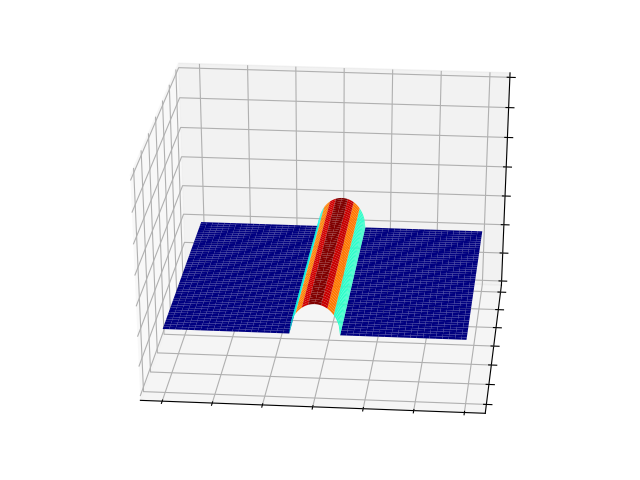
\includegraphics[width=\linewidth]{circular_trough}
      \caption{The graph of a cylindrical ridge of radius $r$,
			      	as given by $f(x,y)$ as given above.}
      \end{figure}
      
      
      We calculate the necessary partial derivatives of $f$ as follows:
      
      \begin{gather}
      \frac{\partial f}{\partial x} = \left(1, 0, \frac{-x}{\sqrt{r^2 - x^2}}\right)
      \quad , \quad
      \frac{\partial^2 f}{\partial x^2} = \left(0, 0, \frac{-r^2}{\left(\sqrt{r^2 - x^2}\right)^3}\right) \\
      \frac{\partial f}{\partial y} = \left(0, 1, 0\right)
      \quad , \quad
      \frac{\partial^2 f}{\partial y^2} = \frac{\partial^2 f}{\partial x \partial y} = 0
      \end{gather}
      The gauss map is given by
      \begin{gather}
      \nu(x,y) = \frac{\frac{\partial f}{\partial x} \times \frac{\partial f}{\partial y}}
      {\vnorm{\frac{\partial f}{\partial x} \times \frac{\partial f}{\partial y}}}
      = \left( \frac{x}{r} ,\; 0 ,\; \frac{\sqrt{r^2 - x^2}}{r} \right) \\
	  \implies
	  \frac{\partial \nu}{\partial x}
		  = \left(\frac{1}{r} \;,\; 0\;,\; \frac{-x}{r\sqrt{r^2-x^2}}\right)
		  \quad , \quad \frac{\partial \nu}{\partial y} = \left(0,0,0\right).
      \end{gather}
      
      We then calculate matrix elements of the Weingarten map's construction as given in
      \cref{hij_exactgraph} and \cref{gij_exactgraph} :
      \begin{align}
      [h_{ij}] = \frac{1}{\sqrt{1+h_x^2 + h_y^2}} \,  \Hess (h)
		       &= \frac{1}{\sqrt{1+\left(\frac{x^2}{r^2-x^2}\right)}}
		       \begin{bmatrix}
		       \frac{-r^2}{\sqrt{r^2 - x^2}^3} & 0 \\
			     0 & 0
		       \end{bmatrix} 
		       &= \begin{bmatrix}
		       \frac{-r}{r^2 - x^2} & 0 \\
		       0 & 0
		       \end{bmatrix} \\
		       [g_{ij}]^{-1} &= \begin{bmatrix} \frac{r^2 - x^2}{r^2} & 0 \\ 0 & 1 \end{bmatrix} \\
		       \implies \weinmat = [h_{ij}]	[g_{ij}]^{-1} &=
		       \begin{bmatrix}
		       \frac{-r}{r^2 - x^2} & 0 \\
		       0 & 0
		       \end{bmatrix} \begin{bmatrix} \frac{r^2 - x^2}{r^2} & 0 \\ 0 & 1 \end{bmatrix} \\
		       &= \begin{bmatrix} - \frac{1}{r} & 0 \\ 0 & 0 	\end{bmatrix}	       	
      \end{align}
      
      We see that $u_2 = (0,1)$ and $u_1 = (1,0)$ are eigenvectors for $\weinmat$ with respective eigenvalues
      $\kappa_2 = -\frac{1}{r} , \kappa_1 = 0$. Given the theorem of Olinde Rodriguez suggests that $u_2$ points in the direction of maximum curvature of the surface, $-\frac{1}{r}$, which is predictably in the direction directly perpendicular to the trough, whereas the direction of least curvature is along the trough and is $0$. The theorem of Meusnier suggests that the normal curvature $\kappa_2 = -\frac{1}{r}$ is reasonable-- any curve on the trough perpendicular to the ridge should have the curvature of a circle (the negative simply indicates that we are on the ``outside'' of the surface). Finally, we note that at the ridge of the trough is exactly where $\nabla f = 0$, and the Weingarten map is exactly the Hessian matrix there.
      
      \vcleanup{this was dropped in here. fix the transition}
      Viewing the surface in $\R^3$, we define the Hessian \vcomment{notation here, does it need to be an operator?} $\Hess$ of the surface $L$
      at a point $(x,y)$ on the surface as the matrix of its second partial derivatives:
      \begin{equation}
      \Hess(x,y) = \begin{bmatrix}
      L_{xx}(x,y) & L_{xy}(x,y) \\
      L_{yx}(x,y) & L_{yy}(x,y)
      \end{bmatrix}
      \end{equation}
      
      At any point $(x,y)$ we denote the two eigenpairs of $\Hess(x,y)$ as
      \begin{equation}
      \Hess u_i = \kappa_i u_i \; , \quad i = 1,2
      \end{equation}
      
	  \vcleanup{the eigenvectors of the Weingarten map are orthonormal. the eigenvectors of the hessian are also orthonormalizable. make the distinction!}
      where $\kappa_i$ and $u_i$ are known as the
      \textit{principal curvatures} and \textit{principal directions} \vcomment{fixthis} of $L(x,y)$, respectively, and we label such that $|\kappa_2| \ge |\kappa_1|$. Notably, $\Hess(x,y)$ is a real, symmetric matrix (since  $L_{xy} = L_{yx}$ and $L$ is a real function)and thus its eigenvalues are real and its eigenvectors are orthonormal to each other, as given by following lemma:
      
      % from burden and faires corollary 9.17
      \begin{lemma}[Principal Axis Theorem?]
      	Let $A$ be a real, symmetric matrix. The eigenvalues of $A$ are real and its eigenvectors are orthonormal to each other.
      \end{lemma}
      
      \begin{proof}
      	Let $x\ne 0$ so that $Ax = \lambda x$. Then 
      	\begin{align*}
      	\vnorm{Ax}_2^2 = \inner{Ax}{Ax}  &= (Ax)^{*} Ax \\
      	&= x^{*}A^{*}Ax = x^{*}A^T A x = x*A A x \\
      	&= x^{*} A \lambda x = \lambda x^{*} A x \\
      	&= \lambda x^{*} \lambda x = \lambda^2 x^{*} x = \lambda ^2 \vnorm{x}_2^2
      	\end{align*}
      	Upon rearrangement, we have
      	$\lambda^2 = \frac{\vnorm{Ax}_2^2}{\vnorm{x}_2^2} \ge 0 \implies \lambda $ is real.
      	
      	To prove that a set of orthonormalizable eigenvectors exists,
      	let $A$ be real, symmetric as above and consider the eigenpairs
      	$Av_1 = \lambda_1 v_1$, $Av_2 = \lambda_2 v_2$ with $v_1, v_2 \ne 0$.
      	\footnote{To simplify notation, we simplify our argument to consider two explicit eigenvectors only, since we're only concerned with the $2\times 2$ matrix $\Hess$
      		anyway.}
      	
      	In the case that $\lambda_1 \ne \lambda_2$, we have
      	\begin{align*}
      	(\lambda_1 - \lambda_2)v_1^T v_2 &= \lambda_1 v_1^T v_2 - \lambda_2 v_1^T v_2 \\
      	&= (\lambda_1 v_1)^T v_2 - v_1^T (\lambda_2 v_2) \\
      	&= (Av_1)^T v_2 - v_1^T (Av_2) \\
      	&= v_1^T A^T v_2 - v_1^T A v_2 \\
      	&= v_1^T A v_2 - v_1^T A v_2 = 0
      	\end{align*}
      	Since $\lambda_1 \ne \lambda_2$, we conclude that $v_1^T v_2 = 0$.
      	
      	In the case that $\lambda_1 = \lambda_2 =: \lambda$, we can define
      	(as in Gram-Schmidt orthogonalization) $u = v_2 - \frac{v_1^Tv_2}{v_1^Tv_1}v_1$.
      	This is an eigenvector for $\lambda=\lambda_2$, as
      	\begin{align*}
      	Au &= A\left(v_2 - \frac{v_1^Tv_2}{v_1^Tv_1} v_1\right) \\
      	&= A v_2 - \frac{v_1^Tv_2}{v_1^Tv_1} A v_1 \\
      	&= \lambda v_2- \frac{v_1^Tv_2}{v_1^Tv_1} \lambda v_1 \\
      	&= \lambda \left( v_2 - \frac{v_1^Tv_2}{v_1^Tv_1} v_1 \right) = \lambda u
      	\end{align*}
      	and is perpendicular to $v_1$, since
      	\begin{align*}
      	v_1^T u &= v_1^T\left(v_2 - \frac{v_1^Tv_2}{v_1^Tv_1}v_1\right) \\
      	&= v_1^T v_2 - \left(\frac{v_1^Tv_2}{v_1^Tv_1}\right) v_1^T v_1 \\
      	&= v_1^T v_2 - v_1^Tv_2 (1) = 0.
      	\end{align*}
      \end{proof}
      
      Thus we see that the two principal directions form an orthonormal frame at each point (x,y) within the continuous image $L(x,y)$.
      
      \vcomment{The following unverified (but intuitive) theorem is currently unnecessary but could be useful if I still want to implement the idea of tracking direction of eigenvectors along potential ridges, useful for filling in the ridge network. Like approximating the surface using derivatives.}
      The following is an \textbf{unverified claim} (which might be useful for later):
      The frame varies continuously along paths in $\R^2$
      except at points where $\Hess(x,y)$ is singular.
      To make this explicit:
      
      \begin{theorem}[Continuity of the leading principal direction]
      	Let $\theta: I:= [0,1] \to \R^2$ be a parametrized regular curve in $\R^2$ and
      	$H_\theta := \Hess_f  \circ \theta(t)$ be the matrix-valued function
      	% use the same notation as the Hessian before and cite the eqn. number from earlier
      	(where $\Hess_f$ is the $2\times 2$ Hessian of the smooth surface $f$)
      	Let $U:I \to \R^2$ be the implicitly-defined vector valued function s.t.
      	$U(t)$ is the leading eigenvector of $H_\theta$
      	(and therefore the leading principal direction of $f$). That is,
      	\begin{equation}
      	H_\theta \; U(t) = \lambda U(t) \quad \textrm{with}\quad \lambda = \rho(H_\theta)
      	\end{equation}
      	In other words, $\abs{\lambda} \ge \abs{\tilde{\lambda}}$ for any
      	$\tilde{\lambda} : H_\theta \; u = \tilde{\lambda} u$ for some $u \ne 0$.
      	
      	Then, $U(t)$ is continuous in $t$ whenever $H_f(t)$ is non-singular.
      	\vcomment{Maybe fix this so that the path avoids any nonsingular points?
      		$U(t)$ isn't even well-defined at such points anyway.}
      \end{theorem}
      \begin{proof}
      	First, we show that $U(t)$ is a well-defined function at all points $t$ where
      	$H_f(t)$ is non-singular.
      	\vtodo{FIX PROOF OR REMOVE}
      \end{proof}
      
      \vcomment{Need a transition} To we are interested in the differentiation of 2D images, we need a way
      to calculate the quantities of the previous section \vcleanup{tag}. We can simply extend these ideas of differentiation to the discrete domain.
    
\section{Calculating Derivatives of Discrete Images} 

	
	\begin{itemize}
		\item \vtodo{Describe taking gradient with divided difference.}
		\item \vtodo{Describe the situation: derivatives should be taken on Gaussian blur (equivalent to scale space development) [Lindeberg]. That is, you can take the derivative of either the convolved image, or you can take derivatives of the Gaussian itself, \textit{then} convolve.}
		\item \vtodo{Mention that derivatives can be taken in frequency space?}

%		Pseudocode for \texttt{np.gradient} which is used in calculating Hessian (code below)
%					\begin{verbatim}
%					gaussian_filtered = fftgauss(image, sigma=sigma)
%					Lx, Ly = np.gradient(gaussian_filtered)
%					Lxx, Lxy = np.gradient(Lx)
%					Lxy, Lyy = np.gradient(Ly)
%					\end{verbatim}	
		\end{itemize}
\vcomment{describe this no matter what. if you want to calculate the derivatives in frequency space,
	still describe this so you can compare the results.}
\vcleanup{Move scale space theory section before this.}


\section{The Frangi Filter} \label{sec:frangi}


    \subsection{Intro to Hessian-based filters}
	%Basic properties and observations. Why these filters make sense. Basic strengths and weaknesses.

        Hessian-based filters are a family of curvilinear filters that employ the Hessian and its eigenspaces
        to determine regions of significant curvature within an image.
        % as mentioned by Frangi, see Sato [13] and Lorenz [10] in their paper
        Several such filters exist --see Sato [13] and Lorenz[10]. These filters use information about the principal curvatures (eigenvalues of the Hessian) at each point to 
        
        
	\subsection{Implementation Details: Convolution Speedup via FFT}
	\vcomment{FIRST DESCRIBE HOW YOU NEED DERIVATIVES}
	
	As described above, the actual computation of derivatives is achieved via convolution with a gaussian. In practice, this is very slow for large scales. We instead, we perform a fast Fourier transform, which offers a speedup of $N^2$ operations vs $\mathscr{O}\left(n\cdot \log_2n\right)$ operations \vcomment{extend to 2D}

\vcleanup{Fix this part of the outline}
\section{Fourier Transforms}
	\subsubsection{Fourier Transform of a continuous 1D signal}
	
	\vcomment{start with 1D but then extend/rewrite}
	
	A periodic signal (real valued function) $f(t)$ of period $T$ can \vcomment{justify?} be expanded in an infinite basis as follows:
	
	\begin{equation}
		f(t) = \sum_{-\infty}^{\infty} c_n e^{i\frac{2\pi n}{T}t} \;,\quad
			c_n = \frac{1}{T}\int_{-T/2}^{T/2} f(t) e^{-i\frac{2\pi n}{T}t} dt
			\end{equation}
	
	The Fourier transform of a 1D continuous function is defined by
	\begin{equation} \label{1D-CFT}
		F(\mu) := \FT\{f(t)\} \;=\; \int_{-\infty}^{\infty} f(t) e^{i2\pi \mu } dt
	\end{equation}
	
	It can be shown \vcomment{justify?} that an inverse transform will then recover our original signal:
	\begin{equation} \label{1D-ICFT}
		f(t) = \FT^{-1}\left\{F(\mu)\right\} = \int_{-\infty}^{\infty} F(\mu) e^{i2\pi \mu t} dt
	\end{equation}
	
	Together, \cref{1D-CFT} and \cref{1D-ICFT} are referred to as the \textit{Fourier transform pair} of the signal $f(t)$. 
	
	\subsubsection{Fourier Transform of a Discrete 1D signal}
	
	We wish to develop the Fourier transform pair for a discrete signal. We frame the situation
	as follows: A continuous function $f(t)$ \vcomment{right now, with domain $\R$} is represented as the sampled function $\tilde{f}(t)$ by multiplying it by a sampling function (also referred to
	in DIP-GW as an impulse function), an infinite series of discrete impulses with equal spacing $\Delta T$:
	
	\begin{equation} \label{1D-sampling-function}
	s_{\Delta T}(t) = \sum_{n=-\infty}^{\infty} \delta[t - n\Delta T] \;,\quad
	\delta[t] = \begin{cases} 1 \;,\; & t=0 \\ 0 \;,\;& t \ne 0 \end{cases}
	\end{equation}
	
	where $\delta[t]$ is the discrete unit impulse.
	
	The discrete sample $f(t)$ is then constructed from $f(t)$ by
	\begin{equation} \label{1D-discrete-sample}
	\tilde{f}(t) = f(t) s_{\Delta T}(t)
	\end{equation}
	
	From this (and actually the convolution theorem) we can calculate $\tilde{F}(t)$. \vtodo{Derive this. There's some groundwork here to copy between 213-220. We don't need the sampling theorem, since our signal is given as-is... i think}.
	
	\subsubsection{1D Discrete Fourier Transform (DFT)}
	
	Given the discrete signal $\tilde{f}$, we construct the transform
	$\tilde{F}(\mu) = \FT\{\tilde{f}(t)\}$. by simply transforming the definition \cref{1D-discrete-sample}.
	
	\vcomment{supress derivation but do explain $f_n$ notation / cleanup}
	
	\begin{equation} \label{1D-DFT-transform}
	\tilde{F}(\mu) = \sum_{n=-\infty}^{\infty} f_n e^{-i 2\pi \mu n \Delta T} \;,\quad
		f_n = \tilde{f}(n) = f(n\Delta T)
	\end{equation}
	
	The transform is a continuous function with period $1 / \Delta T$. 
	
		\begin{itemize}
			\item \vtodo{find image processing papers that find hessian from FFT / who uses this?}
			\item \vtodo{with above: downsides?}
			\item \vtodo{side by side comparison in a toy example and/or a real problem?}
		\end{itemize}
		
		\subsubsection{2D Discrete Fourier Transform Convolution Theorem}\vcomment{the following was adapted in a large part from DFT: an owner's manual. cite? DIP-DW just proves the continous version (in 1D) and then asserts that it works for discrete variables too.}
		
		\vcleanup{get consistent notation--either have the discrete signals be notated as  $\tilde{f}(x,y)$ or $f[x,y]$ or instead comment that it's understood}
		\begin{theorem}[2D DFT Convolution Theorem] 
			\vcomment{develop the 2-D DFT from Sec. 4.3 4.4 from DIP-GW (see p235).}
		Given two discrete functions are sequences with the same length \vtodo{don't gloss over this} \vcomment{If they're not actually the same length, DIP-GW suggests to make the final length at least $P = A+C-1$ and $Q = B+D-1$ in the case that the sizes are $A\times B$ and $C\times D$ for $f(x,y)$ and  $h(x,y)$ respectively. Not sure if that matters.}, that is:
		$f(x,y)$ and $h(x,y)$ for integers $0 < x < M$ and $0 < y < N$, we can take the discrete fourier transform (DFT) of each:
		\begin{align}
		F(u,v) := \mathcal{D}\{f(x,y)\} &=
						\sum_{x=0}^{M-1} \sum_{y=0}^{N-1} f(x,y)
						e^{-2\pi i \left(\frac{ux}{M} + \frac{vy}{N}\right)} \\	
		   H(u,v) := \mathcal{D}\{h(x,y)\} &=
						\sum_{x=0}^{M-1} \sum_{y=0}^{N-1} h(x,y)
						e^{-2\pi i \left(\frac{ux}{M} + \frac{vy}{N}\right)}
		\end{align}
		
		and given the convolution of the two functions
		\begin{equation}
		\left(f \star h\right)(x,y) = \sum_{m=0}^{M-1} \sum_{n=0}^{N-1} f(m,n)h(x-m,y-n)
		\end{equation}
		
		then $\left(f \star h\right)(x,y)$ and $MN\cdot F(u,v)H(u,v)$ are transform pairs, i.e.
		\begin{equation}
		\left(f \star h\right)(x,y) = \mathcal{D}^{-1}\left\{MN\cdot F(u,v)H(u,v)\right\}
		\end{equation}
		\end{theorem}
		
		
		The proof follows from the definition of convolution, substituting in the inverse-DFT of $f$ and $h$, and then rearrangement of finite sums.
		\begin{proof}
		\begin{align}
		\left(f \star h\right)(x,y) &= \sum_{m=0}^{M-1} \sum_{n=0}^{N-1} f(m,n)h(x-m,y-n) \\
		&= \sum_{m=0}^{M-1} \sum_{n=0}^{N-1}
		\left(\sum_{p=0}^{M-1} \sum_{q=0}^{N-1} F(p,q)
			e^{2\pi i \left(\frac{mp}{M} + \frac{nq}{N}\right)}\right)
			\left(\sum_{u=0}^{M-1} \sum_{v=0}^{N-1} H(u,v)
			e^{2\pi i \left(\frac{u(x-m)}{M} + \frac{v(y-n)}{N}\right)} \right) \\
		&= \left(\sum_{u=0}^{M-1} \sum_{v=0}^{N-1} H(u,v)
			e^{2\pi i \left(\frac{ux}{M} + \frac{vy}{N}\right)}\right)
			\left(\sum_{p=0}^{M-1} \sum_{q=0}^{N-1} F(p,q)
			\left(\sum_{m=0}^{M-1} e^{2\pi i \left(\frac{m(p-u)}{M}\right)}\right)
			\left(\sum_{n=0}^{N-1} e^{2\pi i \left(\frac{n(q-v)}{N}\right)}\right)\right) \\
			&= \left(\sum_{u=0}^{M-1} \sum_{v=0}^{N-1} H(u,v)
			e^{2\pi i \left(\frac{ux}{M} + \frac{vy}{N}\right)}\right)
			\left(\sum_{p=0}^{M-1} \sum_{q=0}^{N-1} F(p,q)
			\left( M \cdot \hat{\delta}_M(p-u) \right)
			\left( N \cdot \hat{\delta}_M(q-v)\right)\right) \\
			&= \left(\sum_{u=0}^{M-1} \sum_{v=0}^{N-1} H(u,v)
			e^{2\pi i \left(\frac{ux}{M} + \frac{vy}{N}\right)}\right)
			\cdot M N F(u,v) \\
			&=MN \cdot \sum_{u=0}^{M-1} \sum_{v=0}^{N-1} F(u,v) H(u,v)
			e^{2\pi i \left(\frac{ux}{M} + \frac{vy}{N}\right)} \\
			&= MN \cdot \mathcal{D}^{-1}\left\{ FH\right\}
		\end{align}
		
		where
		\begin{equation} \label{delta_multiple}
			\hat{\delta}_N (k) = \begin{cases}
				1 & \text{when } k = 0 \mod N \\
				0 & \text{else}
				\end{cases}
		\end{equation}
	\end{proof}
	Above, we make use of the following lemma \vcomment{add this before DFT convolution theorem and embed the definition of $\hat{\delta}_N$ inside}
	\begin{lemma}
	Let $j$ and $k$ be integers and let $N$ be a positive integer. Then
	\begin{equation} \label{dft_conv_lemma}
		\sum_{n=0}^{N-1} e^{2\pi i\left(\frac{n(j-k)}{N}\right)} =  N \cdot \hat{\delta}_N(j-k) 
		\end{equation}
		\end{lemma}
		\begin{proof}
		
		Consider the complex number $e^{2\pi i (j-k)/N}$. Note first that this is an $N$-th root of unity, since
		\[
		\left(e^{2\pi i (j-k)/N}\right)^N = e^{2\pi i (j-k)} = \left(e^{2\pi i}\right)^{(j-k)}
		= 1^{(j-k)} = 1
		\]
	
	In other words, $e^{2\pi i n(j-k)/N}$ is a root of $z^N -1 = 0$, which we can factor as
	\begin{equation}
	z^N -1 \;=\; (z-1)\left(z^{n-1} + \cdots + z + 1\right) \;=\; (z-1)\sum_{n=0}^{N-1} z^n .
	\end{equation}

thus giving us
\begin{equation} \label{dft_conv_lemma_factors}
	0 = \left(e^{2\pi i(j-k)/N} - 1\right) \sum_{n=0}^{N-1} e^{2\pi i n(j-k)/N}
	\end{equation}
	
To prove the claim in \cref{dft_conv_lemma}, we consider two cases: First, if $j-k$ is a multiple of $N$, we of course have $e^{2\pi i n(j-k)/N} = \left(e^{2\pi i}\right)^{n(j-k)/N} = 1$  and thus the left side of \cref{dft_conv_lemma} reduces to 
\[
\sum_{n=0}^{N-1} \left(e^{2\pi i}\right)^{n(j-k)/N} = \sum_{n=0}^{N-1} \left(1\right) = N
\].

In the case that $j-k$ is \textit{not} a multiple of $N$, we refer to \cref{dft_conv_lemma_factors}.
The first factor is not zero since, $\left(e^{2\pi i (j-k)/N}\right) \ne 1$ (simply since $(j-k)/N$ is not an integer), and thus it must be that the second factor is 0:
\[
\sum_{n=0}^{N-1} \left(e^{2\pi i (j-k)/N}\right)^n = 0\]
	
	We can combine these two cases by invoking the definition of \cref{delta_multiple}, giving us the result.
		\end{proof}
				
		\subsubsection{FFT}
		 \vcomment{use DIP-GW p298}
		As noted, the above result applies to the Discrete Fourier Transform. As noted, we actually achieve a convolution speedup using a Fast Fourier Transform (FFT) instead. We follow the developments of DIP-GW \vcomment{should I? or just link? or fix notation? or do for 2D at the same time}. For clarity, we present the following theorems which allow a framework to calculate a 2D Fourier transforms quickly.
		
		
		First, a 2D DFT may actually be calculated via two successive 1D DFTs, which can be
		seen through a basic rearrangement, as follows:
		
		\begin{align}
		F(\mu,\nu) &= \sum_{x=0}^{M-1} \sum_{y=0}^{N-1} f(x,y) e^{-i2\pi \left(\mu x/M + \nu y/N\right)} \\
			   &= \sum_{x=0}^{M-1} e^{-i2\pi \mu x/M} \left[ \sum_{y=0}^{N-1} f(x,y)e^{-i2\pi \nu y/N} \right] \\
			   &= \sum_{x=0}^{M-1} e^{-i2\pi \mu x/M} \FT_x\{ f(x,y)\} \\
			   &= \FT_y\{\FT_x \{f(x,y)\} \}
		\end{align}
		
		where $\FT_{x'}$ refers to the 1D discrete Fourier transform of the function with respect to
		the variable $x'$ only.
		
		Thus, to calculate the fourier transform $F(u,v)$ at the point $u,v$
		requires the computation of the transform of length $N$ for each iterated point $x \in 0..M-1$. Thus there are $MN$ complex multiplications and $(M-1)(N-1)$ complex additions in this sequence required for each point $u,v$ that needs to be calculated. Overall, for all points that need to be calculated, the total order of calculations is on the order of $(MN)^2$ \vcomment{rectify this, is it really caused by the number of $u,v$ points that need calculating?}. (Note: the values of $e^{-i2\pi m/n}$ can be provided by a lookup table rather than ad-hoc calculation \vcomment{source?}.
		
		We now show that a considerable speedup can be achieved through elimination of redundant calculations. In particular, we wish to show that the calculation of a 1D DFT of signal length $M=2^n, n \in \Zpos$ can be reduced to calculating two half-length transforms and an additional $M/2 = 2^{n-1}$ calculations.
		
		\vcomment{we follow DIP-GW variable conventions, which I think are dumb}
		
		To "simplify" our notation we will use a new notation for the Fourier kernels/basis functions.
		Let the 1D Fourier transform be given by
		
		\begin{equation} \label{FFT-defineW}
		F(u) = \sum_{x=0}^{M-1} f(x) W_M^{ux},\quad \textrm{where} \quad W_m := e^{-i2\pi/m}
		\end{equation} 
		
		We'll define $K \in \Zpos : 2K = M = 2^n$ (i.e. $K = 2^{n-1})$.
		
		We use this to rewrite the series in \cref{FFT-defineW} and split it into odd and even entries in the summation
		
		\begin{align}
		F(u) &= \sum_{x=0}^{2K-1} f(x) W_{2K}^{ux} \\
			 &= \sum_{x=0}^{K-1} f(2x) W_{2K}^{u(2x)}
				 + \sum_{x=0}^{K-1} f(2x+1) W_{2K}^{u(2x+1)} \label{FFT-oddevensplit}
		\end{align}
		
		We'll get a few identities out of the way (where $m, n, x \in \Zpos$ arbitrary).
		
		\vcomment{this fixes an issue in DIP-GW where the identities were provided in terms of $M$ instead of arbitrary $m$, where the proof uses the results for some value other than $M$ anyway}
		\begin{gather} \label{fft-kernelidentities}
		W_{(2m)}^{(2n)} = e^{\frac{-i2\pi(2m)}{2m}} = e^{\frac{-i2\pi m}{n}} = W_{m}^{n} \\
		W_{m}^{(u+m)x} = e^{\frac{-i2\pi(u+m)x}{m} } = e^{\frac{-i2\pi unx}{m}} e^{\frac{-i2\pi mx}{m}}
					= e^{\frac{-i2\pi ux }{m}} (1) = W_m^{ux} \\
		W_{2m}^{(u+m)} = e^{\frac{-i2\pi(u+m)}{2m}} = e^{\frac{-i2\pi ux}{2m}} e^{-i\pi}
					 = W_{2m}^{u} e^{-i\pi} = - W_{2m}^{u}
		\end{gather}

Thus we can rewrite \cref{FFT-oddevensplit} as
\begin{align}
F(u)  &= \sum_{x=0}^{K-1} f(2x) W_{2K}^{2ux} + \sum_{x=0}^{K-1} f(2x+1) W_{2K}^{2ux} W_{2K}^{u} \\
\Longrightarrow \quad F(u) &= \left(\sum_{x=0}^{K-1} f(2x) W_{K}^{ux}\right)
	 + \left(\sum_{x=0}^{K-1} f(2x+1) W_{K}^{ux}\right) W_{2K}^{u}
		 \label{fft-oddeven-parens}
\end{align} 

The major advance comes via using the identities \cref{fft-kernelidentities} \vcleanup{fix multitag} to consider the Fourier transform $K$ 
frequencies later \vcomment{wording?}:
\begin{align}
F(u+K) &= \left(\sum_{x=0}^{K-1} f(2x) W_{K}^{(u+K)x}\right)
+ \left(\sum_{x=0}^{K-1} f(2x+1) W_{K}^{(u+K)x}\right) W_{2K}^{(u+K)}\\
\Longrightarrow F(u+K) &= \left(\sum_{x=0}^{K-1} f(2x) W_{K}^{ux}\right)-\left(\sum_{x=0}^{K-1} f(2x+1)W_K^{ux}\right) W_K^{u}
\label{fft-oddeven-parens-plusK}
\end{align}


Comparing \cref{fft-oddeven-parens} and \cref{fft-oddeven-parens-plusK}, we see that the expressions within parentheses are identical.
	What's more, these parentetical expressions are functionally identical to discrete fourier transforms themselves! Let's notate them as follows:
	\begin{align} \label{fft-oddeven-subdfts}
	\DFT_u\{f_{\mathrm{even}}(t)\} &:= \sum_{x=0}^{K-1} f(2x)W_K^{ux} \\
	\DFT_u\{f_{\mathrm{odd}}(t)\} &:= \sum_{x=0}^{K-1} f(2x+1)W_K^{ux}
	\end{align}
	
	If we're calculating an $M$ point transform \vtodo{vocabulary also how many frequencies do we calculate? same as \# samples? what do we need?} (i.e. we're wishing to
	calculate $F(1), ... , F(M))$, once we've calculated the first $K$ discrete frequencies (i.e. $F(1), .. , F(K))$ we may simply reuse the two values we've calculated in \cref{fft-oddeven-subdfts} to calculate the next $F(K+1),..,F(K+K) = F(M)$. Since each expression in parentheses involves $K$ complex multiplications and $K-1$ complex additions, we are effectively saving $K(2K-1)$ calculations in computing the entire spectrum  $F(1), ..,  F(M)$. When $M$ is large, the payoff is undeniable.

In fact, through counting calculations and then doing a proof by induction, we can show that the effective number of calculations is given by $M\log_2{M}$. \vtodo{finish this}.

Of course, since \cref{fft-oddeven-subdfts} are DFTs themselves, there's nothing stopping us from reiterating this procedure; if $M$ is substantially large, we can just as easily repeat this process a few times.

Of course, our development was for $1D$.  We can extend this to $2D$ by taking note of \vcleanup{cite previous section or move section here.}
	
The one caveat is that the above development was for transforming sequences whose lengths are perfect powers of $2$. Since our inputs have no reason to be this, we need to adjust for this. The explanation is \vtodo{probably} that you just do the part that's a power of 2 and  then do the rest manually or pick a different power. See \vtodo{find out how fft-pack does this}


The inverse DFT is actually a DFT of a modified function, see \vtodo{cite DIP-GW here or show that}. \vtodo{check how fftpack does this}

\hrulefill
\section{Linear Scale Space Theory}
	\vcomment{this is all as cited in GSST book (see starting in sec 6.3.1).
		as mentioned there, this is analogous to a discrete development
		(lindeberg 1990 lindeberg 1991 lindeberg 1994c lindeberg 1994e)}
	
	Koenderink showed/asserted that "any image can be embedded in a one-parameter family of derived images (with resolution as the parameter) in essentially only one unique way" given a few of the so-called \textit{scale space axioms}. They showed in particular that any such family must satisfy the heat equation
	\begin{equation}
		\Delta K(x,y,\sigma) = K_\sigma (x,y,\sigma) 
		\;\text{for}\; \sigma \ge 0
		\;\text{such that}\; K(x,y, 0) = u_0(x,y).
		\end{equation}
		
		where $K: \R^3 \to \R $ and  $u_0: \R^2 \to \R: $ is the original image (viewed as a continuous surface) and $\sigma$ is a resolution parameter.
	Much work has been done to formalize this approach. There is a long list of desired properties
	quoted from gsst. goal is to try to find a minimal subset of axioms and show that other desired properties follow.
	
	
\subsection{Axioms}
	To make matters manageable, [PEOPLE] have taken the approach of requiring the one-parameter family of scaled images to be generated by an operation.
	
	\subsection{Linear-shift invariance}
		This requires that the generator is convolution by some kernel. Show or proclaim.
		Shift-invariant means that no position in the original signal is favored (makes sense, this should apply to any image.)
	
	\subsubsection{Rotational invariance}
		Similar to above, no favoritism to directionality.
	
	\subsubsection{Semigroup property}
		They stack (no preferred scale)
	
	\subsubsection{Causality condition}
		No ``spurious resolution'' can be generated as parameter increases. \vcomment{FIX NOTATION}
		If $K(x_0,y_0;z_0)$ is a local maximum (in space)
			(i.e. $\nabla_{x,y}K(x_0,y_0; z_0) = 0 \;,\; \Delta_{x,y} K(x_0,y_0;z_0) < 0$ ),
			then an increase in scale can only weaken this peak, i.e.
			\begin{equation}
			z_0 > z_1 \implies K(x_0,y_0;z_0) \ge K(x_0,y_0;z_1)
			\end{equation}
		Similarly, if $K(x_0,y_0;z_0)$ is a local minimum (in space), (i.e. $\nabla_{x,y}K(x_0,y_0; z_0) = 0 \;,\; \Delta_{x,y} K(x_0,y_0;z_0) > 0$ ),
		then an increase in scale cannot make such a valley more profound, i.e.
		\begin{equation}
		z_0 > z_1 \implies K(x_0,y_0;z_0) \le K(x_0,y_0;z_1)
		\end{equation}
	
	This implies that no image feature is sharpened by an decrease and resolution--the only result is a flattening out of the image as scale parameter $z$ tends to infinity.s
	
	
	\subsubsection{Linearity of generator}
	``Linearity implies that all-scale space properties valid for the original signal will transfer to its derivatives. Hence, there is no commitment to certain aspects of image structure, such as the zero-order representation, or its first- or second-order derivatives.''
	\vcomment{this is dubious, as mentioned by JvB}


\subsection{Necessity of convolution}
	Where is this.
\subsection{Uniqueness of the Gaussian Kernel}
	Proved \vcomment{however artificially} by Koenderink [1984] and Babaud [1986] that such an axiomatic foundation requires that the family is generated by convolution with a kernel. The remainder of the development is to the determine that the kernel is exactly the Gaussian.
	 
	 \vtodo{TODO:
		JUST EVEN OUT THE ABOVE.
		FIND SOMETHING TO JUSTIFY CONVOLUTION.
		CITATIONS FOR LATER FORMULATIONS.
		BUILD UP HEAT EQUATION (HOWEVER RIGOROUSLY YOU CAN).
		SHOW NECESSITY OF GAUSSIAN (OR DON'T).
	}
		

	 To this, show that:
		 \begin{itemize}
		 	\item a kernel satisfying the above axioms must satisfy the heat equation
		 	\item the gaussian kernel satisfies that.
		 	\item gaussian kernel is the only kernel that works (koenderink paper?)
		 \end{itemize}


\subsection{$G_\sigma \star u_0$ solves the heat equation}
	given $u_0$ as a continuous image (unscaled), we construct PDE with this as a boundary condition.
	
	\begin{equation}
		u: \R^2 \supset \Omega \to \R \; \textrm{with} \; u(\bm{x},t) : \;
			\begin{cases}
				\frac{\partial u}{\partial t} (\bm{x}, t) = \Delta u(\bm{x},t) & ,\; t \ge 0 \\
				u(\bm{x},0) = u_0(\bm{x}) 
			\end{cases}
		\end{equation}

	We show that
	\begin{equation}
		u(\bm{x},t) = \left(G_{\sqrt{2t}} \star u_0 \right)(\bm{x})
	\end{equation}
	solves (the above tagged equation), where
	\[
		G_\sigma := \frac{1}{2\pi \sigma^2} e^{\left(-\abs{x}^2 / (2\sigma^2)\right)}
	\]
	First, we need a quick lemma regarding differentiation a continuous convolution.
	\begin{lemma} \label{dconvolution}
		Derivative of a convolution is the way that it is (obviously rewrite this).
	\end{lemma}
	\begin{proof}
		For a single variable,
		\begin{align}
		\frac{\partial}{\partial \alpha} \left[ f(\alpha) \star g(\alpha) \right]
		&= \frac{\partial}{\partial \alpha} \left[ 
		\int f(t) g(\alpha - t) dt \right] \\
		&=  \int f(t) \frac{\partial}{\partial \alpha}\left[ g(\alpha - t)  \right] dt \\
		&=  \int f(t) \left(\frac{\partial g}{\partial \alpha}\right) g(\alpha - t) dt \\
		&=  f(\alpha) \star g'(\alpha)
		\end{align}
		By symmetry of convolution we can also conclude 
		\[\frac{\partial}{\partial \alpha} \left[ f(\alpha) \star g(\alpha) \right]
		= f'(\alpha) \star g(\alpha)
		\]
		
		If $f$ and $g$ are twice differentiable, we can compound this result to show a similar statement holds for second derivatives, and then, given the additivity of convolution,
		we may conclude
		\begin{equation}
		\Delta \left(f \star g \right) = \Delta(f) \star g = f \star \Delta(g) 
		\end{equation} 
	\end{proof}
	\begin{theorem}
		$u(\bm{x},t) = \left(G_{\sqrt{2t}} \star u_0 \right)(\bm{x})$ solves the heat equation.
	\end{theorem}
	\begin{proof}
		We focus on the particular kernel
		\[
			G_{\sqrt{2t}} = \frac{1}{4\pi t} e^{\left(-\abs{x}^2 / (4t)\right)}
			\]
	
	
	Then
	\begin{align}
	\frac{\partial u}{\partial t} (\bm{x}, t)
		&= \frac{\partial}{\partial t} \left(G_{\sqrt{2t}}(\bm{x},t) \star u_0(\bm{x})\right)  \\
		&= \frac{\partial}{\partial t} \left(G_{\sqrt{2t}}(\bm{x},t)\right) \star u_0(\bm{x})  \\
		&= \frac{\partial}{\partial t} \left(
			\frac{1}{4\pi t} e^{\left(-\abs{x}^2 / (4t)\right)} \right) \star u_0(\bm{x}) \\
		&= \left[
		-\frac{1}{4\pi t^2} e^{\left(-\abs{x}^2 / (4t)\right)}
			+ \frac{1}{4\pi t}\left(\frac{-\abs{x}^2}{4t^2}\right) e^{-\abs{x}^2 / (4t)}
			\right] \star u_0(\bm{x}) \\
			&= -\frac{1}{4t^2} \left( e^{\left(-\abs{x}^2 / (4t)\right)} 
					+ \abs{\bm{x}}^2 G_{\sqrt{2t}}(\bm{x},t)
						\right) \star u_0(\bm{x})
	\end{align}
	and from the previous lemma,
	\[
	\Delta u(\bm{x}, t) = \Delta\left( G_{\sqrt{2t}} \star u_0(\bm{x})\right)
						= \Delta\left( G_{\sqrt{2t}} \right)\star u_0(\bm{x})
	\]
	
	We explicitly calculate the Laplacian of $G_{\sigma}(x,y) = A \exp(-\frac{x^2 + y^2}{2\sigma^2})$ as follows:
	
	\begin{align*}
	\frac{\partial}{\partial x} G_{\sigma}(x,y)
		&= A \left( \frac{-2x}{2\sigma^2}\right) \exp\left(-\frac{x^2 + y^2}{2\sigma^2}\right) \\
		\implies \frac{\partial^2}{\partial^2 x} G_{\sigma}(x,y)
		&= A \cdot \frac{\partial}{\partial x}
		\left[ - \frac{x}{\sigma^2} \exp\left(-\frac{x^2 + y^2}{2\sigma^2}\right) \right] \\
		&= A \left[ - \frac{1}{\sigma^2} \exp\left(-\frac{x^2 + y^2}{2\sigma^2}\right) 
			+ \frac{x}{\sigma^2} \cdot \frac{2x}{2\sigma^2} \exp\left(-\frac{x^2 + y^2}{2\sigma^2}\right) \right] \\
			&= A \exp\left(-\frac{x^2 + y^2}{2\sigma^2}\right)
				\left[ - \frac{1}{\sigma^2} + \frac{x^2}{\sigma^4} \right] \\
				&= \frac{1}{\sigma^2} G_\sigma(x,y)  \left[ \frac{x^2}{\sigma^2} - 1\right]
	\end{align*}
	
	By symmetry of argument we also may conclude
	\[
	\frac{\partial^2}{\partial y^2} G_{\sigma}(x,y) = \frac{1}{\sigma^2} G_\sigma(x,y)  \left[ \frac{y^2}{\sigma^2} - 1\right]
	\]
	
	and so
	
	\begin{equation}
	\Delta G_\sigma(x,y) =
		\frac{\partial^2}{\partial x^2} \left(G_{\sigma}\right)
		+ \frac{\partial^2}{\partial y^2} \left(G_{\sigma}\right)
		= \frac{1}{\sigma^2} G_\sigma(x,y) \left[ \frac{x^2 + y^2}{\sigma^2} - 2\right] 
	\end{equation}
	Then, given \cref{dconvolution}, we conclude
	\begin{equation}
	\Delta \left[ G_\sigma(x,y) \star u_0(x,y) \right] 
	= \left(\frac{1}{\sigma^2} G_\sigma(x,y) \left[ \frac{x^2 + y^2}{\sigma^2} - 2\right]\right) \star u_0(x,y)
	\end{equation}
	
	For particular choices of $\sigma(t) = \sqrt{2t}$ and $A = \frac{1}{4\pi t}$,
	we see 
	\begin{align}
		\Delta \left[ G_{\sqrt{2t}}(x,y) \star u_0(x,y) \right] 
		&= \left(\frac{1}{2t} G_{\sqrt{2t}}(x,y) \left[ \frac{x^2 + y^2}{2t} - 2\right]\right) \star u_0(x,y) \\
		&= \left(G_{\sqrt{2t}}(x,y) \left[ \frac{x^2 + y^2}{4t^2} - \frac{1}{t}\right]\right) \star u_0(x,y)
	\end{align}
	We then calculate the time derivative,
	using our particular choice of $\sigma(t) = \sqrt{2t}$ and $A = \frac{1}{4\pi t}$ as:
	
	\begin{align}
	\frac{\partial}{\partial t} \left[ G_{\sigma(t)}(x,y) \star u_0(x,y) \right]
	&= \frac{\partial}{\partial t} \left[ G_{\sigma(t)}(x,y) \right] \star u_0(x,y) \\
	&= \frac{\partial}{\partial t} \left[ G_{\sqrt{2t}}(x,y)\right] \star u_0(x,y) \\
	&= \frac{\partial}{\partial t} \left[
	\frac{1}{4\pi t} \exp\left(-\frac{x^2 + y^2}{4t}\right) \right] \star u_0(x,y) \\
	&= \left[ -\frac{1}{4\pi t^2} \exp\left(-\frac{x^2 + y^2}{4t}\right) + 
	\frac{1}{4\pi t}\left( \frac{x^2 + y^2}{4t^2} \exp\left(-\frac{x^2 + y^2}{4t}\right)\right)
		\right] \star u_0(x,y) \\
		&= \left(G_{\sqrt{2t}}(x,y) \left[ \frac{x^2 + y^2}{4t^2} -\frac{1}{t}\right]\right) \star u_0(x,y)
	\end{align}

	Combining these results, we find that
	\begin{equation}
	\frac{\partial}{\partial t} \left[ G_{\sqrt{2t}} \star u_0 \right]
	= \Delta \left[ G_{\sqrt{2t}} \star u_0 \right] 
	\end{equation}
	
	as desired. \end{proof}
\hrulefill
\subsection{Alternative formulations of Scale Space Theory}
	Mention discrete treatments, mention relaxation of some of the dubious axioms.
\section{Morphology}
	Methods of merging multiscale methods.
	
	
\hrulefill

\section{Overview of Frangi vesselness measure}

\vcleanup{move to next section? or cover any necessary math here}

The Frangi filter \cite{frangi1998multiscale} is a widely used \vcomment{citation needed} Hessian-based filter used to detect curvilinear structures in images.  It was orignally developed for images such as MRIs and it excels in that context. It essentially relies on measuring eigenvalues of the Hessian $\Hess_\sigma(x,y)$ at some particular scale $\sigma$ at each point $(x,y)$ in the image and comparing their magnitudes.

The procedure for a single scale in a 2D image is as follows:

\vcleanup{redefine this in a sensible way so you can easily talk about the point in the domain of the image, etc.}
Let $\lambda_1, \lambda_2$ be the two eigenvalues of the Hessian of the image at point $(x_0, y_0)$,
ordered such that $\abs{\lambda_1} \leq \abs{\lambda_2}$, and define the Frangi vesselness measure at scale $\sigma$ as:


\begin{equation} \label{eq:frangi-vesselness-measure}
V_\sigma(x_0,y_0) = \begin{cases}
0 & \text{if} \quad \lambda_2 > 0 \\
\exp\left(-\frac{A^2}{2\beta^2}\right)
\left(1 - \exp(-\frac{S^2}{2c^2})\right) & \text{else}
\end{cases} \end{equation}
where
\begin{equation} \label{frangi-def-anisotropy-structureness}
A := \abs{\lambda_1 / \lambda_2}
\quad \textrm{and} \quad 
S := \sqrt{\lambda_1^2 + \lambda_2^2}
\end{equation}
and $\beta$ and $c$ are tuning parameters. Before we discuss appropriate values for $\beta$ and $c$, we first seek to highlight the significance of \cref{frangi-vesselness-measure}, and in particular, the ratios defined in
\cref{frangi-def-anisotropy-structureness}. $A$ and $S$ are known as the anisotropy measure and structureness measure, respectively. \vcleanup{define these earlier than the vesselness measure so that the definitions are easier to find}.

\subsection{Anisotropy} \label{sec:frangi.anisotropy}
The anisotropy (or directionality) measure $A$ is simply the ratio of magnitudes of $\lambda_1$ and $\lambda_2$. Since at a ridge point of a tubular structure, we should have $\lambda_1 \approx 0$ and $\abs{\lambda_2} \gg \abs{\lambda_1}$,
a very small value of $A$ would be present at a ridge of a tubular structure.

\begin{figure}[h] \label{fig:expo-principal-curvatures}
	\begin{center}
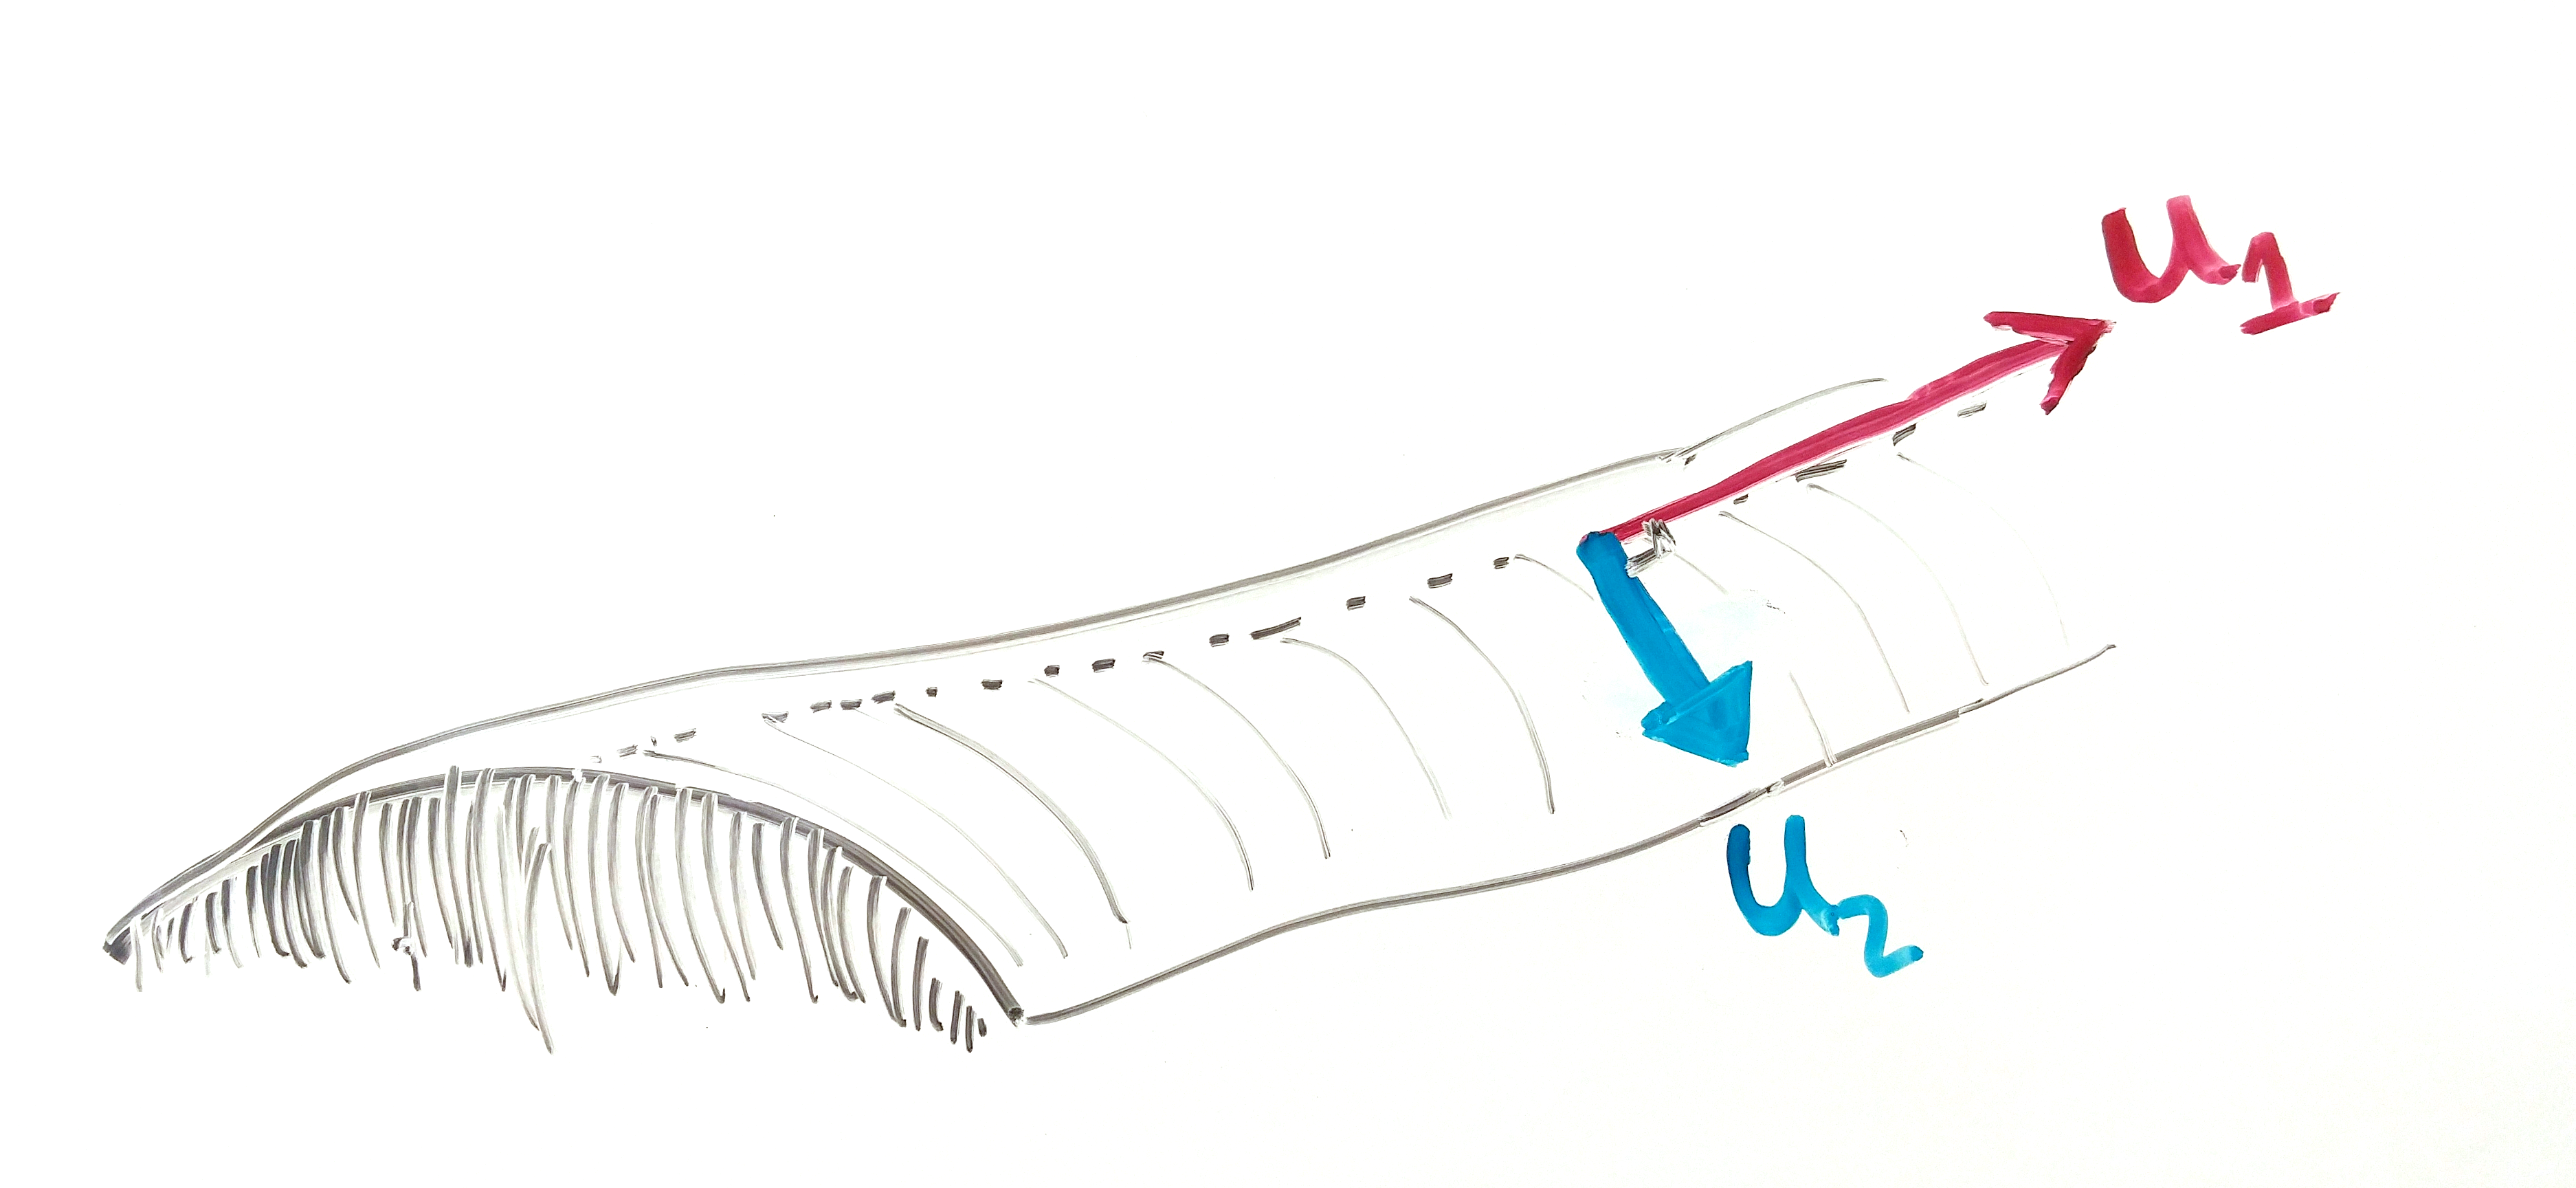
\includegraphics[width=0.8\linewidth]{expo_principal_curvatures}
\caption{The principal eigenvectors of the image $L$ at a ridge like structure (arrows not to scale). $\lambda_1 \approx 0$ and $\lambda_2$ is large and negative. \vtodo{fix drawing so $u_1$ is more to scale }}
\end{center}
\end{figure}

In \cref{fig:expo-principal-curvatures}, this situation is demonstrated. Here, $u_1, u_2$ is the orthogonal set of Hessian eigenvectors with corresponding eigenvalues $\lambda_1$ and $\lambda_2$. At such a ridgelike structure, we could predict the largest change in curvature to be straight down the ridge (in the direction of $u_2$), and the direction of least curvature to be directly along the ridge (in the direction  of $u_1$).

Of course, if the the ridge is perfectly circular along its cross section (as was in \cref{sec:calculate-weinmap-of-a-ridge}, it is of course apparent that $\lambda_2$ would be the same value at any place along the ridge (not just at its crest \vcleanup{fix terminology}), and $\lambda_1$ would likewise be 0 at any such point. Thus, the anisotropy measure will not necessarily be a maximum at the crest of the ridge. One could also imagine a similar situation in which the dropoff from crest to bottom gets increasing steep. In such a case, $\lambda_2$ as a function of $x$ would in fact be largest nearest to the bottom. This thought experiment should dispel a naive misunderstanding of the power of a frangi filter: a high anisotropy measure (and a large structureness measure \vcleanup{define structureness first}) will not in general identify the crests of a ridgelike structure--it only will highlight that such a pixel is on a ridgelike structure at all.

Similiarly, the vessel we're trying to identify can not be reasonably expected to behave as perfectly as our toy example. There will likely be small aberrations in a ridgelike structure we seek to identify.  (either small parts where it goes up (so that $u_1$ is not exactly zero \vtodo{and we could fix this by checking that it's continuousish?}, there may be small divots where the thing seems to go up a bit etc etc etc or sampling error cos it's a fucking picture etcetc \vtodo{flesh this out}.

\vcleanup{move elsewhere} Importantly, this formulation does allow that $\lambda_1$ is not necessarily approximately $0$, just that the curvature in the downward direction is much more significant.

Also the crest could be really flat, in which case both are around zero. again, this is a scaling issue.

The fix to this is to look at scale and make sure we're dealing with an appropriate scale. Also the fix is to find the ridge using a separate technique.

Also look at where the stitches are (discontinuities in $u_2,$ but $u_1$ still 0?)

\subsection{Structureness measure} \label{sec:frangi-structureness}

There is another concern with using the pure ratio $S:= \abs{\lambda_1 / \lambda_2}$ as an identifying feature of ridgelike structures: we could still have $\abs{\lambda_2} \gg \abs{\lambda_1}$ in a relative sense, but still have $\lambda_2 \approx 0$. As a rather extreme example, we should certainly wish to differentiate a point on the surface where $\lambda_2 \approx 10^{-5} $ and $\lambda_1 \approx 10^{-10}$ from another point where $\lambda_2 \approx 10000$ and $\lambda_2 = 0.1$. A quite simple fix to differentiate these points is to introduce a ``structureness'' measure to insure that there is in fact some significant curvilinear activity at the point in question. Frangi used $S:= \sqrt{(\lambda_1)^2 + (\lambda_2)^2}$, which is in fact the 2-norm of the Hessian matrix \vcleanup{show?}.

\vcleanup{note somewhere (maybe in a section called 'tuning parameters' how important this one is}


\subsection{The Frangi vesselness filter: Basic Anatomy}

Our goal then is to attach a numerical measure to each pixel in the image (at a particular scale $\sigma$) that is large when the anisotropy measure $A$ and the structureness measure $S$ is sufficiently large.

The form Frangi arrived at in \cref{eq:frangi-vesselness-measure} in which a factor of $\exp\{...\}$ and $(1 - \exp\{\})$ are multiplied together are simply to ensure that the final vesselness measure $V$ is largest when $A$ is small and $S$ is large enough, with rapidly decay in other situations.

We have an added case present in \cref{eq:frangi-vesselness-measure}, simply to ensure that $\lambda_2$ is not positive. If we are indeed at a curvilinear ridge, we need the second derivative of the surface in the maximal direction to be negative, which hasn't been accounted for as yet in our formulation of $A$ and $S$ -- we wish (for our purposes) to only indentify when we are finding crests. $A$ will still be small and $S$ will still be large however if we identify a ``trough''.
The only perceivable difference is that the maximum normal curvature will be positive--we are at a local minimum in the direction of $u_2$. In situations where we wish to only identify ridges (as is the case here) we simply exclude any points where there is not a negative curvature in the maximal direction. 

\vtodo{can you plot this theoretically to show when $V$ is large? Good parameters? Like show multiple peaks of $\exp(\dots)$ and  $(1 - \exp(\dots))$ arranged so that they only coincide in 'good' regions and are rapidly diminishing overlap elsewhere?}

\subsection{The Frangi vesselness filter: Choosing parameters $\beta$ and $c$}

The parameters $\beta$ and $c$ are meant to scale so that the peaks of $exp$ and $1-exp$ coincide enough to be statistically significant but rapidly decay in areas not associated with curvilinear structure.

What values of these parameters are appropriate is ultimately dependent on the context of the problem.

Frangi suggested for $c$ that half of the Frobenius norm of the Hessian matrix is appropriate , simply because the minimum value of $S$ is zero, and  its maximum value is approx the 2 norm of the Hessian. \vtodo{find your proof/add proof}. For $\beta$ we would say that a good intermediate point is 0.5.
(thus $2\beta^2 = 1/2$). \vtodo{analyze/show an example of what this does in the context of particular values of $\lambda_1,\lambda_2$ in terms of $V$ output}.

As we will show later, choosing $c$ freely is rather important for the context especially if the background (non-ridgelike structure) is significant and noisy. $\beta$ should be strengthened/relaxed depending on how ``flat'' the ridgelike structure is. If there is a lot of gain \vtodo{explain better or make a picture.} then $\beta$ should be smaller. If this is not the case, a stronger filter can be created by requiring $A$ to be much smaller.

\subsection{A multiscale approach}

As identified earlier \vcleanup{cite when}, scale is crucial in correctly identifying ridgelike structures. We wish to find regions that would receive a high vesselness score at any range, and consider them all together. Frangi \cite{frangi1998multiscale} approached this problem by simply aggregating vesselness measure over all scales:

\begin{equation} \label{frangi-vesselness-max}
V(x_0, y_0) = \underset{\sigma \in \Sigma}{\max}\;  V_\sigma(x_0, y_0)
\end{equation}

where $\Sigma := \left\{ \sigma_0, \sigma_1 , \cdots, \sigma_N \right\}$ is a range of scale spaces representative enough of all scales where meaningful content is expected to be found.

\subsection{Thresholding}

After this procedure, we are left with a matrix with as many samples/pixels as the original image, all with a vesselness measure between $0$ and $1$ for each pixel in the image:

\begin{equation} \label{eq:frangi-max-matrix}
\mathsf{V}_\Sigma := \left[ V(x, y)\right]_{\substack{0\le x<M \\ 0\le y<N}}
\end{equation}

Whereas Frangi \cite{frangi1998multiscale} left it relatively open-ended, if we wish to be final about the whole matter, we can ultimately say whether or not a pixel does in fact corresponds to a curvilinear structure or not. There are multiple methods of doing so. A naive yet enticing approach is to simply threshold past some certain point.

ET CETERA. 

%Assuming there are no false positives, ``sensible'' scales are selected to %measure at, and the parameters $\beta, c'$ are well chosen, 

\vtodo{alternate approach (morphology)}








\chapter{Implementations} \label{ch:implementations}
\vcomment{This chapter shows how things described within the research protocol are performed. By separating it out, I can focus on things like verifying accuracy / comparisons / demos / pseudocode without cluttering up the discussion of the actual methodologies of the next chapter. That way parameters choices, etc. can be more clearly highlighted. However, this section is apt place to discuss how varying parameters influences whatever methods are being used.}


\section{Calculating the Hessian via FFT}

% assuming that we already know how the 
Efficient implementation of the Frangi filter ultimately relies on performing Gaussian blur in frequency space. Here we demonstrate that our FFT implementation of Gaussian blur is commensurate with other implementations. 

In \cref{fig:fft-gaussian-demo}, we demonstrate the compatibility of standard convolution and FFT convolve. Each row corresponds to a different scale at which Gaussian blurring  occurs. Column (a) is standard convolution with a sampled Gaussian kernel, column (b) is FFT-convolution with a Gaussian kernel, and column (c) is a FFT-convolution with the ``discrete Gaussian kernel''. In column (d), the 1D discrete Gaussian kernel (in green) is plotted against the sampled continuous Gaussian kernel (in black). Note that each of the images in the first three columns are scaled the same.
\begin{figure}
  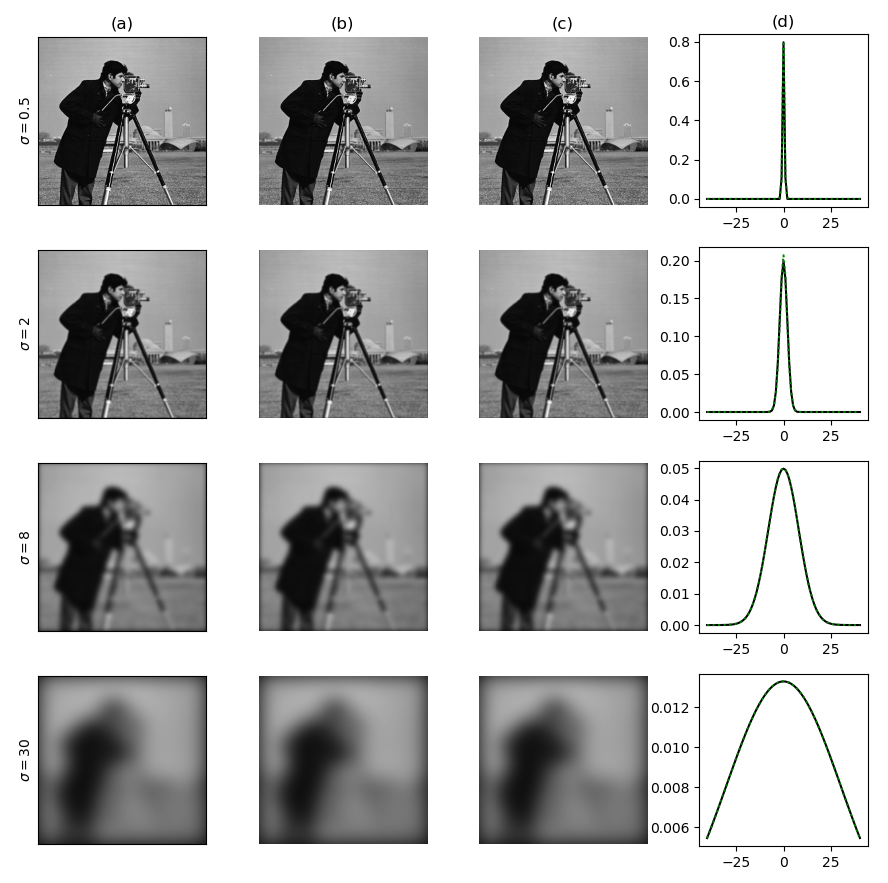
\includegraphics[width=\linewidth]{fft_gaussian_demo}
  \caption{Compatibility of Gaussian convolution strategies}
  \label{fig:fft-gaussian-demo}
\end{figure}

In \cref{fig:semigroup-demo}, we show these same three methods of Gaussian blur but for a large scale
($\sigma=45$). For each method of taking the Gaussian blur ((a) - standard convolution with sampled kernel, (b) fft with sampled kernel, (c) fft with discrete kernel), the top row is one round of Gaussian blur with $\sigma=45$ and the bottom row is two progressive passes of Gaussian blur ($\sigma_1 = 10, \sigma_2 = 35$). The mean squared error and mean absolute error between the one-pass and two-pass versions are outputted below. Code for this demo can be found in \texttt{hfft.semigroup\_demo}.
The discrete kernel performs very slightly better than the sampled versions. We originally attempted
this demonstration with a much larger sigma (say $\sigma=150$) and multiple iterations, but unfortunately multiple passes cause the ``noise'' from zeroing out around the boundaries to become very noticable after several iterations (here, we've opted to crop out a radius of pixels from around the edges equal to the standard deviation of the Gaussian before we calculated the MAE or MSE). We could show this again with a zero border or maybe even just a 1D signal.

\begin{table}
  \centering
  \begin{tabular}{c|cc}
   blurring method   & MSE & MAE \\
    \hline
spatial convolution, sampled kernel & 0.00054426 & 0.02015643 \\
FFT convolution, sampled kernel & 0.00055205 & 0.02029916 \\
FFT convolution, discrete kernel & 0.00054406 & 0.02015336
    \end{tabular}
\end{table}


\begin{figure}
  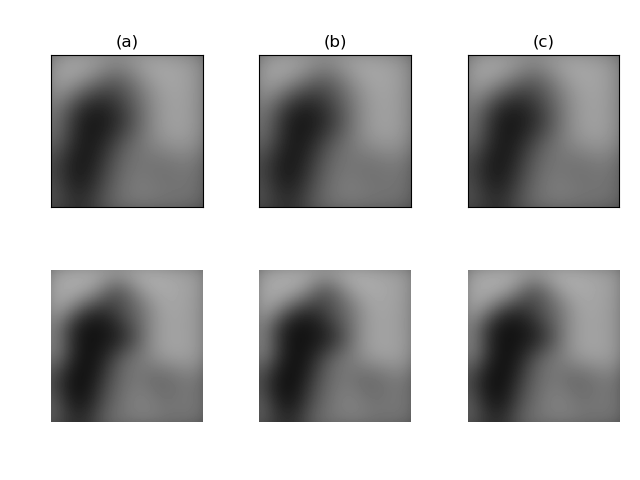
\includegraphics[width=\linewidth]{semigroup_demo}
  \caption{Iterative Gaussian blur}
  \label{fig:semigroup-demo}
\end{figure}

We further confirm the commensurate nature of Gaussian blur techniques by comparing the three techniques on a placental image and using each to calculate Frangi targets. The code can be found in \texttt{hfft\_accuracy.py}. In \cref{tab:mse-G-sigma-0.3}, \cref{tab:mse-F-sigma-0.3}, \cref{tab:mse-G-sigma-5} and \cref{tab:mse-F-sigma-5} we compare the mean squared error of a single image blurred (A) with standard spatial convolution, (B) with FFT sampled Gaussian kernel, and (C) with the discrete kernel. We see that the standard convolution and discrete convolution are very similar, while the sampled discrete Gaussian is off by two orders of magnitude, but still reasonably small. We further confirm these by viewing the intensity of the images and the Frangi targets themselves across an arbitrarily chosen horizontal cross section of the image. As seen in \cref{fig:cross-sec-G-sigma=0.3}, \cref{fig:cross-sec-F-sigma=0.3},
\cref{fig:cross-sec-G-sigma=5}, \cref{fig:cross-sec-F-sigma=5}, the peaks of the Gaussian blurred image all still occur at the same places, as do the Frangi responses. We repeated this procedure up to $\sigma=90$ and found a situation similar to $\sigma=5$; it was only in very small scales where there was any noticeable difference at all.




******************************************************************************** 


\begin{table}
  \parbox{.45\linewidth}{
  \centering
  \begin{tabular}{c|ccc}
    &  A & B & C \\
    \hline
  A & -  & 1.296e-03 & 6.772e-06 \\
  B & -  & - & 1.247e-03 \\
  C & -  &  - &  - \\
  \end{tabular}
\caption{MSE of Gaussian blurs of an image ($\sigma=0.3$)}
\label{tab:mse-G-sigma-0.3}
}
    \parbox{.45\linewidth}{
  \centering
  \begin{tabular}{c|ccc}
      &  A &  B         & C \\
      \hline
    A &  - &  4.256e-06 & 5.537e-08 \\
    B &  - &  -         & 4.337e-06 \\
    C &  - &  -         &  - \\
  \end{tabular}
  \caption{MSE of Frangi scores $\sigma=0.3$}
  \label{tab:mse-F-sigma-0.3}
}
  \end{table}



\begin{figure}
  \centering
  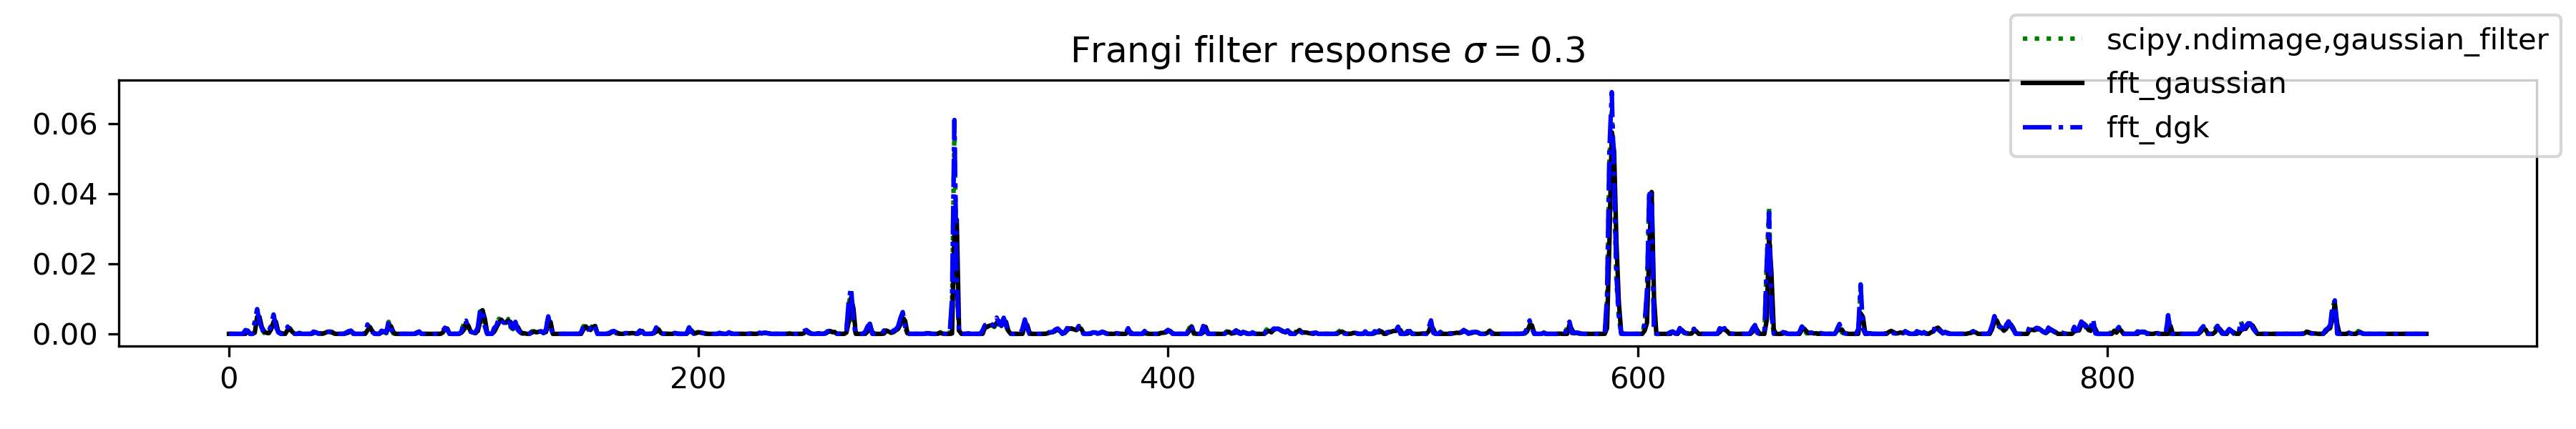
\includegraphics[width=\linewidth]{Fslice_sigma=3}
  \caption{Image cross-section of Gaussian blurred images}
  \label{fig:cross-sec-G-sigma=0.3}
\end{figure}

\begin{figure}
  \centering
  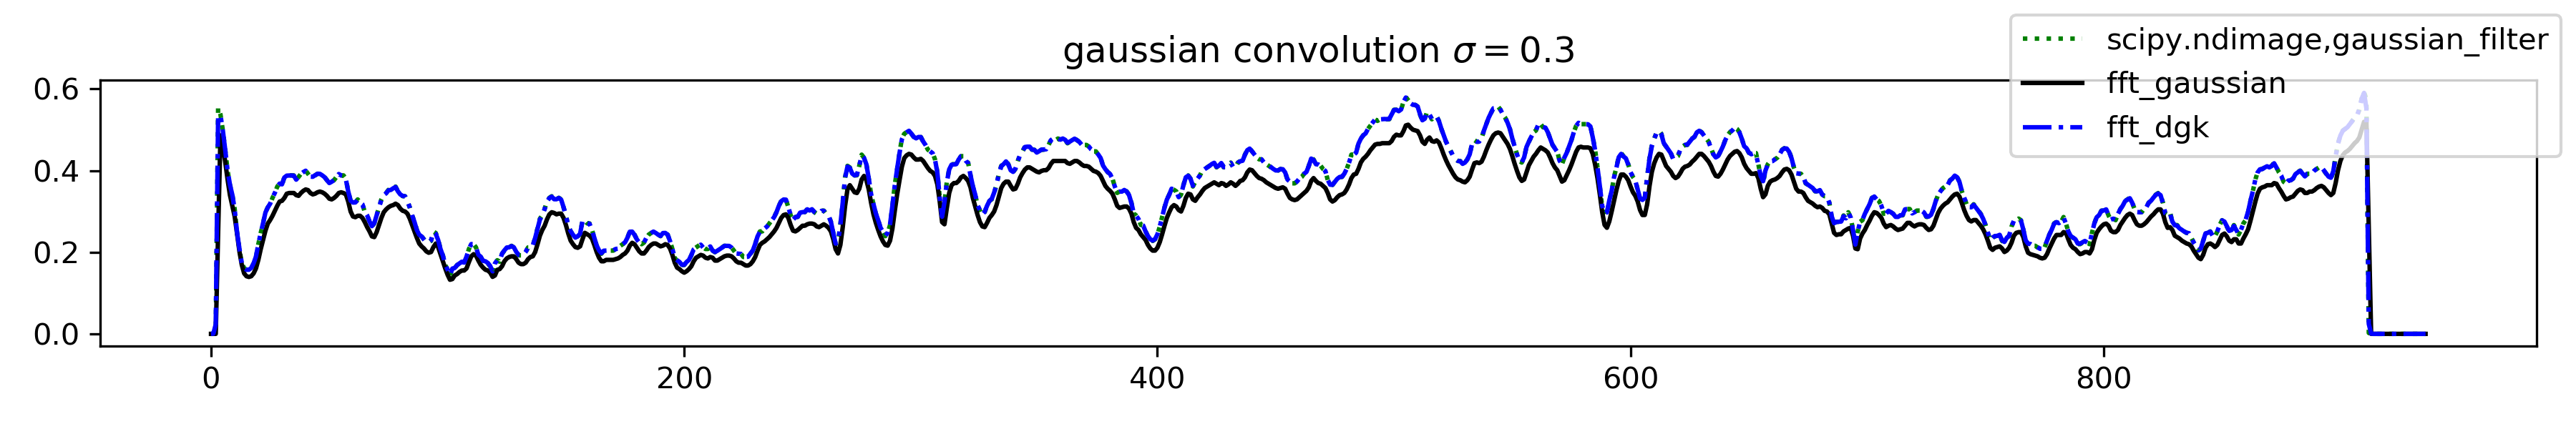
\includegraphics[width=\linewidth]{Gslice_sigma=3}
    \caption{Image cross-section of Frangi targets images}
    \label{fig:cross-sec-F-sigma=0.3}
\end{figure}



\begin{table}
  \parbox{.45\linewidth}{
    \centering
    \begin{tabular}{c|ccc}
      &  A & B & C \\
      \hline
      A & -  &  9.012e-06 & 8.629e-09 \\
      B & -  & - & 9.031e-06 \\
      C & -  &  - &  - \\
    \end{tabular}
    \caption{MSE of Gaussian blurs of an image ($\sigma=5$)}
    \label{tab:mse-G-sigma-5}
  }
  \parbox{.45\linewidth}{
    \centering
    \begin{tabular}{c|ccc}
      &  A &  B         & C \\
      \hline
      A &  - &  9.388e-05 8.383e-07 \\
      B &  - &  -         & 9.599e-05 \\
      C &  - &  -         &  - \\
    \end{tabular}
    \caption{MSE of Frangi scores $\sigma=5$}
    \label{tab:mse-F-sigma-5}
  }
\end{table}

\begin{figure}
  \centering
  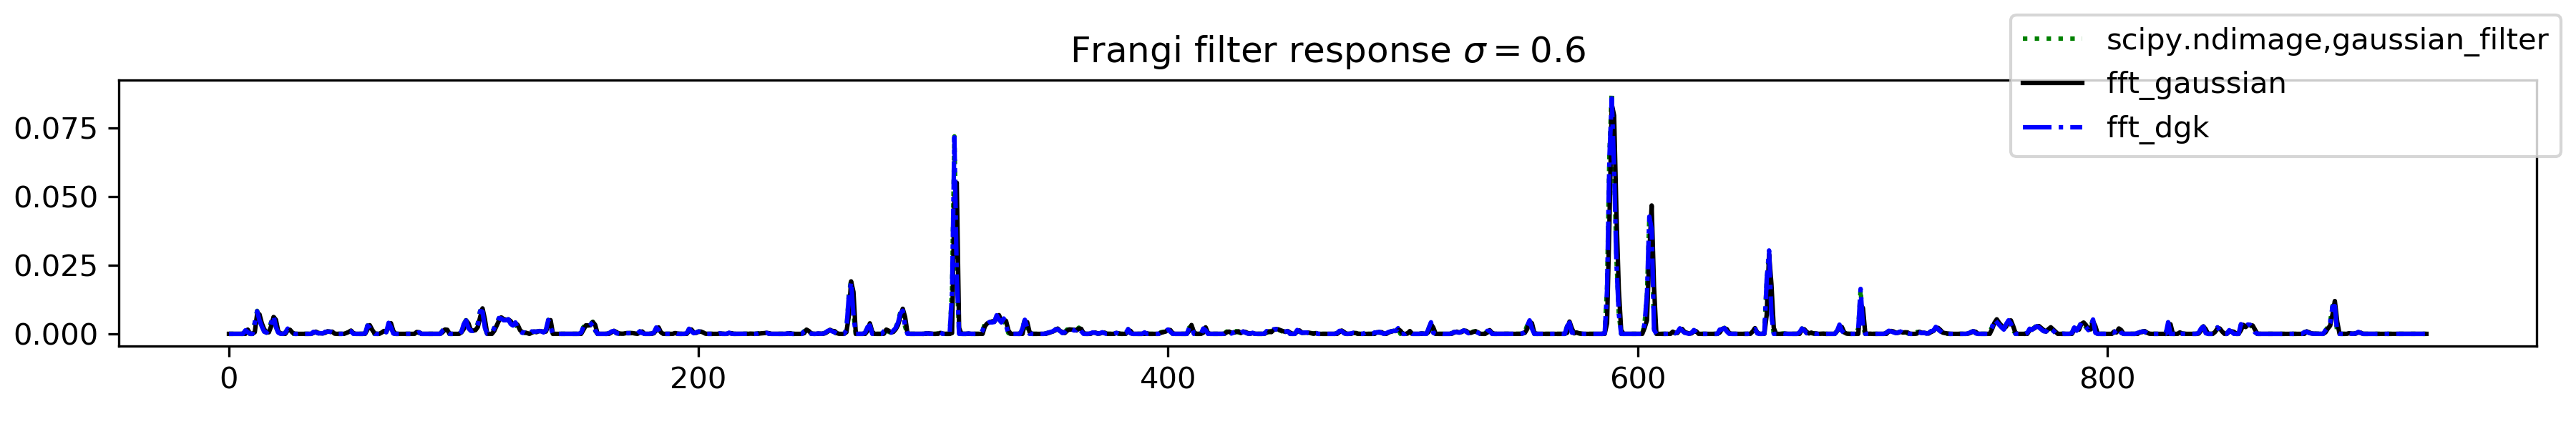
\includegraphics[width=\linewidth]{Fslice_sigma=6}
  \caption{Image cross-section of Gaussian blurred images $\sigma=5$}
  \label{fig:cross-sec-G-sigma=5}
\end{figure}

\begin{figure}
  \centering
  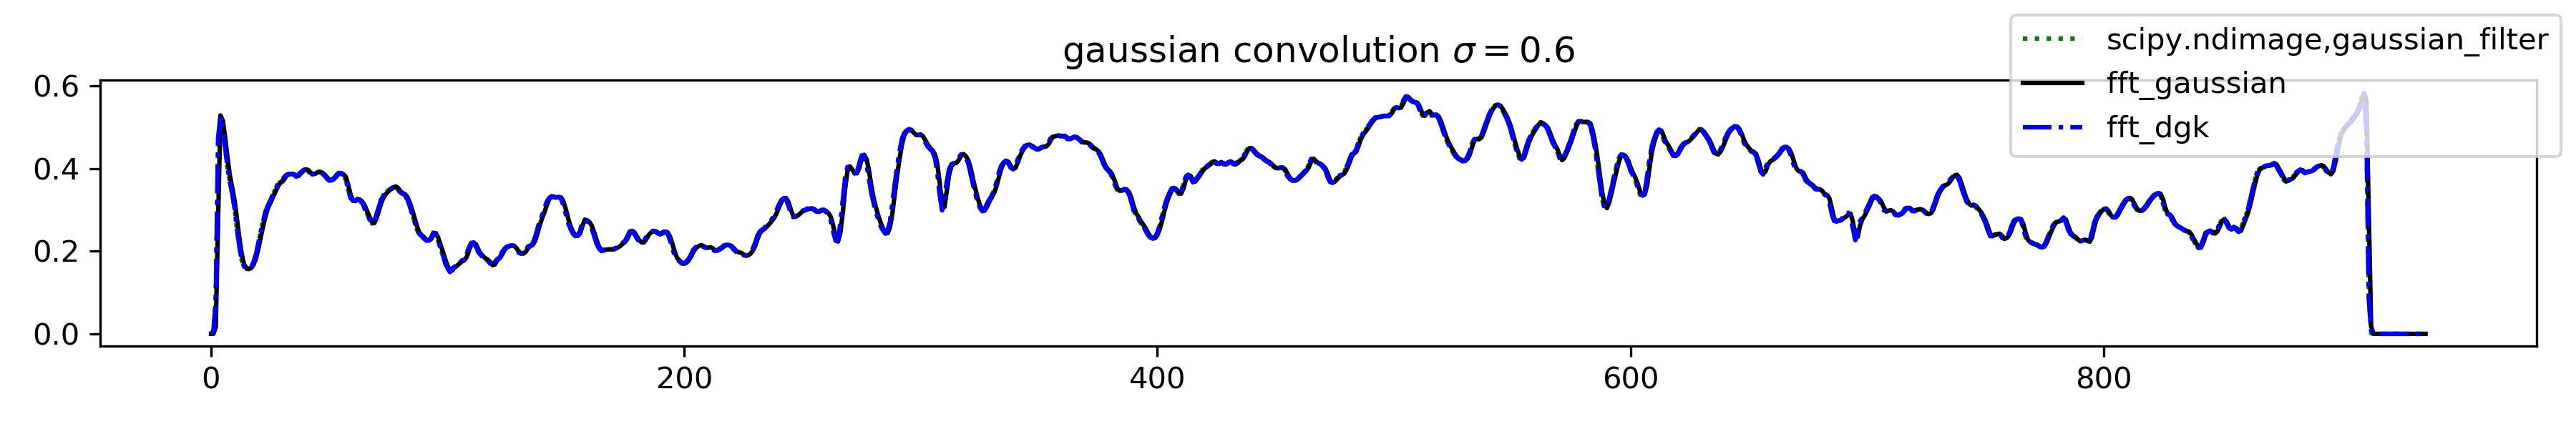
\includegraphics[width=\linewidth]{Gslice_sigma=6}
  \caption{Image cross-section of Frangi targets images $\sigma=5$}
  \label{fig:cross-sec-F-sigma=5}
\end{figure}


Finally, we wish to demonstrate the point of this comparison--that $FFT-based$ convolution is much faster than spatial convolution. We took a much larger sample ( 2200 by 2561) and timed each method of convolution (average of three trials) for a large number of samples: logarithmic between $\sigma=1$ and $\sigma=128$ with 32 steps. The result shows that the convolution time seems to at least linearly increase with the size of the kernel, whereas fft convolution behaves independently.

Frangi filtering

\begin{figure}
  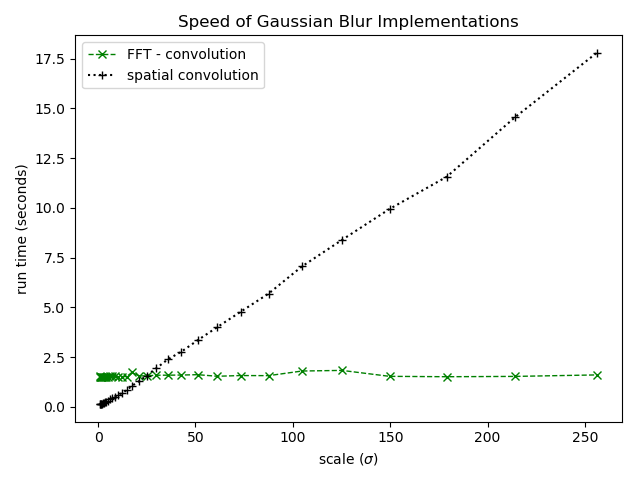
\includegraphics[width=\linewidth]{convolution-runtime-demo}
  \caption{Time required}
\end{figure}
\chapter{Research Protocol} \label{ch:research-protocol}

We ultimately perform a multiscale Frangi prefilter on a subset of 201 color images of placental samples. We describe here the sample set and the preprocessing steps we take prior to performing the multiscale filter.

\section{Samples / Image Domain}\label{sec:NCS-data-set}

The 201 samples are from a larger private database provided by the National Children's Study, which had been prepared for a different study \cite{chang2017}. These 201 samples are those that have a ground truth provided, although the actual database is much larger with many untraced samples. The placental samples were cleaned and formalin-fixed prior to their being photographed \cite{almoussa-ucla-reu}, and their placental chorionic surface vascular networks (PCSVN) manifest as primarily dark curvilinear structures. The samples are provided as XCF files (the native project file for the image processing software GIMP) and contain four major layers.

\subsection{A Representative Sample}
The layers together give a hand tracing of the vascular network and perimeter. A sample of overlaid layers in a representative sample (with ID number ``BN0164923'') is given in \cref{fig:NCSlayers}.

\begin{figure}[p] \centering
    \subfloat[Fixed Placental Sample]{        \label{fig:NCSlayers-raw}\includegraphics[width=80mm]{{{T-BN0164923.raw}}}
        }
    \subfloat[Perimeter tracing and UCIP]{
        \label{fig:NCSlayers-P}\includegraphics[width=80mm]{{{T-BN0164923_perimeter_overlay}}}
    }\
    \subfloat[Arterial tracing]{
        \label{fig:NCSlayers-A}\includegraphics[width=80mm]{{{T-BN0164923_arteries_overlay}}}
        }
    \subfloat[Venous tracing]{
        \label{fig:NCSlayers-V}\includegraphics[width=80mm]{{{T-BN0164923_veins_overlay}}}
        }\
    \subfloat[Total Vascular Network]{
        \label{fig:NCSlayers-T}\includegraphics[width=80mm]{{{T-BN0164923_all_layers_overlay}}}
        }
    % should i use the real sample names? or obfuscate?
\caption{A representative placental sample and tracing}
\label{fig:NCSlayers}
\end{figure}

Each sample is roughly 1954x1200 pixels with some occasional variation.
In \cref{fig:NCSlayers}, we see these four layers of a characteristic sample.
\cref{fig:NCSlayers-raw} is the base image.
A cleaned, formalin-fixed placenta is placed on a table with a camera a fixed distance away,
and a ruler and penny (presumably for redundancy) are placed nearby to aid registration and
calibration of the resolution.
The resolution of each sample is roughly 46 pixels per centimeter, with some variation.
\cref{fig:NCSlayers-P} is a tracing (in green) of the perimeter of the placenta.
The umbilical cord insertion point (UCIP) is notated in yellow.
Two cyan marks are placed on consecutive centimeter markings on the ruler.
The dots are enlarged and shown as a darker blue in the figure for clarity.
\cref{fig:NCSlayers-A} and \cref{fig:NCSlayers-V} are each hand traces of the PCSVN,
  with a layer for each the arteries and veins.
These layers are simultaneously overlain on the base image in \cref{fig:NCSlayers-T},
with the arterial trace on top,
just as the arteries generally lay on top of the veins in the samples themselves.
In these traces, the coloration of each vessel corresponds its the reported diameter.
The diameters are binned into 9 discrete widths, odd integers from 3 to 19 pixels.
Vessels of smaller diameter are either binned to three or (quite frequently) left untraced.
The correspondence between pencil color and (binned) vessel width used in the tracing protocol
  is given in \cref{tab:widthcolors}.

\begin{table}
    \centering
\begin{tabular}{ccc}
    \hline
    \rule[-1ex]{0pt}{2.5ex}
    vessel width & color (hex value) & approximate color \\
    \hline 
    \rule[-1ex]{0pt}{2.5ex}
    3 pixels &  \texttt{\#ff006f} &   magenta \\                                      
    \rule[-1ex]{0pt}{2.5ex}
    5 pixels & \texttt{\#a80000}  & dark red \\                                      
    \rule[-1ex]{0pt}{2.5ex}
    7 pixels &  \texttt{\#a800ff} & purple \\                                          
    \rule[-1ex]{0pt}{2.5ex}
    9 pixel s&  \texttt{\#ff00ff}  & light pink \\
    \rule[-1ex]{0pt}{2.5ex}
    11 pixels &  \texttt{\#008aff} & blue \\                                          
    \rule[-1ex]{0pt}{2.5ex}
    13 pixels &  \texttt{\#8aff00} &   green \\                                        
    \rule[-1ex]{0pt}{2.5ex}
    15 pixels &  \texttt{\#ffc800} &  gold \\                                    
    \rule[-1ex]{0pt}{2.5ex}
    17 pixels & \texttt{\#ff8a00}  &  orange \\                                         
    \rule[-1ex]{0pt}{2.5ex}
    19 pixels & \texttt{\#ff0015}   &  bright red  \\
    \hline
\end{tabular}
\caption{Vessel Width Color Code for Manual Tracing Protocol}
\label{tab:widthcolors}
\end{table}


The task of creating these samples, in particular the tracing and estimation involved in creating \cref{fig:NCSlayers-A} and \cref{fig:NCSlayers-V} is very labor intensive--requiring between 4 and 8 hours to trace a single sample.
A closer look at many of the samples often reveals that a great deal of subjectivity in providing this ``ground truth,'' as it is not often clear what the underlying truth really is. Often it's hard to see where the vein is, vascular networks are obscured by the umbilical stem, the blood in the vessels dries unevenly or ruptures, and the vessel seems to disappear momentarily. These situations and more will be discussed in \cref{sec:NCS-dataset-issues}, where we will demonstrate how the Frangi filter reacts to these problem areas. Our efforts at the eventual task of total network completion must deal with these shortcomings and, in some circumstances, make subjective decisions like the manual tracer did.


\subsection{Knowns and Unknowns}
Since our final goal is a fully automated procedure, we wish to simply operate on the placental sample itself, without any understanding of its provided tracing (except for judging the strength of our algorithm);
our goal is to develop an algorithm that can produce a ``ground truth'' tracing similar to \cref{fig:NCSlayers-T} or \cref{fig:NCSoutput-trace} without any user intervention.

For our purposes however, we will concede and provide a limited amount of information from the tracings, namely the provided placental perimeter (shown in green in \cref{fig:NCSlayers}). In \cref{sec:perimeter-detection} we will describe a simple edge finding algorithm that allows us to estimate the perimeter in \cref{fig:NCSlayers-P}.
Unfortunately we achieve a subpar result on a small subset of images--roughly 7 of the 201 total images--using our currently implemented algorithm, and in such cases will revert to using the reported perimeter from the ground truth.

%to provide which were previously reported as being inside the plate and sometimes led to large false positives. In the case that this method 
%In developing a fully automated algorithm, it would be relatively straightforward to obtain this boundary ourselves using various techniques, such as an Active Contour Model \cite{activecontours} or, even 
%We do use the traced placental perimeter at our own peril, however, since often there are tears in the side of the plate or large amounts of non-vascular content with large changes in height that are not adequately accounted for in the perimeter tracing.

Finally, we will consider the location of the umbilical insertion point as a ``known'', as the vessels around it are frequently impossible to see and we wish to exclude them from consideration. It is not unreasonable, however, to consider this to be a known--in future preparations of samples, we could simply require that this point be centered in image in a predictable location prior to the picture being taken.
Furthermore, we suggest that we can avoid this in the future by using an algorithm to find the umbilical cord stump and mask that region. Such an algorithm is certainly reasonable, although we were not able to implement something that worked on all images in a uniform fashion. Noise from the umbilical stump, if not addressed, will affect the fidelity of our filter. We will discuss this further in \cref{sec:NCS-dataset-issues}.

\section{Data Cleaning and Preprocessing}

Building a sample suitable for use in our algorithm from \cref{fig:NCSlayers} is relatively simple. We  zero  outside the boundary of the plate (so as to not waste computational time calculating the differential geometry of a ruler, say), and also generate a binary mask to identify the plate. Finally, our vessel layers are combined and given as a binary trace, which we will use later for scoring. An example of the preprocessed samples used by the algorithm are given in \cref{fig:exampleNCSoutput}.

These procedures are performed automatically on the 201 images in our data set using a custom GIMP plug-in, which performs various ``bucket fill'' operations, layer mergings, and thresholdings.
%For completeness sake, this plug-in (and an associated Scheme script which turns it into a batch operation) can be found in the Appendix.

\begin{figure}\label{fig:exampleNCSoutput}     \centering
    \subfloat[Background mask (in white)]{
        \label{fig:NCSoutput-mask}\includegraphics[width=80mm]{{{T-BN0164923.mask}}}
    }
    \subfloat[Sample with background removed]{
        \label{fig:NCSoutput-base}\includegraphics[width=80mm]{{{T-BN0164923}}}
    } \\
    \subfloat[Grayscale]{
        \label{fig:NCSoutput-gray}\includegraphics[width=80mm]{{{T-BN0164923.L}}}
    }
    \subfloat[Trace / ``Ground Truth'']{
        \label{fig:NCSoutput-trace}\includegraphics[width=80mm]{{{T-BN0164923.trace}}}
    }
    \caption{Preprocessed files from an NCS sample}
\end{figure}

    As a point of technicality, the grayscale image in \cref{fig:NCSoutput-gray} is not actually produced directly by the extractor plug-in, but created when the 3 channel RGB image \cref{fig:NCSoutput-base} is imported at the start of the algorithm. This grayscale conversion is simply done for ease of analysis on the sample: although the Frangi filter is designed for arbitrary $N$-dimensional input \cite{frangi-paper}, an image with three color channels does not have 3 spatial dimensions. We therefore simply combine the information in three channels using the well-known and oft-implemented ITU-R 601-2 luma , or ``luminance'' transform \cite{scipy}:
    
    \begin{equation} \label{eq:luma_transform}
    L =  \frac{299}{1000}\ R + \frac{587}{1000}\ G + \frac{114}{1000}\ B
    \end{equation}
    It should be noted that this choice is not requisite--several other attempts have opted to use the image's green channel instead \cite{almoussa-ucla-reu} and \cite{huynh2013filter}. Preliminary and periodical rechecking has not indicated that such a conversion has any benefit over the luminance transformation for our image domain, although other placental samples with a different preparation method or color profile might benefit from it.

\subsection{Placental Perimeter Detection and Background Masking} \label{sec:perimeter-detection}
\begin{figure}     \centering
  \subfloat[Raw (traced mask)]{
    \includegraphics[width=0.24\textwidth]{{{cut_demo_new_cimg_gt}}}
  }
  \subfloat[Raw (watershed mask)]{
    \includegraphics[width=0.24\textwidth]{{{cut_demo_new_cimg_ws}}}
  } %\\
  \subfloat[$\Vmax$ (traced mask)]{
    \includegraphics[width=0.24\textwidth]{{{cut_demo_new_f_gt}}}
  }
  \subfloat[$\Vmax$ (watershed mask)]{
    \includegraphics[width=0.24\textwidth]{{{cut_demo_new_f_ws}}}
  }\\[12pt]
  \caption{Automated placental perimeter detection}
  \label{fig:cut-demo}
\end{figure}

As mentioned above, expect for a few small images, we estimate the perimeter of the placental plate from the raw image, rather than using the ground truth's traced perimeter. Most notably, the placental plate often includes includes a small V-shaped cuts in the placental plate.
The traced placental perimeter often overlooks these regions and opt for a more convex shape.
In \cref{fig:cut-demo}, we showcase the effect of using our automated approach versus using the ground truth mask. The first two images demonstrate the Notably, this prevents the white background leading to false positives at the edge of the cut.
To find the placental plate,we take the gradient of the raw sample's green channel with a very small scale $\sigma=.01$ to identify very small and sharp edges. We then mark the top right pixel, which is certainly outside the placental plate, with a background marker, and we label any points where the gradient is above its mean value as foreground. We then perform a watershed of the gradient given these markers and then perform a binary erosion of the result with radius 15 to regularize the result \cite{skimage} \cite{DIPGW}. From this, we grab the largest foreground object, which will inevitably be the placental plate. Unfortunately, there are 7 of the 201 samples for which this procedure fails, typically due to poor contrast at the edge of the placental plate. In the case of these samples, we revert to simply using the traced outline of the placenta as given by the tracing protocol.

    \subsection{Boundary Dilation} \label{sec:boundary-dilation}
    
    All images are grayscale, $M,N$ pixels as a masked array (of type
    \textrm{numpy.ma.MaskedArray}), where pixels outside of the placental region are masked so they will not be considered by the algorithm. However, some standard
    implementations of algorithms, namely \textrm{numpy.gradient and scipy.signal.convolve2d} are not designed to handle masked regions. Although it would be potentially useful to adapt such methods in a way to, say, calculate a gradient or perform a convolution by a ``reflection'' across an arbitrary closed boundary (as opposed to the edge of the image matrix), we opted instead to ``zero out'' unwanted background pixels and simply exclude affected areas from consideration. This exclusion could be achieved by
    simply dilating the mask, but we opt to achieve it in a much more resource efficient manner: we iterate through an array of indices for the image where the boundary occurs and simply extend the mask $R$ pixels in each direction (like a giant plus sign). Since the boundary of the placental plate forms a closed loop, the effect is very similar to convolving with a disk of radius $R$, but is much faster.
    
    \begin{figure} 
        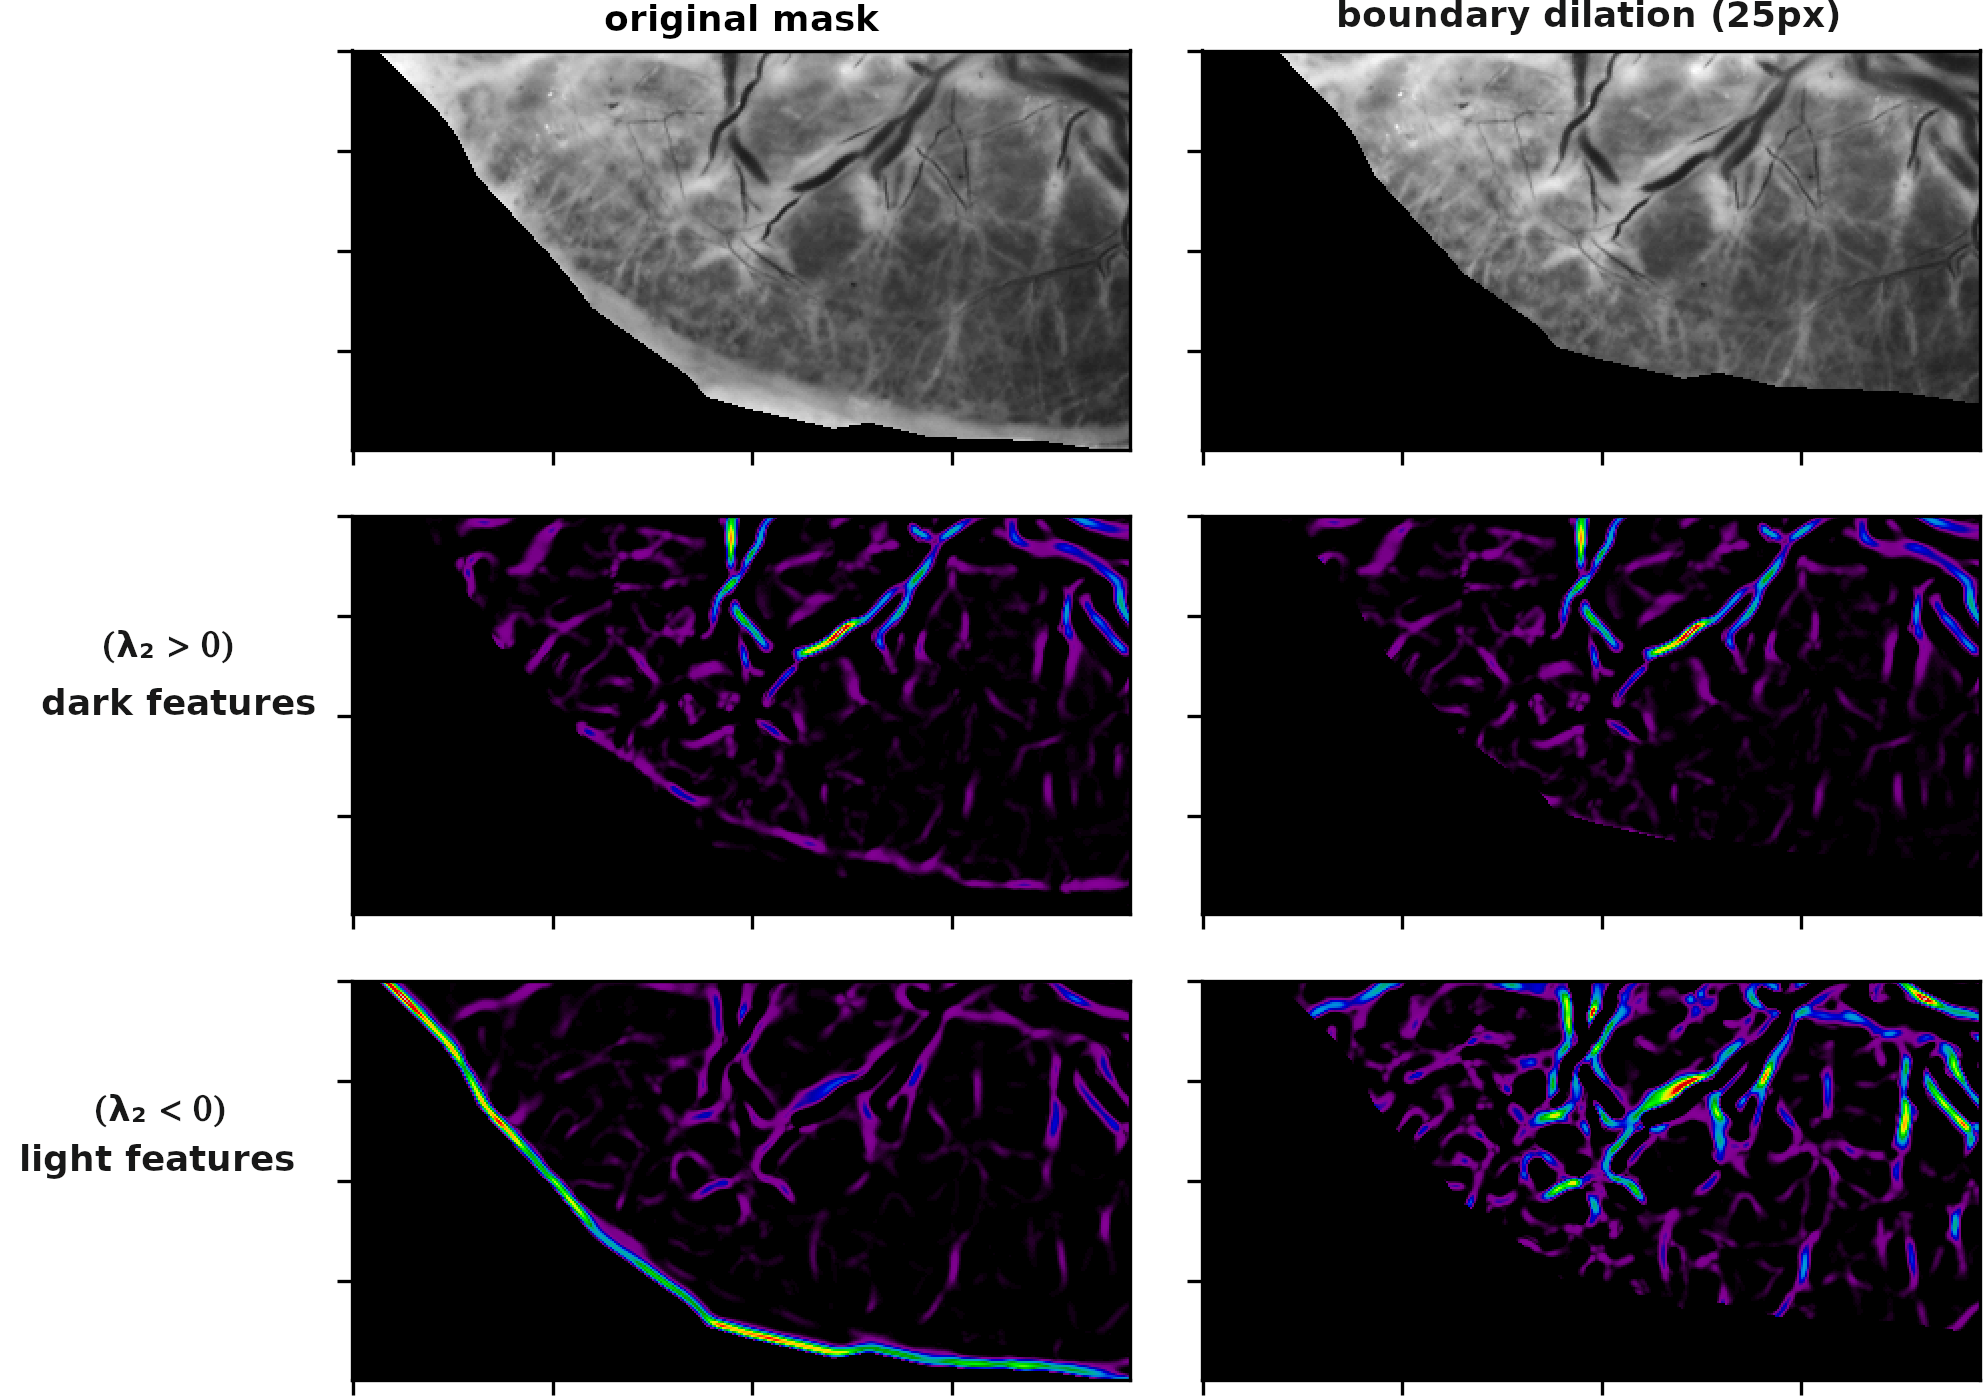
\includegraphics[width=\textwidth]{boundary_dilation_demo_labels}
        \caption{Effect of boundary dilation on Frangi responses}
        \label{fig:boundary-demo}
    \end{figure}
    
    \cref{fig:boundary-demo} shows the effect of this so-called ``boundary dilation.'' 
    We show the output of the Frangi filter with $\sigma=3$. A border radius of $25$ is chosen to exaggerate the effect.
    The first row shows the unaltered boundary of the sample (left) and
        the sample after boundary dilation (with radius dilation of 25 pixels).
    The second row shows the Frangi vesselness measure at single scale ($\sigma=3$) where \textrm{DARK\_BG=False} to target dark curvilinear structures performed on the altered sample (left) and the boundary dilated sample (right). Removing an unnecessary part of
    the placental plate prevents a small response to a non-vascular yet mildly curvilinear
    background feature from appearing.
    The third row of \cref{fig:boundary-demo} shows the Frangi vesselness measure at the same scale ($\sigma=3$) when we are probing for bright curvilinear structures (i.e.
    \textrm{DARK\_BG=True}). Here, wherever the very edge of the placental plate is *any* brighter than adjacent interior, a very large Frangi response will occur, as seen on the left. Dilating the boundary completely avoids this issue, as seen by the figure on the right. Thus we prevent a visual artifact that is present in much prior work on this problem \cite{huynh2013filter,almoussa-ucla-reu}.

    It should be noted that, while the figure on the right shows a much larger interior response, this is simply because the intensity of the output in each of these
    images is being independently scaled between the minimum and maximum intensity in the image. However, we argue that this is an appropriate and desired depiction of the situation, as we will frequently consider only the relative maxima of Frangi response per scale in our analysis.
    
    We end our discussion by noting that we perform this boundary dilation within the
    Frangi algorithm itself when we set the structureness parameter $\gamma$ as half of the maximum Hessian norm found at that scale--this ensures that the maximum occurs sufficiently away from the boundary of the plate, and does not occur from a noise phenomenon.

    
    
%    Sometimes there are small cuts that appear on the side of the placental plate, which can lead to large filter responses. We would like to filter these out to eliminate false positives in any way we can. These places are identified somewhat reliably by the tracing protocol with a blue dot. We perform a morphological watershedding in this area in an attempt to add this area to the mask.
%    The threshold for the watershed is ultimately based on the background value of the blue dot; if this is incorrectly placed (or anything else weird happens), we can manually opt to simply remove a large area from consideration from the plate, as we do the umbilicial cord insertion point. This is demonstrated in \cref{fig:cutdemo}. From left to right, we have the original masked placental sample, the cut mark notated on the perimeter layer, the improved mask after watershedding, and finally, the ``scorched earth'' approach in case the previous attempt failed. In few additional cases, neither approach is adequate. We again will stress that a fully automated algorithm would have no knowledge of our traced perimeter (as in \cref{fig:NCSlayers-P} or the second from left image in \cref{fig:cutdemo}), so we anticipate a fully automated method of handling that problem should also be able to correct for these ``cuts'' as well.
%    
%    \begin{figure}
%        \centering
%        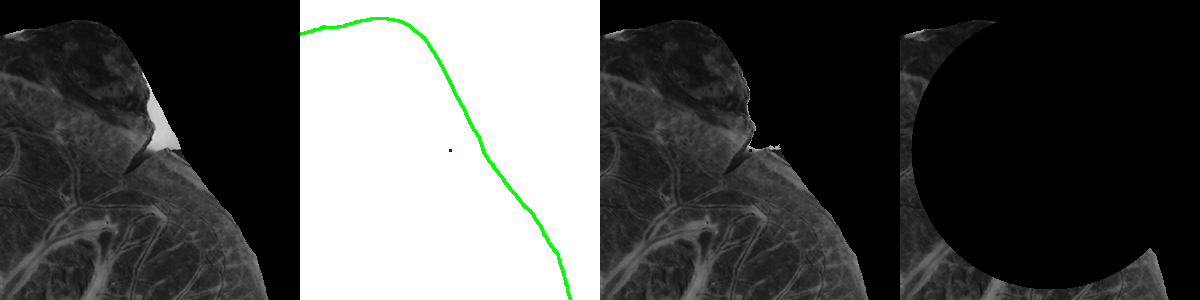
\includegraphics[width=\linewidth]{T-BN0342010_cutopts}
%        \caption{Removing a ``cut'' from the placental plate.}
%        \label{fig:cutdemo}
%    \end{figure}
    
%    \subsection{Finding Placental Border}
%		
%		We take the gradient of the sample green channel of the raw sample with a very small scale $\sigma=.01$ to identify very small and sharp changes. We then mark the top right pixel, which is certainly outside the placental plate, with a background marker, and we label any points where the gradient is above its mean value as foreground. We then perform a watershed of the gradient given these markers and then perform a binary erosion of the result with radius 15 to regularize the result. From this, we grab the largest foreground object, which will inevitably be the placental
%		plate. Unfortunately, there are 7 of the 201 samples for which this procedure fails. In the case of these samples, we revert to simply using the traced outline of the placenta as given by the tracing protocol.
		
		    \subsection{Deglaring}
    
    Despite best efforts when harvesting samples, a select number of the placental samples exhibit substantial glare, which leads to inaccuracies in identifying curvilinear content. Our protocol for deglaring is analogous to that performed in \cite{almoussa-ucla-reu} and \cite{huynh2013filter}. Unfortunately, the method relied upon by those previous papers (\textrm{MATLAB}'s \textrm{imfill}, which relies on inpainting by solving the Dirichlet problem for masked regions) was not immediately available in a Python environment. Instead, we used an already implemented inpainting algorithm, \textrm{scikit-image}'s \textrm{inpaint\_biharmonic()}, which should be expected to achieve similar results, albeit at the expense of processing time.
    
    The function \textrm{inpaint\_biharmonic} is based on \cite{damelin2018surface}, and relies on solving the biharmonic equation i.e. $\nabla \nabla f = 0$
    for the surface $f$ subject to boundary conditions (as
    compared to \textrm{imfill}'s solving the Laplace equation $\nabla f = 0$ in regions marked as glare.
    
    The method for deciding what is considered glare is similar to \cite{almoussa-ucla-reu}, in which we
    consider any intensities close the maximum intensity in the image (Almoussa et al. used $80\%$ of max intensity, and we use $175/255 \approx 68\%$). This threshold is unfortunately dependent on the image domain.
    
        \begin{figure} 
        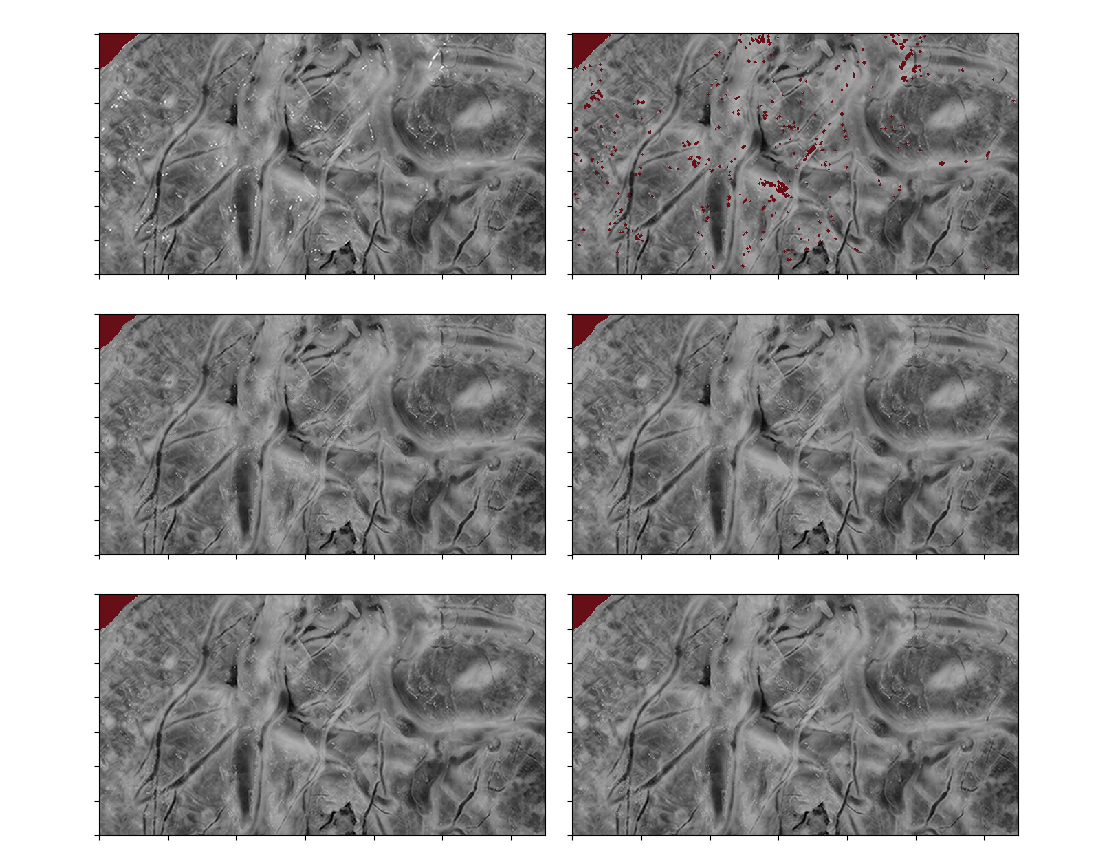
\includegraphics[width=\textwidth]{preprocessing_comparison_cropped_fig}
        \caption{Deglaring a sample using a hybrid inpainting method}
        \label{fig:glare-example-crop}
        \end{figure}

        \begin{figure}[t] \centering
        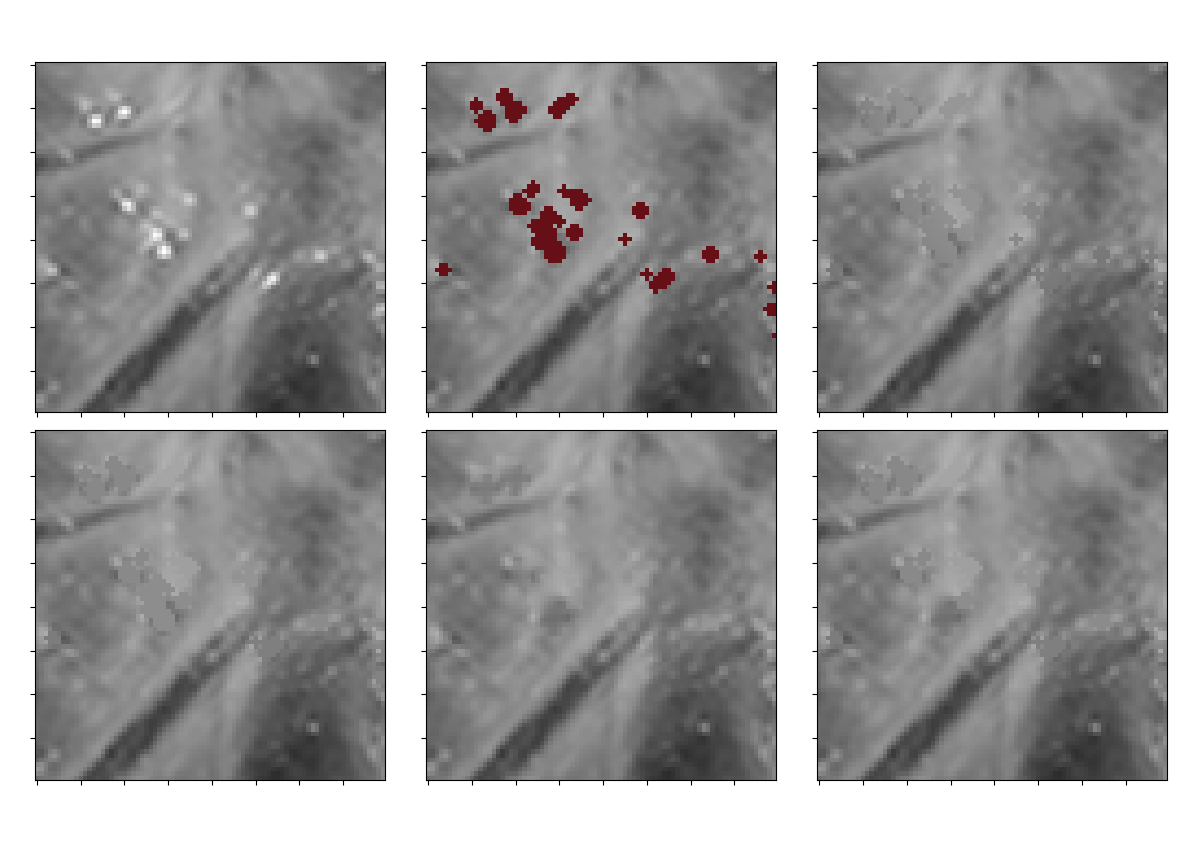
\includegraphics[width=0.8\textwidth]{preprocessing_comparison_zoomed_fig}
        \caption{Comparison of glare inpainting methods (detail)}
        \label{fig:glare-example-zoom}
        \end{figure}
    
    Inpainting in the above way is rather resource intensive, so we implemented two faster and less precise methods of inpainting that work well enough for removing small regions of glare.
    These methods can be found in \textrm{preprocessing.py}. The first, called 
    \textrm{inpaint\_glare()}, replaces any masked pixel with the average of all non-masked values within a certain distance (default 15 pixels). The second, called \textrm{inpaint\_with\_boundary\_median} calculates the median value of the  (non-masked) boundary and fills any masked region with that value. We argue that these less-exact methods are adequate for smaller regions, while larger regions of glare deserve a more thoughtful application of inpainting. Our final method of inpainting, \textrm{inpaint\_hybrid} implements this idea--smaller glare regions are inpainted with a boundary median, while larger areas are inpainted with the more expensive but more accurate biharmonic inpainting.
    
    A comparison of these methods is shown in \cref{fig:glare-example-crop},
    and a zoomed in portion is shown in \cref{fig:glare-example-zoom}.
    In the top left of each, the glary image is shown.  In the top middle,
    regions above the threshold intensity are masked (shown in dark red, along with the background). In the top right, the strategy is ``mean window'' with a window size of 15 pixels. The bottom left uses ``boundary median'' strategy. The middle is the more expensive ``biharmonic inpainting'' strategy, and the bottom right uses a ``hybrid'' strategy.
    
    The following timing demonstrates that the ``hybrid'' strategy is over 3 times faster than biharmonic inpainting, and that biharmonic painting takes 22 seconds, even when only 1\% of the placental plate is to be inpainted.
    
    Inpainting with boundary median only four seconds, inpainting all sections with the biharmonic method took 22 seconds, and a hybrid method took 6.5 seconds. Roughly 1 percent of nonmasked pixels in the image were inpainted.

%    \begin{lstlisting}
%    In [1]: %timeit inpaint_with_boundary_median(img)
%    1 loop, best of 3: 3.99 s per loop
%    
%    In [2]: %timeit inpaint_with_biharmonic(img)
%    1 loop, best of 3: 22.3 s per loop
%    
%    In [3]: %timeit inpaint_hybrid(img)
%    1 loop, best of 3: 6.49 s per loop
%    
%    In [4]: px_inpainted = np.sum(np.logical_and(masked.mask, np.invert(img.mask)))
%    In [5]: px_plate = np.sum(np.invert(img.mask))
%    In [6]: px_inpainted / px_plate  # ratio of inpainted pixels to total plate 
%    Out[6]: 0.011444460505513942
%    \end{lstlisting}

    
    We stress again that only a small subset our image domain exhibits disruptive amounts of glare for anything except small scales. Future improvements in this direction should probably seek to implement more robust method such as \cite{lange2005glare} that are not dependent on an arbitrary global
    threshold for deciding what regions exhibit glare.
    
    
\section{Multiscale Setup}

    Our multiscale Frangi filter requires a list of scales at which to probe. Each scale is chosen to accentuate features (i.e. vessel diameter) of a particular size.
    This set of scales at which to probe will be denoted as $\Sigma := \{ \sigma_1, \sigma_2, \dots, \sigma_N\}$, where each scale in indexed by increasing order.
    
    Although we cannot expect \textit{a priori} that there is an direct proportionality between our scale size $\sigma$ and (even some function of) the width of a particular vessel \cite{frangi-paper}, we generally expect to isolate
    narrower curvilinear structures at smaller scales, and thicker curvilinear structures at larger scales.  The smallest one should be an effective size where details are expected to be isolated, and the largest should be an effective size as well. In fact, following \cite{Koenderink}, it is reasonable and natural to select these logarithmically; that is, for some selected inputs $m < M$ we have
    
    \begin{equation}
    \sigma_1 = 2^{m} \; , \; \cdots \; , \; \sigma_{j} = 2^{\left(m+\frac{M-m}{N-1}j\right)} \; , \; \cdots \; \sigma_N = 2^{M} \end{equation}
    
    That is, the exponents are spaced linearly from $m$ to $M$. This is achieved by the command
    \textrm{np.logspace(m,M,num=N)}. The idea is that the curvilinear content of the image will respond better at some particular scale, but there are diminishing returns as $\sigma$ increases; while the filter's response may vary substantially between, say $\sigma=1$ and $\sigma=2$, we would not expect a substantial difference in response between, say, $\sigma=46$ and $\sigma=47$. Historically, there was another benefit of using a logarithmic scale space: computing the vesselness measure was very expensive, and thus it was simply not feasible to collect so many large scale readings. This is much less of an issue with the present implementation, although we still obviously wish to avoid frivolous, redundant calculations no matter the speed of the implementation.
    
    The optimal choice of scale sizes to probe at is intuitively dependent on the resolution of the image. If there is no particular care taken in selecting a minimum and maximum scale at which to probe, then we must assure that our Frangi filter is ``normalized'' in such a way that there is a decay in response past certain values. That is, probing at a unreasonably large (or small) scale--say $\sigma=1000$ or $\sigma=.0001$--should result in an almost null response throughout the image. We will approach this issue in our discussion of ``variable thresholding.'' 
    
    \section{The Research Protocol}
    Once we have chosen this set of scales $\Sigma$, we simply convolve the image with a discrete Gaussian kernel with that standard deviation, then take gradients enough to get a matrix of partial second derivatives, the Hessian. We calculate the eigenvalues of each (2x2) Hessian matrix and then compute the Frangi filter according to \cref{ch:unifrangi} and \cref{ch:multifrangi}. We use these to provide a couple examples of estimating the PCSVN network. The entire decision tree can be shown in the outline below. We follow the procedure for \cref{ch:segmentation}. For our analysis of the Frangi filter apart from segmentation we shall stop before step (C).
    
    \begin{spacing}{1}
    \begin{small}
    \begin{verbatim}
For each sample:

A) Preprocessing
  1) Find placental border
  	a) Gradient of green channel for small sigma=.01
  	b) Watershed outside against above gradient mean
  	c) erode these points, radius=15
  	d) Identify largest object in watershed threshold
  2) RGB to single channel via Luminance Transform
  3) Glare removal
    a) Mask glare (threshold at *175/255*)
    b) Dilate glare mask with radius=2
    c) Inpaint glare
      + Hybrid inpainting, with size threshold *32*
      . Biharmonic inpainting
      . Median value of boundary
  4) Dilate around UCIP, add to mask (radius=50)
B) Multiscale Frangi filter
  1) Set parameters
    a) Scales
      = n_scales (default: *20*)
      = log_range (default *[-1.5, 3.2]*), log base 2
      -> scales
    b) Beta = 0.1, Gamma = 1.0 (or alternate parametrization)
    d) Dilate mask per scale (20 pixels)
  2) For each sigma: compute Uniscale Frangi Filter
    a) gauss blur image with discrete Gaussian kernel FFT
    b) take gradient across each axis of blurred image;
       take gradient across each axis of gradient
       -> (Hxx, Hxy, Hyy)
    c) Find eigenvalues of hessian at each point (using np.eig)
       and sort by absolute magnitude 
    d) Calculate Frangi Vesselness Measure
  3) Split positive and negative strain.
  3) Merge each result, reserve positive and negative stacks
C) Estimate PCSVN
  1) Approximate using strategy
    a) Calculate Vmax above high fixed threshold alpha=0.3
    b) Calculate Vmax above lower fixed threshold alpha=0.2
    b) Threshold scalewise at 95th nonzero-percentile
    c) Threshold scalewise at 98th nonzero-percentile
    d) Margin adding algorithm with high fixed threshold
  2) Compare to ground truth trace to obtain confusion matrix
  3) Calculate MCC score and precision
\end{verbatim}
    \end{small}
\end{spacing}

\chapter{Results and Analysis} \label{ch:results-analysis}

We demonstrate the output of the Frangi filter on our samples after running a multiscale technique with $N=20$ scales with a stricter anisotropy parameter $\beta = 0.35$ and standard structureness parameter $\gamma=0.5$,
with scales spaced logarithmically from $\sigma_1 = 2^{-1}$ to $\sigma_N = 2^{3.5}$, performing glare and cut removal in preprocessing, and using a discrete gaussian kernel and dilation border of 20.
Our goal in this section is to provide a close up look at the Frangi filter on two samples, and then provide some measures of the Frangi output's correspondence with the ``ground truth'' network tracings across all 201 images, without explicitly performing segmentation. However, for visual demonstration, we will employ both simple thresholding techniques (arbitrary fixed and nonzero-percentile) described in \cref{ch:multifrangi}. In \cref{ch:segmentation} we will develop and analyze more sophisticated Frangi-based segmentation techniques and compare their performance to these rudimentary thresholding techniques across the entire dataset.

\section{Sample visual output}
In \cref{fig:output-montage-example1} and \cref{fig:output-montage-example2} we take a partial look at the Frangi output for two particularly well-behaved samples. In the top-left, the preprocessed placenta is shown. In the top-right, the maximum of the Frangi output over $N$ scales. The bottom left and right images are simple segmentation strategies of merging the result.

\begin{figure} \centering
  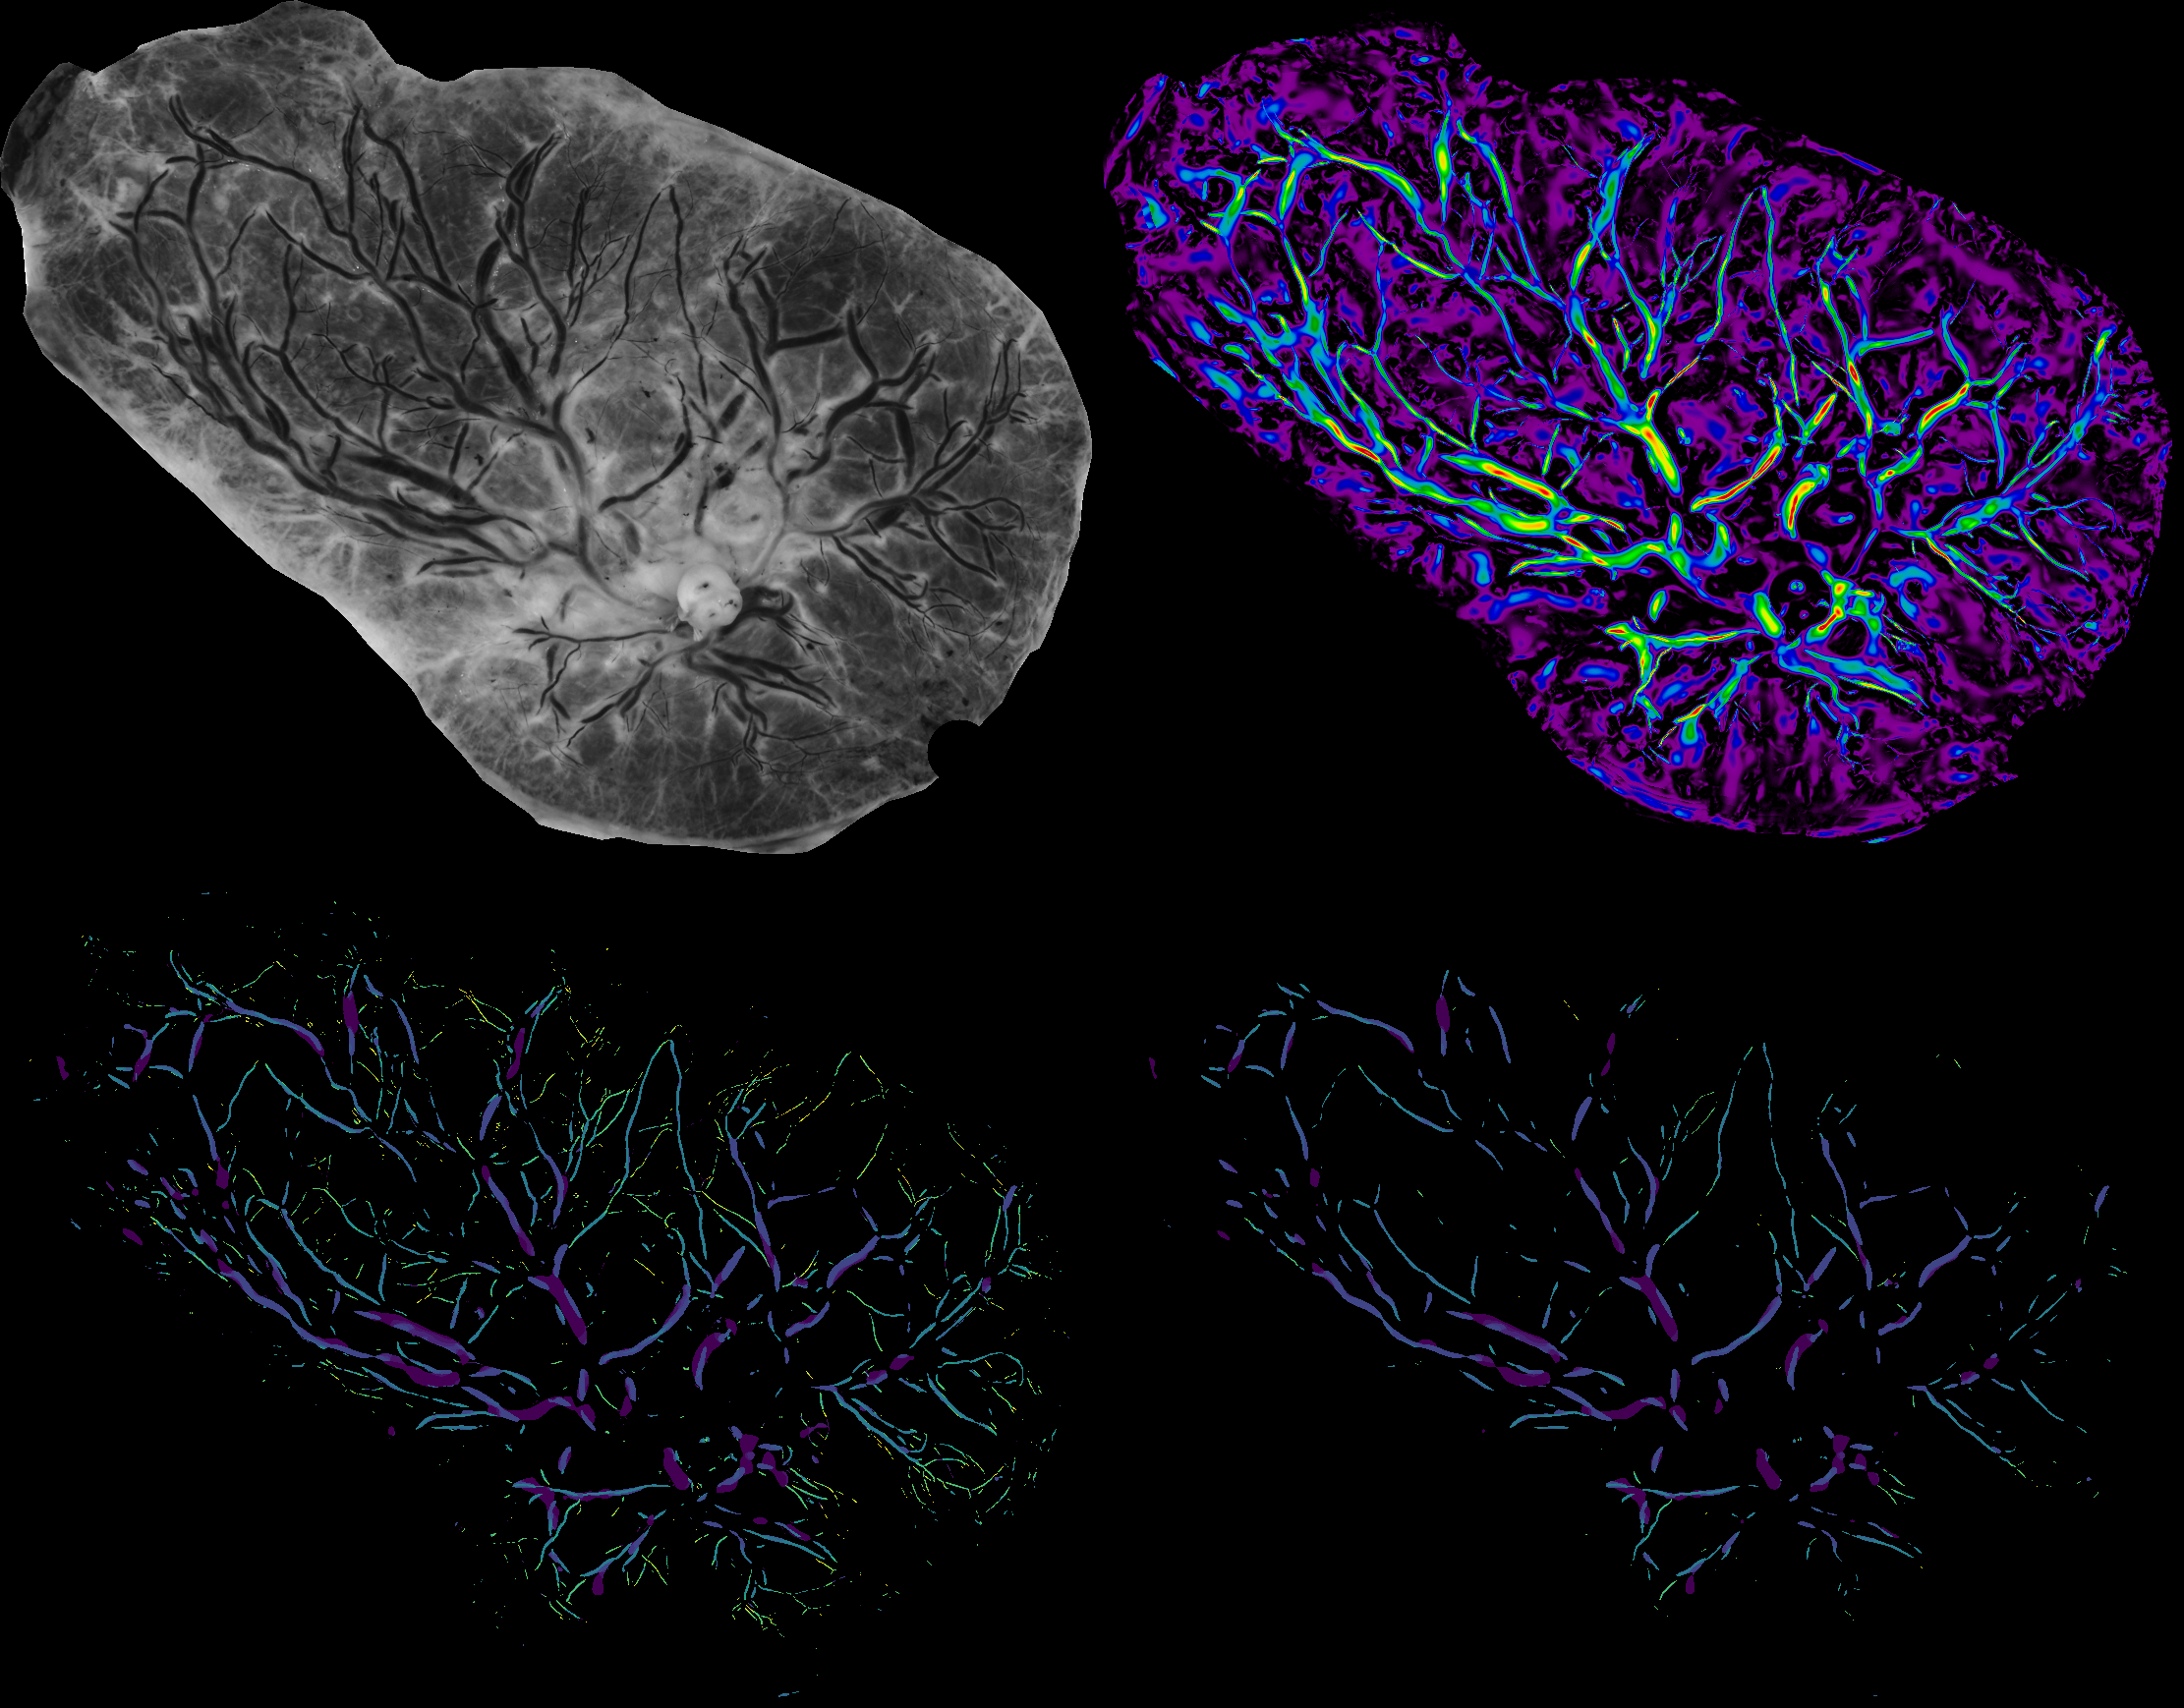
\includegraphics[width=\textwidth]{montage-T-BN0164923}
  \caption{Sample Multiscale Frangi output ($\beta=0.35$) with simple segmentation strategies (Example 1)}
  \label{fig:output-montage-example1}
\end{figure}

\begin{figure} \centering
  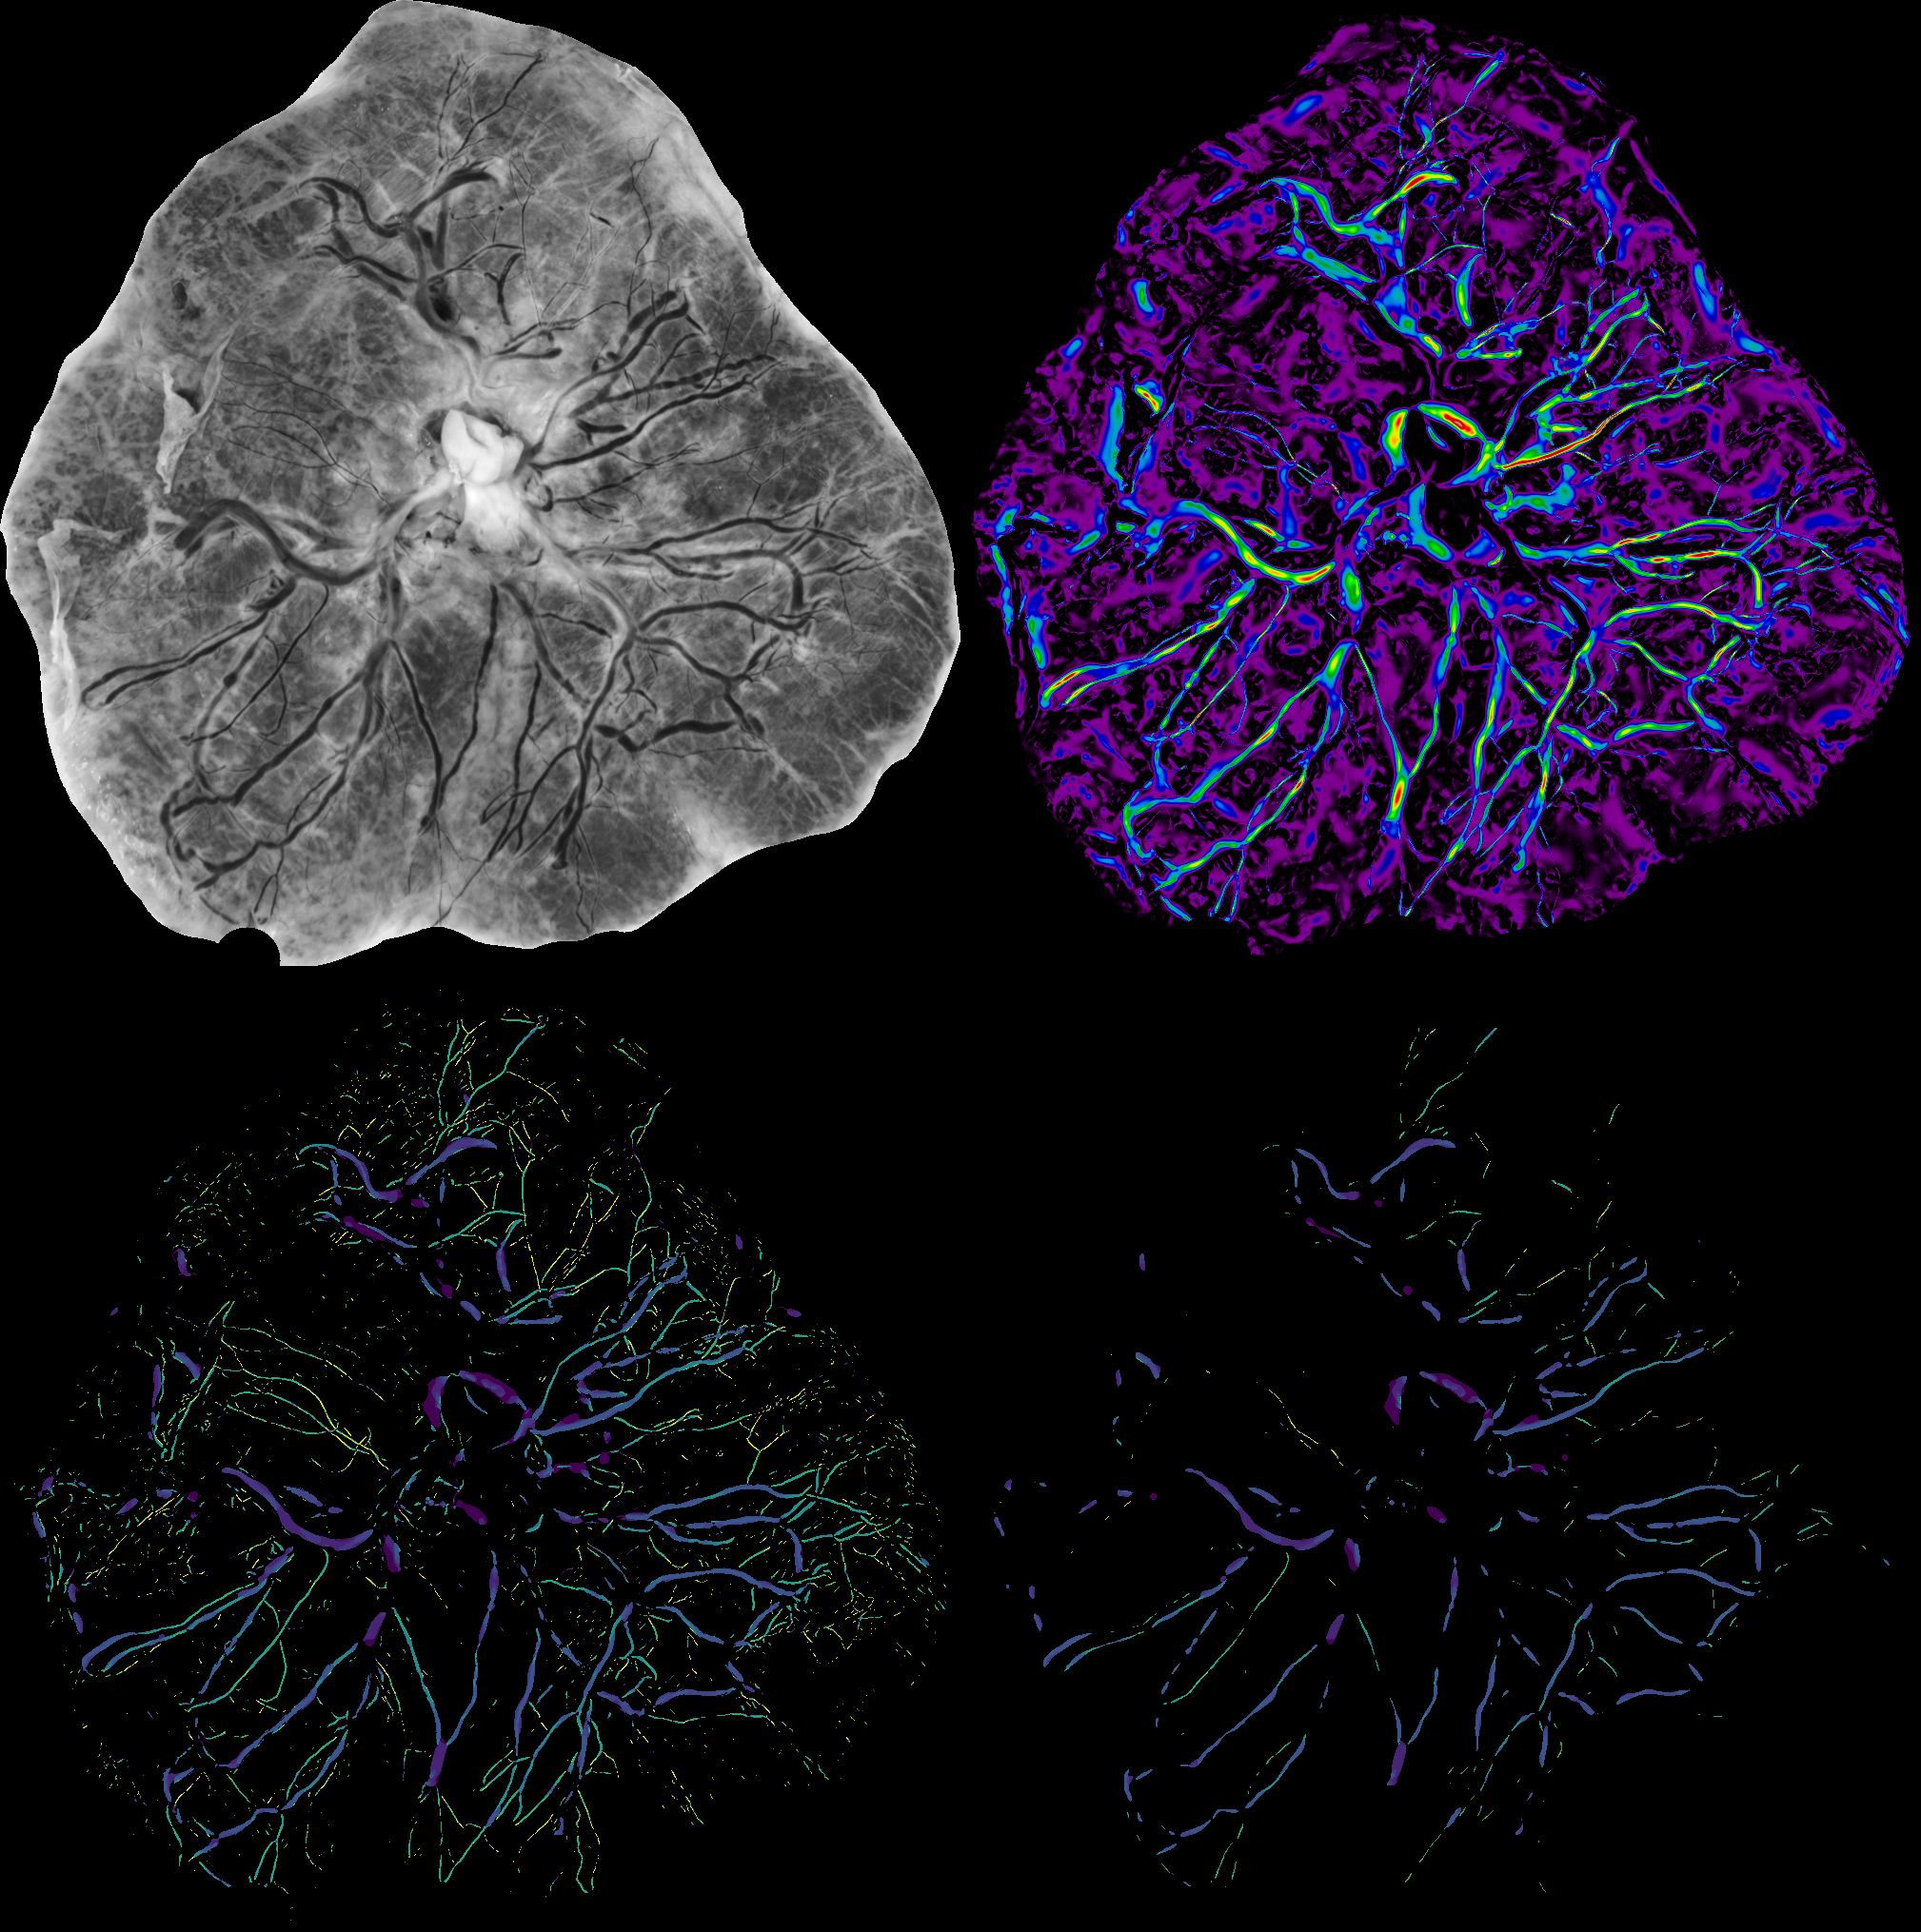
\includegraphics[width=\textwidth]{montage-T-BN0651415}
  \caption{Sample Multiscale Frangi output ($\beta=0.35$) with simple segmentation strategies (Example 2)}
  \label{fig:output-montage-example2}
\end{figure}


\begin{figure}
	\begin{minipage}[tp]{0.5\textwidth}
		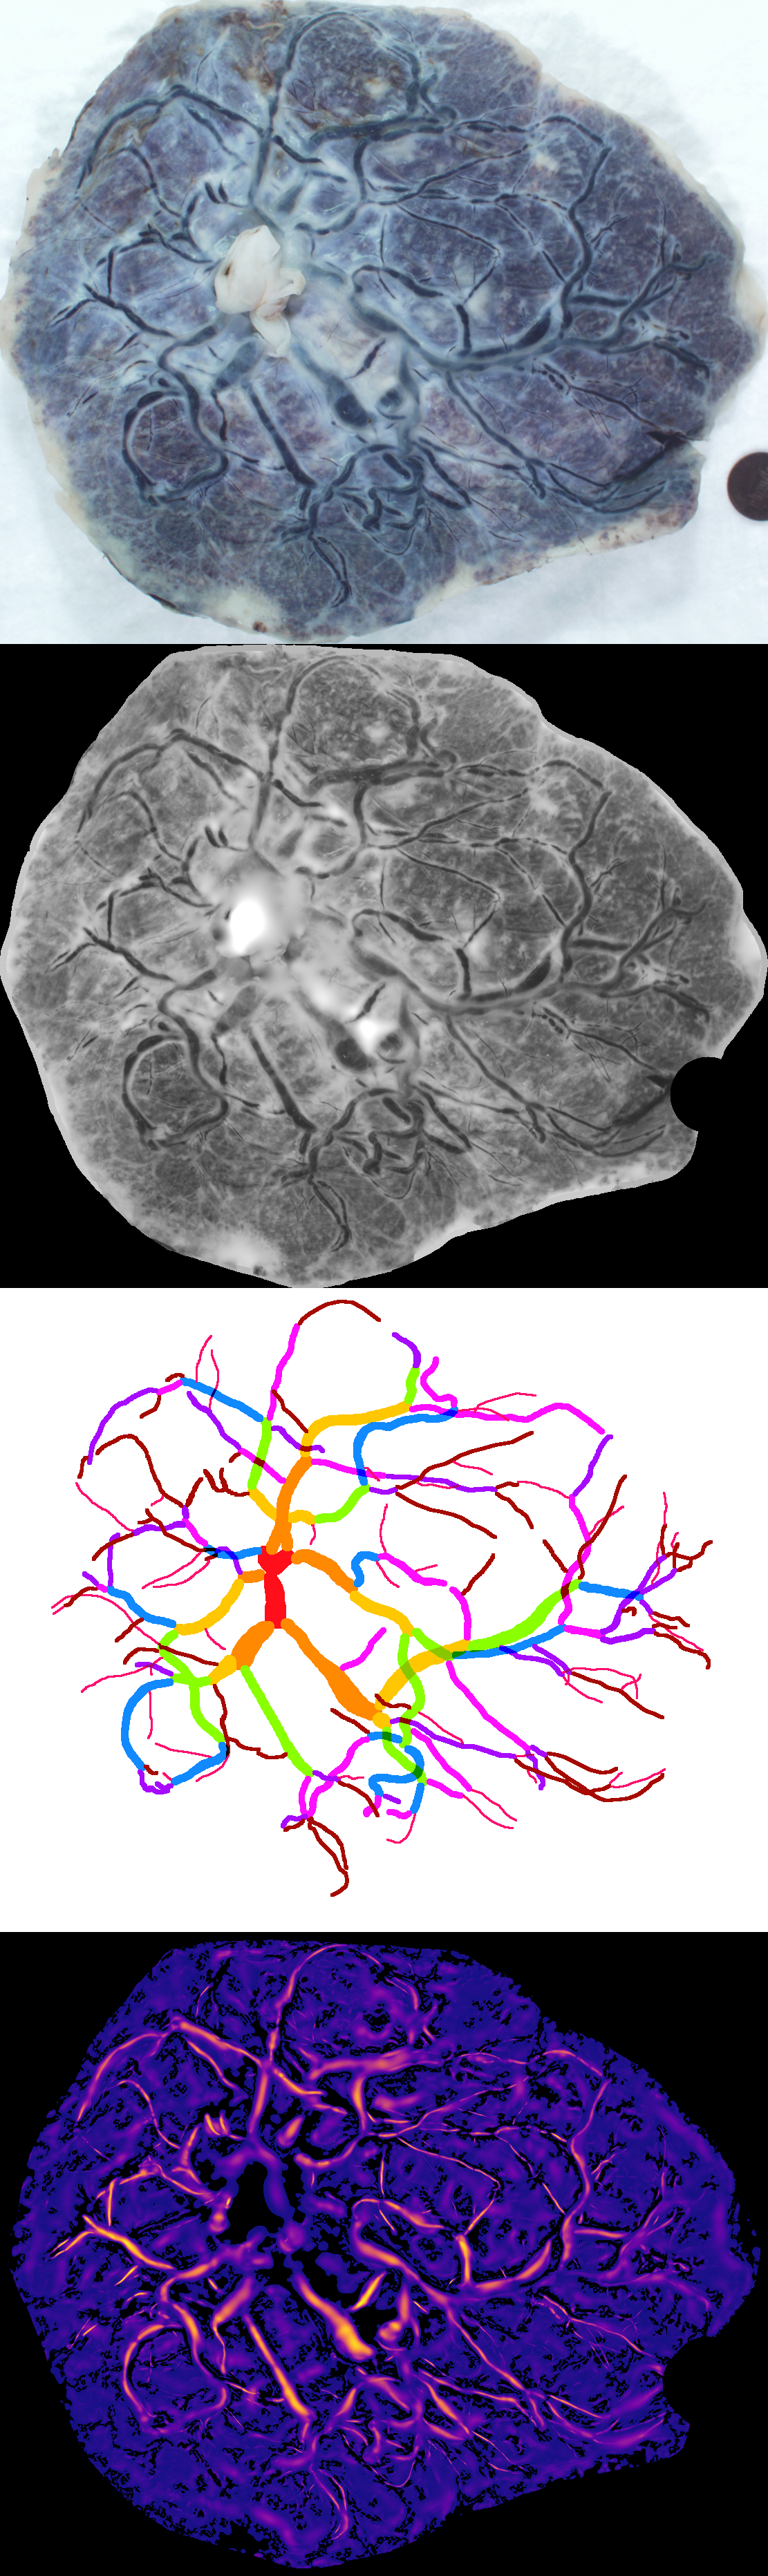
\includegraphics[height=0.95\textheight]{M1-T-BN2050224}
	\end{minipage}
	\quad
	\begin{minipage}[tp]{0.35\textwidth}
		\begin{tabular}{l|r|r|r}
			n  & $\sigma_n$  &  $\alpha_p$  &  $\max(V_\sigma)$ \\
			\hline
			0  &   0.3535 &  0.0547 &  0.986\\
			1  &   0.4243 &  0.0590 &  0.979\\
			2  &   0.5092 &  0.0654 &  0.970\\
			3  &   0.6110 &  0.0765 &  0.973\\
			4  &   0.7333 &  0.0892 &  0.988\\
			5  &   0.8801 &  0.0962 &  0.991\\
			6  &   1.0562 &  0.1082 &  0.991\\
			7  &   1.2676 &  0.1308 &  0.970\\
			8  &   1.5212 &  0.1669 &  0.973\\
			9  &   1.8256 &  0.2232 &  0.978\\
			10 &   2.1909 &  0.2925 &  0.984\\
			11 &   2.6294 &  0.3196 &  0.968\\
			12 &   3.1555 &  0.3269 &  0.994\\
			13 &   3.7869 &  0.3558 &  0.998\\
			14 &   4.5447 &  0.4058 &  0.999\\
			15 &   5.4542 &  0.3764 &  0.963\\
			16 &   6.5456 &  0.3184 &  0.950\\
			17 &   7.8553 &  0.3047 &  0.958\\
			18 &   9.4272 &  0.3287 &  0.916\\
			19 &  11.3137 &  0.3524 &  0.916\\
		\end{tabular} \\
	\end{minipage}
	\caption{Vesselness scores and percentile thresholds}
\end{figure}

\begin{figure}[p] \centering
	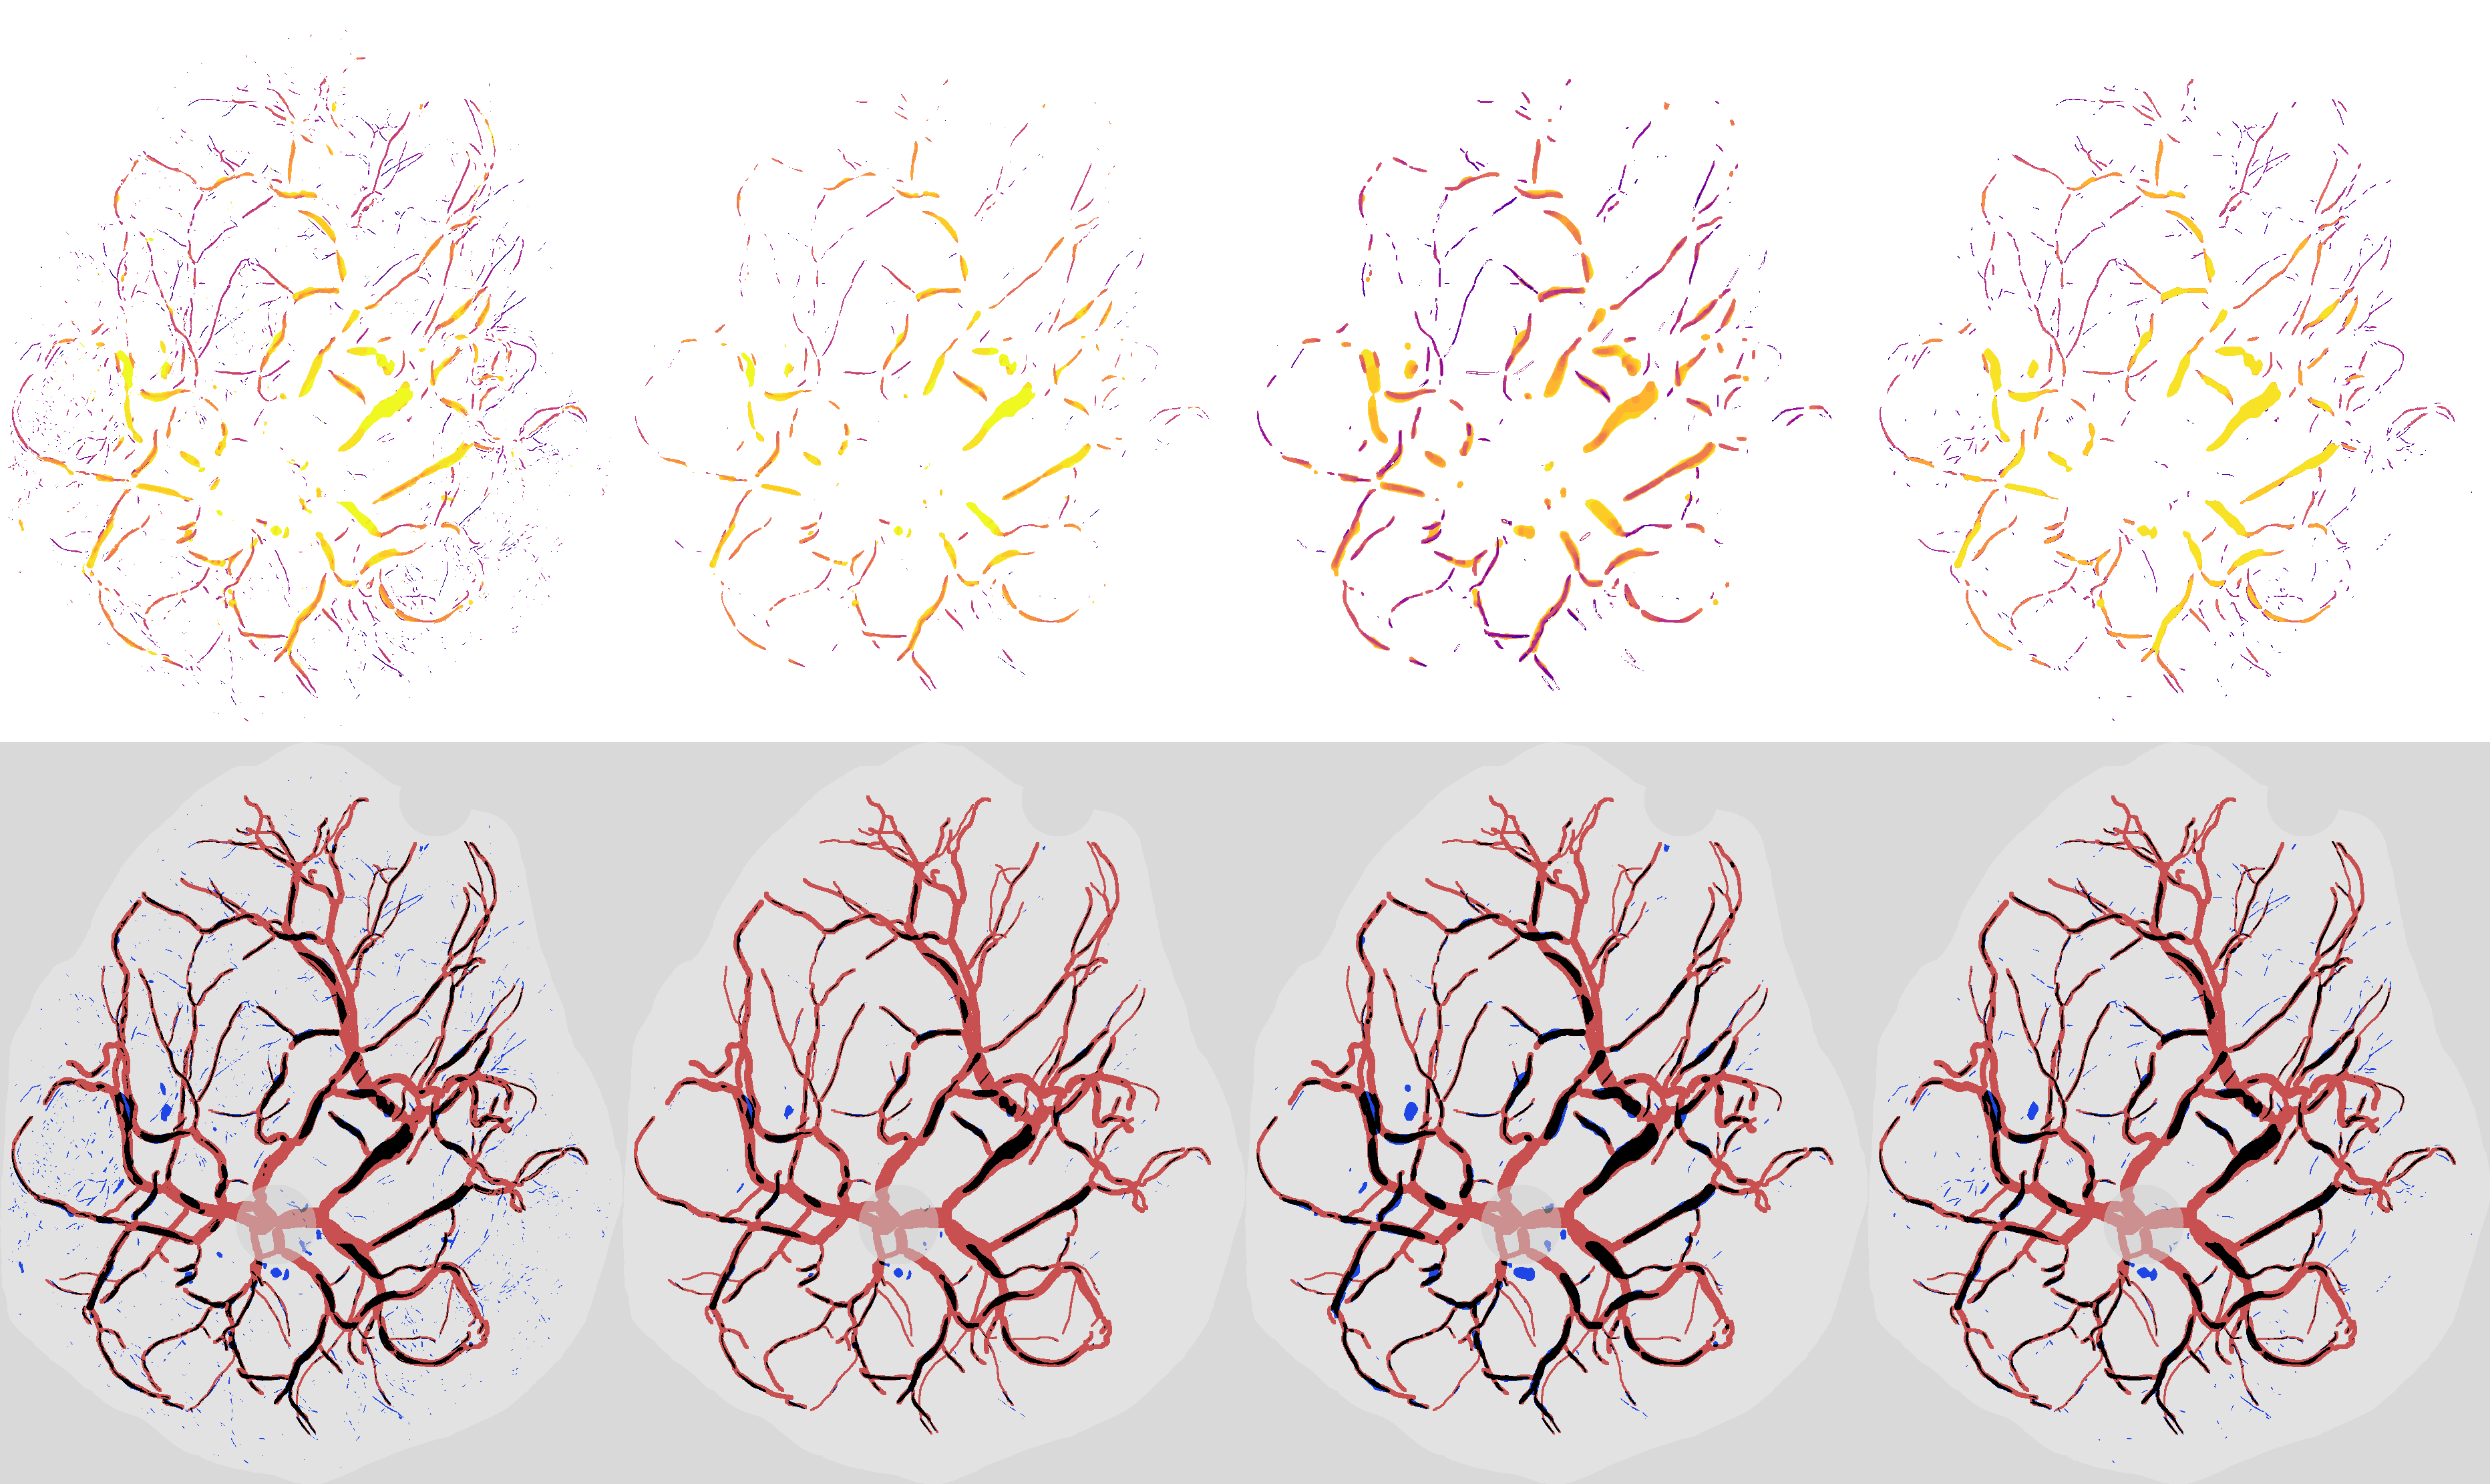
\includegraphics[width=\linewidth]{M2-T-BN2050224}
	\caption{Sample of Frangi-based Segmentation Methods (pt. 2)}
\end{figure}

\begin{table}[p]\centering
	\begin{tabular}{l|rrrr}
		{} &        PF &        FA &        RW &        PS \\
		\hline
		MCC           &  0.4872 &  0.4208 &  0.5249 &  0.4877 \\
		%\hline
		skel coverage &  0.5085 &  0.3245 &  0.4493 &  0.4650 \\
		%\hline
		precision     &  0.8044 &  0.9472 &  0.8858 &  0.8697 \\
	\end{tabular}
	\caption{Scores for merging techniques}
\end{table}

\section{Variations in the Data Set and Imperfections of the Ground Truth} \label{sec:NCS-dataset-issues}
\begin{sidewaysfigure}
	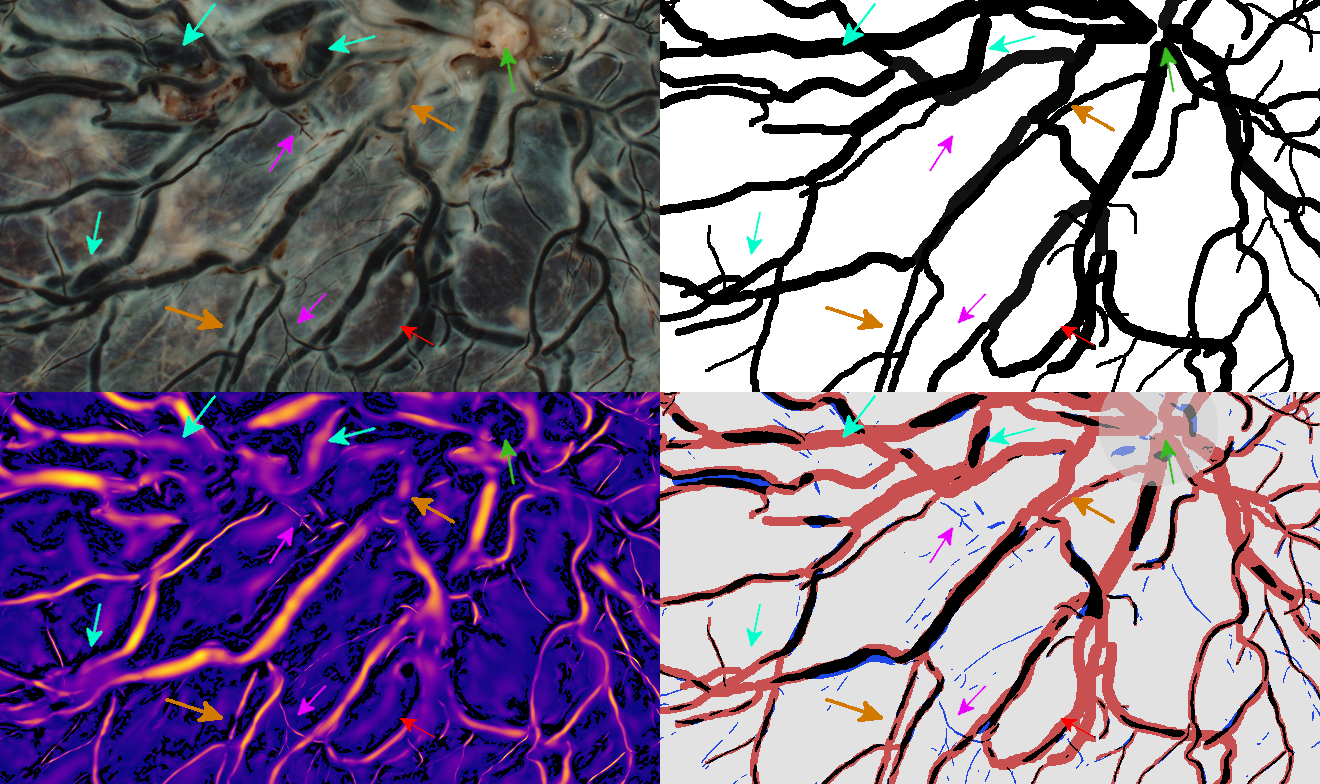
\includegraphics[width=\textwidth]{annotations-montage-2by2}
	\caption{Issues with the ground truth manifesting in Frangi vesselness scores}
	\label{fig:annotated-montage}
\end{sidewaysfigure}

We must qualify our binary classification. There are limitations to our ``the ground truth'' is not 100\% correct. In \cref{fig:annotated-montage} we demonstrate a few common issues with the samples. The four figures show (top left) the original colored raw sample, (top right) the ground truth tracing, (bottom left) \Vmax, and (bottom right) the confusion matrix after the "sieving strategy."  The green arrow points to the umbilical stump. You can see there is circular noise around this point, and in general perfusion around this point is very low--many of these vessels have been estimated by the tracer. The orange arrows represent points where perfusion is very low, like there is a clot in the vessel or something. The pink arrows point to vessels that were not traced, although they are clearly visible. The blue arrows point to where the shape of the vessel and the trace clearly do not agree. There any many more examples of these in the frame, and many more across all samples.

The red arrow points to an issue unrelated to the ground truth, but an issue that arise when selecting scales-- this is a point of dark curvature that represents noise at larger scales. As you can see from the \Vmax of this inset, there is a positive response in this dead space between vessels, and there is another one that appears in the bottom left between two close vessels of similar size. 

\begin{figure} \centering
  \subfloat{
  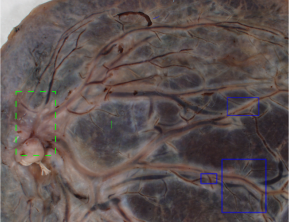
\includegraphics[width=0.5\textwidth]{T-BN0392644_inset}
}
\subfloat{
  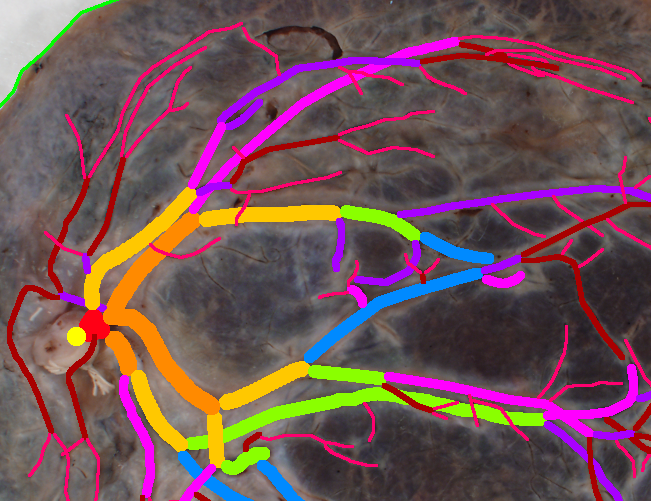
\includegraphics[width=0.5\textwidth]{T-BN0392644_inset_ctrace}
} \\
\subfloat{
  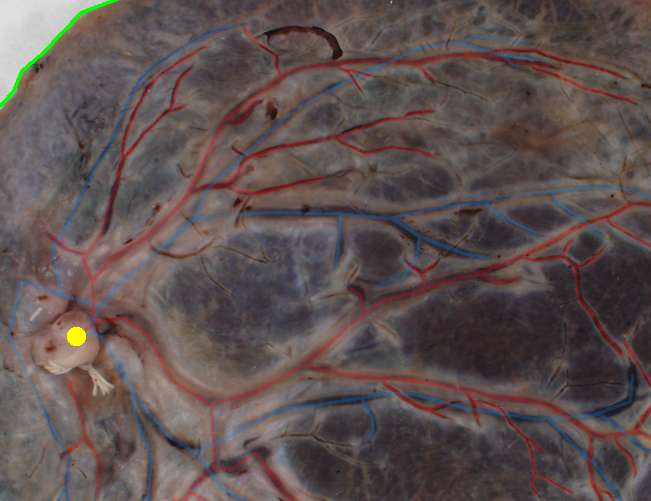
\includegraphics[width=0.5\textwidth]{T-BN0392644_inset_sketches}
}
\subfloat{
  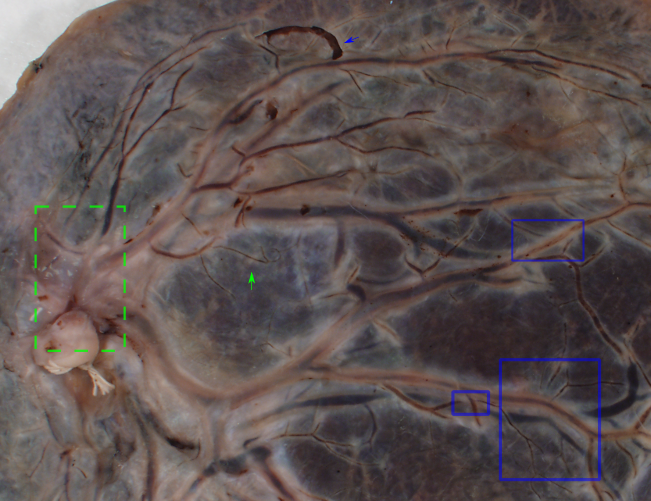
\includegraphics[width=0.5\textwidth]{T-BN0392644_inset_mark}
}
\caption{Issues with ground truth and sample quality}
\label{fig:groundtruth-samplequality}
\end{figure}

As seen in \cref{fig:groundtruth-samplequality}, there are several issues with the samples that will cause trouble in our efforts toward segmentation. Our represenative sample is BN0392644. The top left is the original (color) image, the top right is the full vessel width trace. The bottom left is a smaller skeletonization (sketch), where arteries are shown in red and veins are shown in blue. The bottom right figure contains some annotations. At the top, a blue arrow indicates a large curvilinear patch of dried blood that is not part of the vascular network. The green arrow in the middle indicates some vessels that are too small for the diameter binning and are thus not reported. We will see later that our Frangi result perfectly captures these, yet they will be reported as a false positive since they are not part of the tracing. However, there are other vessels of similar visual width in this same inset that are traced. In blue boxes (and in many other spots) the vessels cross each other. The border around these will prevent us from being able to extract the vessel directly. In the green dotted box, a major arterial and a major venous branch each connect to the umbilical cord insertion point. Whereas the arterial branch (on the right) can be seen, it will not be reported by the Frangi filter, since those points are not darker relative to the background. You can also see how much variation there is as you look along a blood vessel. There are some areas where the Frangi filter will have a very limited response. 



\begin{enumerate}
\item Collar is stupid and should really be considered like a error in marking the perimeter. Throw these away or edit. Maybe make a section called discarded samples that's stupid but yeah.
\item Vessels suck sometimes. In the portion above, 1602443, there's a random blood clot which gets identified at large $\sigma$. But also the small forked shaped thing which is obviously a vessel doesn't get defined.
\item Too much blood (not enough?? no idea) is left in the vessels. leading to the weird white border around some vessels. you could identify these along with black center and combine them somehow. no idea.Also, holy shit, some of the white vessel ``sleeves'' ARE identified in the tracing, and some aren't. Find an example of this and whine about it.
\item Umbillical cord insertion point is stupid and obscures a lot. The tracer guesses but there's no real guiding principle AFAIK..
\item Small vessels aren't accounted for at all. Not sure how to coincide measurement in terms of scale space anymore, but should figure out how to cut off those values before running MCC metric.
\end{enumerate}

An example of bad samples that performed comparatively poorly across all segmentation methods can be found in the \cref{bad_gallery}. You can see that there is a lot of "noise" on the sample itself, and in some cases the vessels are much larger than other samples and therefore weren't picked up.

\begin{figure}[p]
	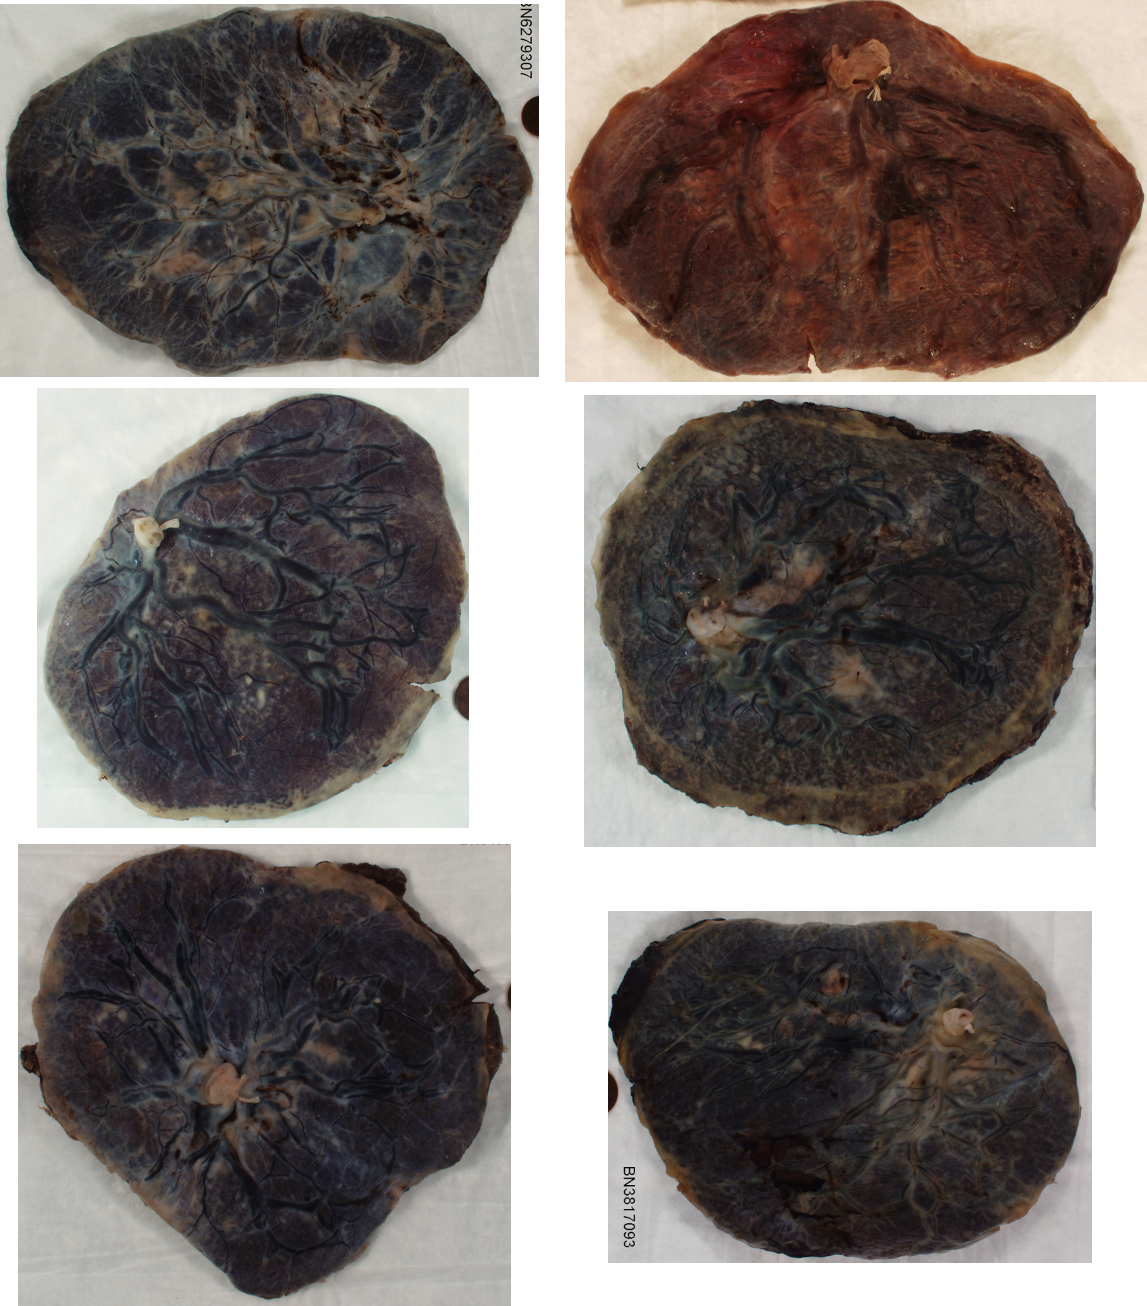
\includegraphics[width=\textwidth]{bad_gallery}
	\caption{Bad samples}
	\label{fig:bad-gallery}
\end{figure}

\section{Results}

In \cref{fig:compare_parameters}, we demonstrate the usefulness of scricter parameters for the Frangi filter. Since the Frangi vesselness measure is a "probability-like" score, we should be interested--without doing any actual segmentation yet--to what extent this score aligns with the ground truth in a cumulative sense. We should hope at least that larger values of We define the cumulative vesselness ratio by ``integrating'' the max vesselness score over pixels in the ground truth and over the entire image and considering the ratio:

\begin{defn} The cumulative vesselness ratio for a particular parametrization of the multiscale Frangi filter is given by
	\begin{equation}
	CVR\left(\Vmax\right) := \frac{\sum_{G\subset\img} \Vmax(x_0, y_0)}{\sum_{\img} \Vmax(x_0,y_0)}
	\end{equation}
	where the sums on top and bottom are being carried out for all pixels $(x_0,y_0)$ in the "ground truth" subset $G$ in the image $\img$
	and over the entire image $\img$ itself, respectively.
\end{defn}

\cref{fig:compare_parameters} shows $\Vmax$ for two well-behaved samples with reported $CVR$. We see in both cases that stricter parameters (smaller $\beta$ and larger $\gamma$) correspond to an increased $CVR$. Each of these sample was run over the same scales (logarithmically spaced from $2^{-1.5}$ to $2^{3.5}$ with $N=20$ and the color output of each $\Vmax$ is normalized between 0 and 1.

\begin{figure}[p]\centering
	\subfloat{
		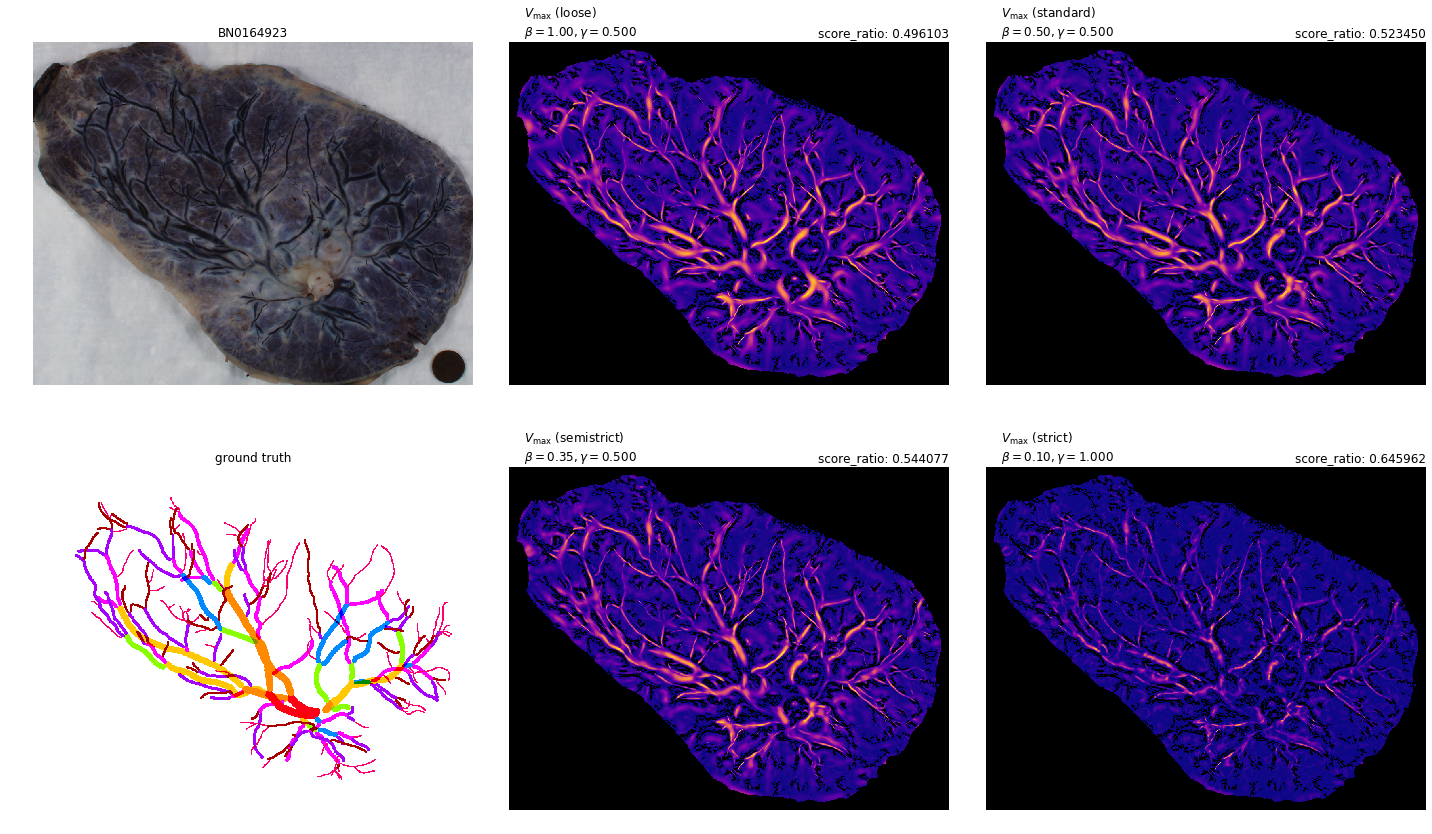
\includegraphics[width=\textwidth]{compare_parameters_BN0164923}
	}\\
	\subfloat{
		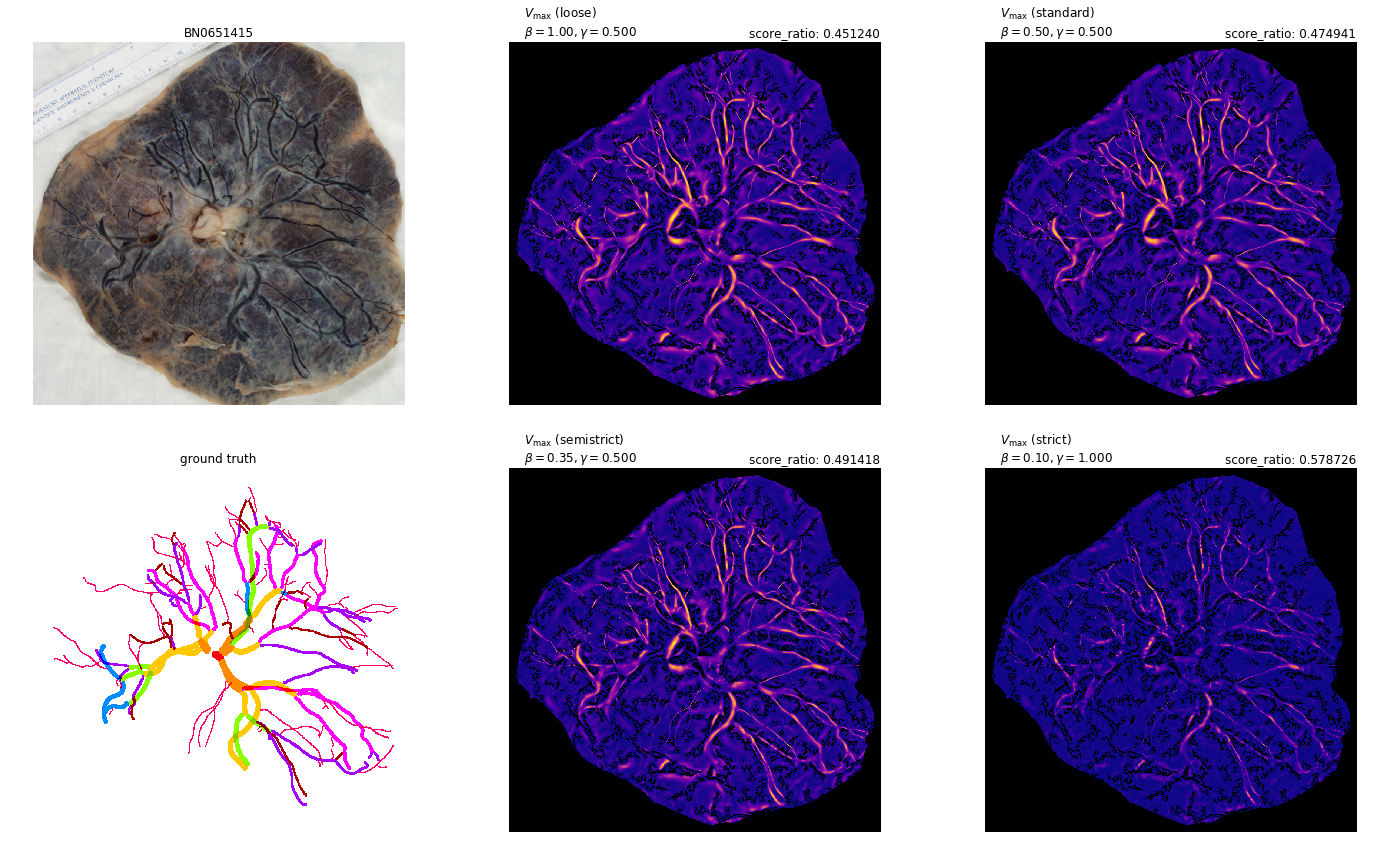
\includegraphics[width=\textwidth]{compare_parameters_BN0651415}
	}
	\caption{\Vmax  and $CVR$ for different parameter choices}
	\label{fig:compare_parameters}
\end{figure}

\begin{figure}[p]
  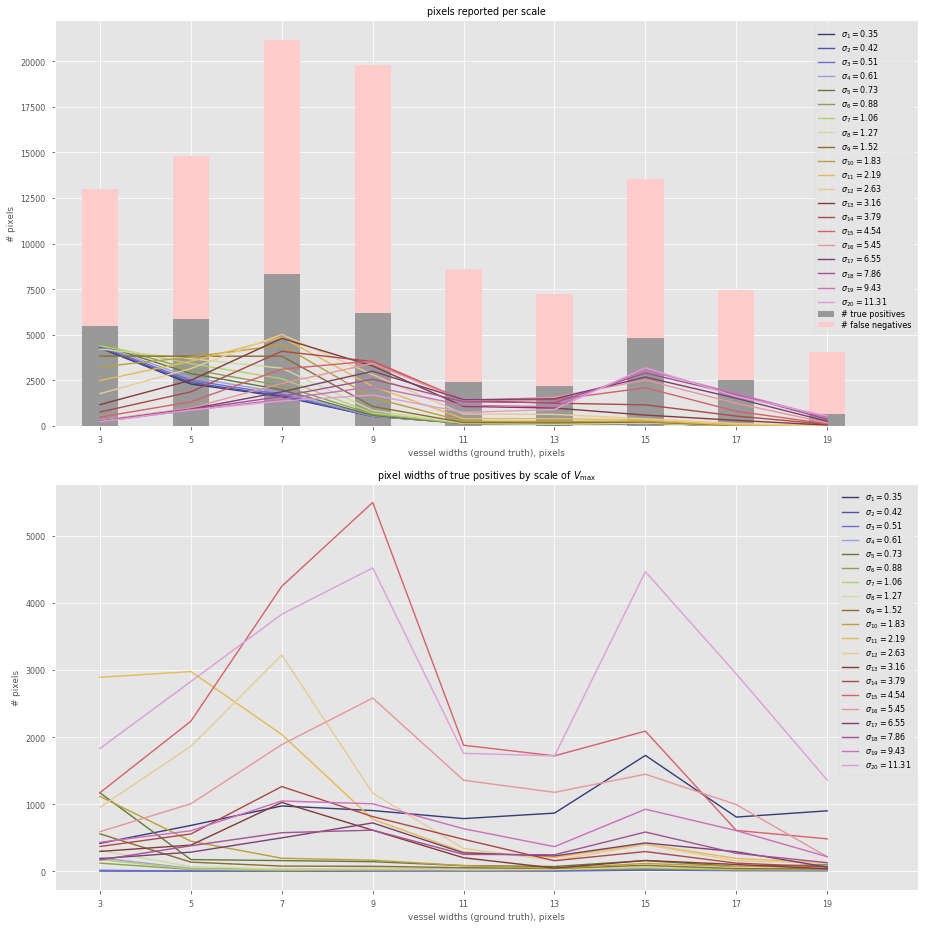
\includegraphics[width=\textwidth]{test-scale-width}
  \caption{Pixel Width of Ground Truth vs. Scale Length for True Positives}
\end{figure}

\begin{figure}[p]\centering
		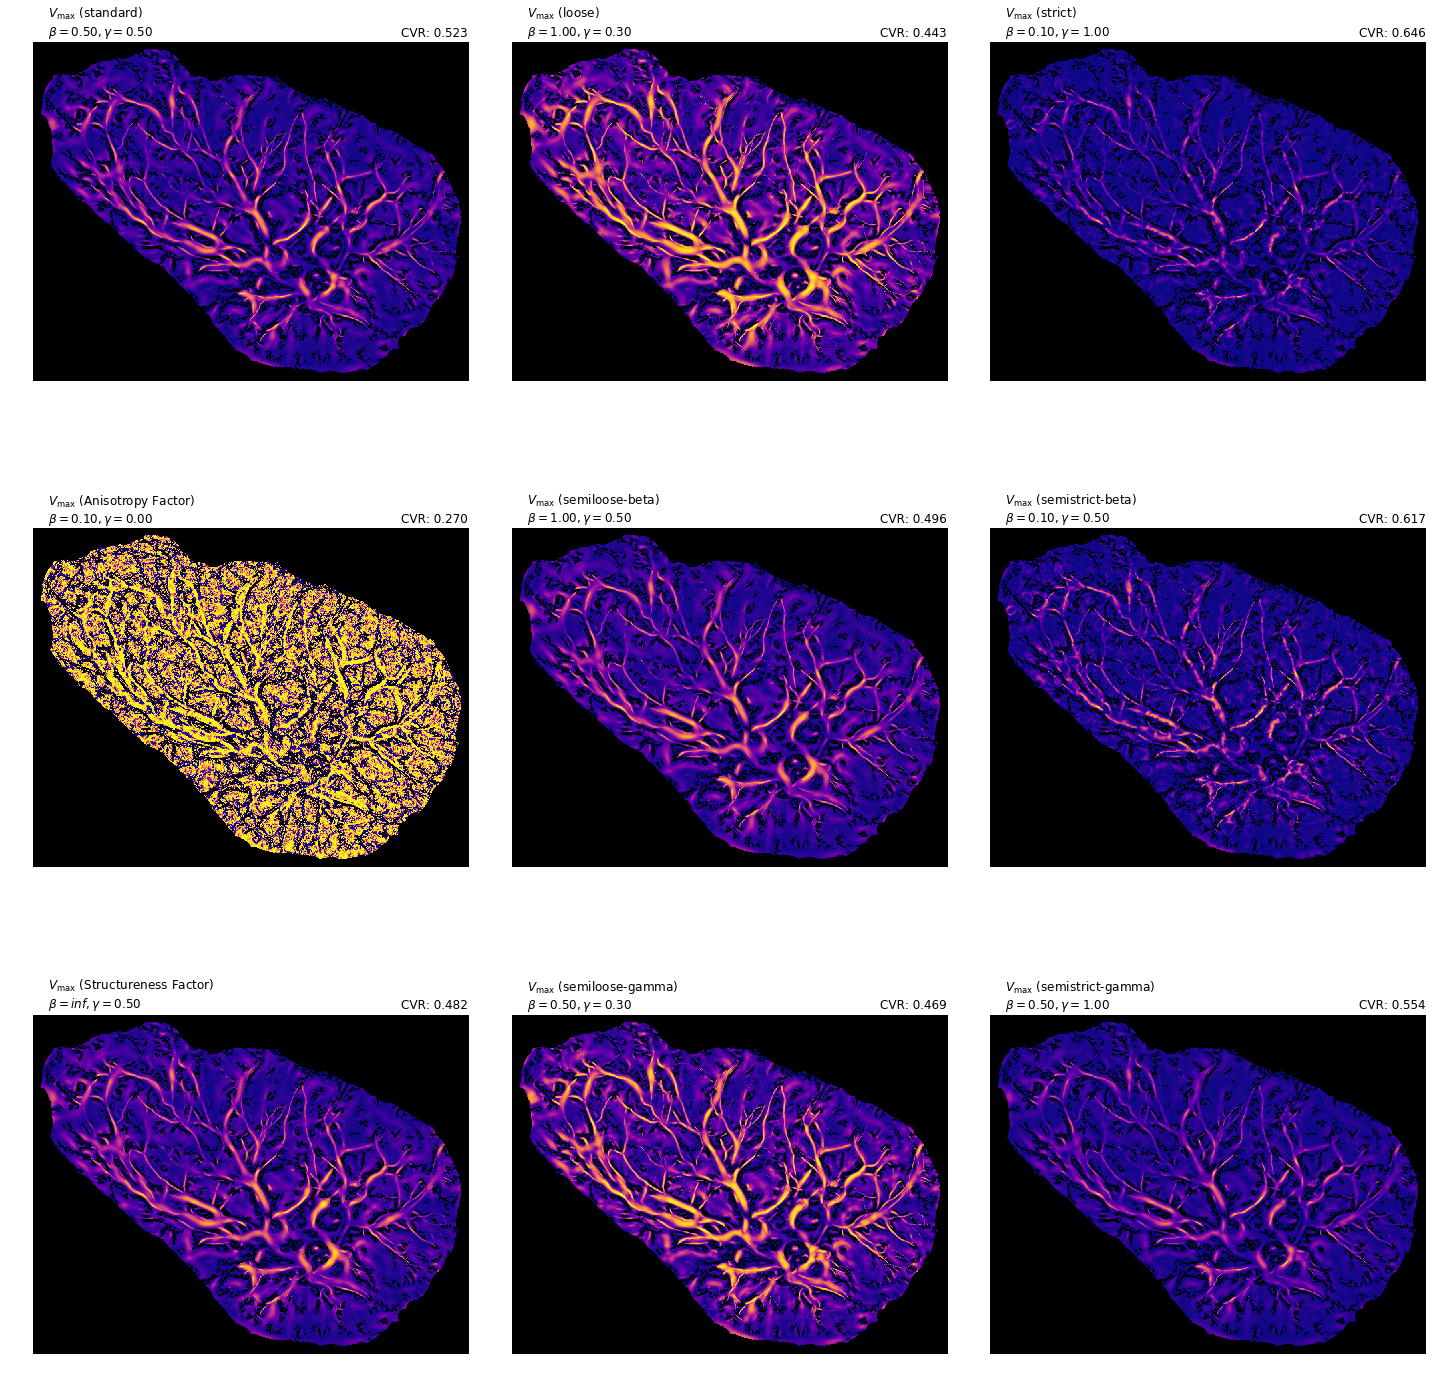
\includegraphics[width=\textwidth]{compare_parameters_3by3_example1}
	\caption{\Vmax  and $CVR$ for varying multiscale Frangi parametrizations (Example 1)}
	\label{fig:compare_parameters_3by3_example1}
\end{figure}

\begin{figure}[p]\centering
	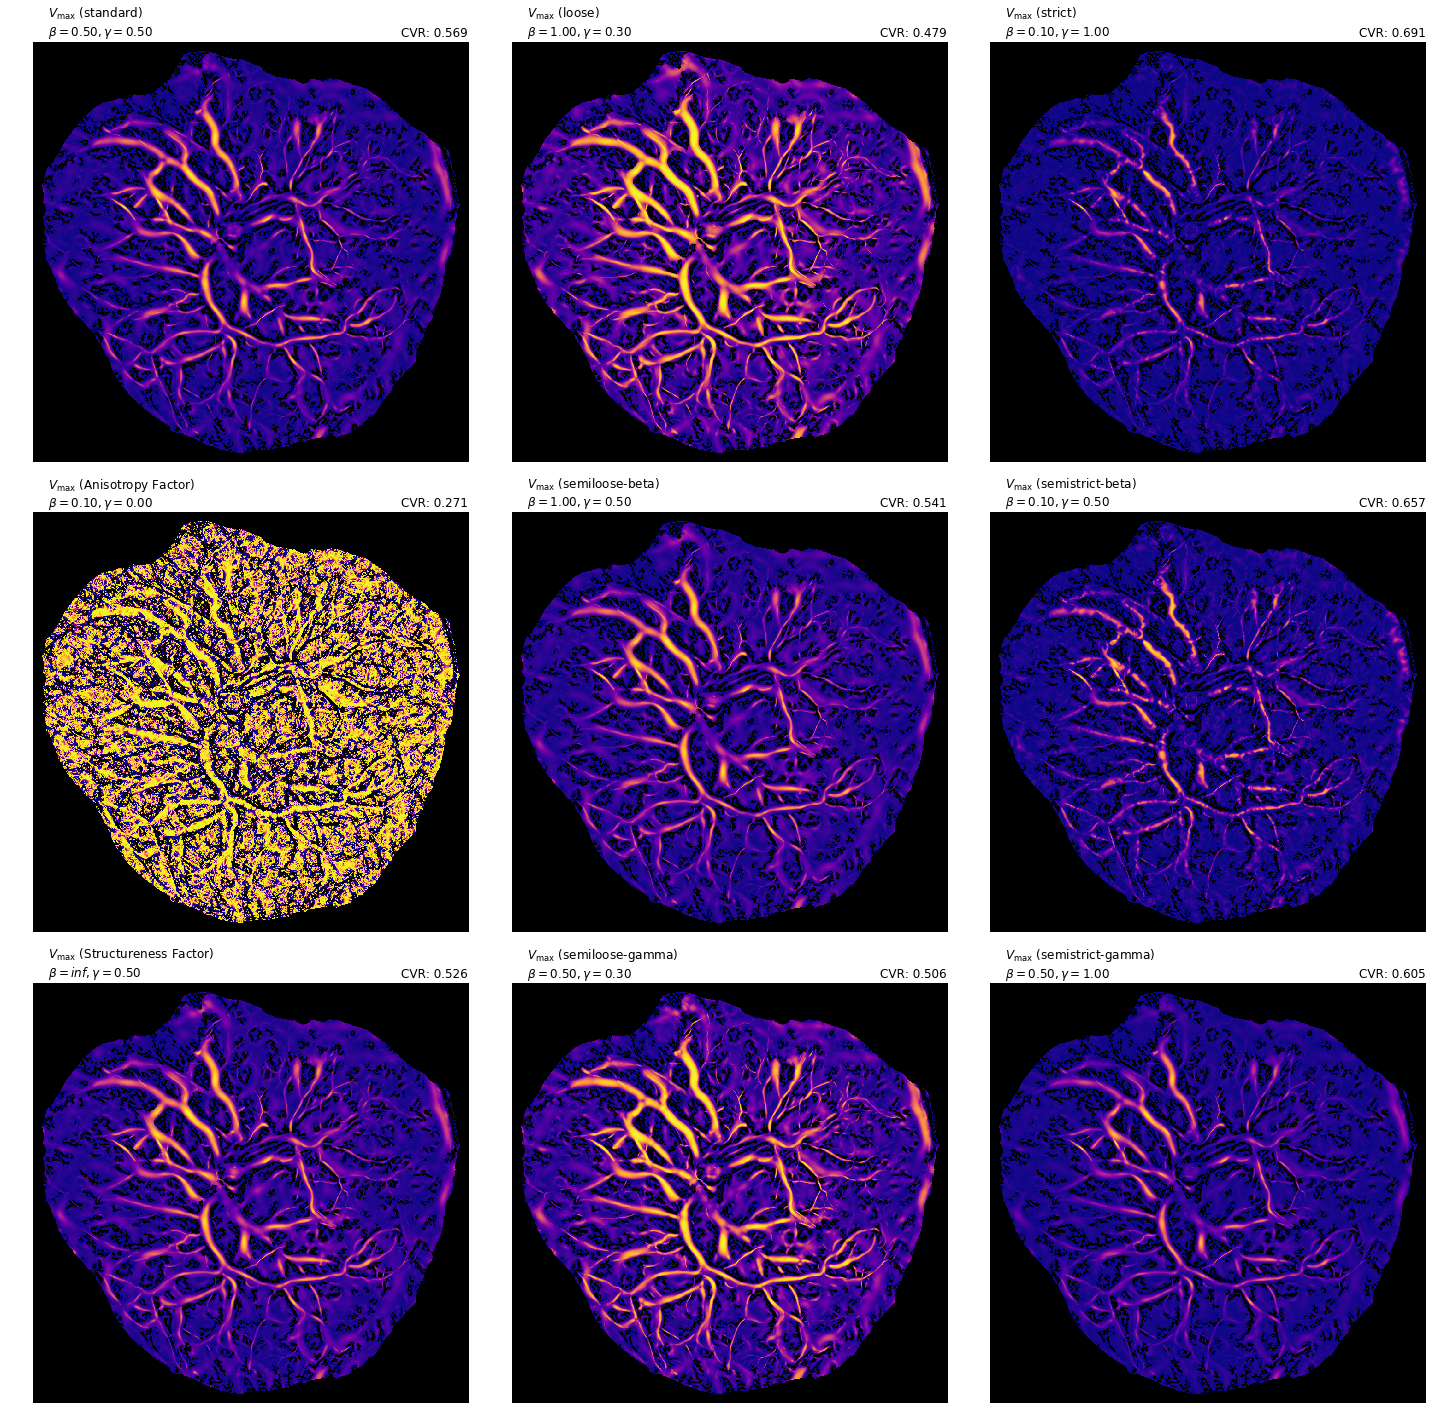
\includegraphics[width=\textwidth]{compare_parameters_3by3_example2}
	\caption{\Vmax  and $CVR$ for varying multiscale Frangi parametrizations (Example 2)}
	\label{fig:compare_parameters_3by3_example2}
\end{figure}

\begin{figure}\centering
	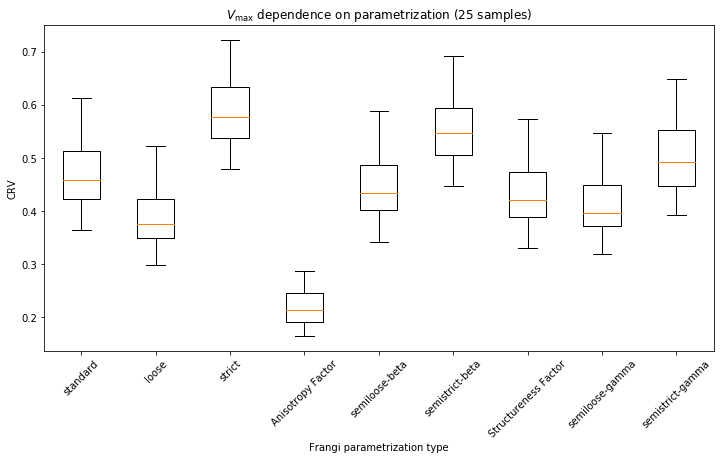
\includegraphics[width=\textwidth]{CRV_boxplot_quality0}
	\caption{$CVR$ scores of 25 samples under varying parametrizations}
  \label{fig:CVR-boxplot-quality0}
\end{figure}

In \cref{fig:CVR-boxplot-quality0} we show how the CVR is affected for 25 of the ``best'' samples, that is, those that generally fared better for segmentation techniques. This shows that the  results of \cref{fig:compare_parameters_3by3_example1} and \cref{fig:compare_parameters_3by3_example2} hold in general for all ``well-behaved'' samples in our image domain. 
\begin{figure}[p]\centering
  \subfloat{
  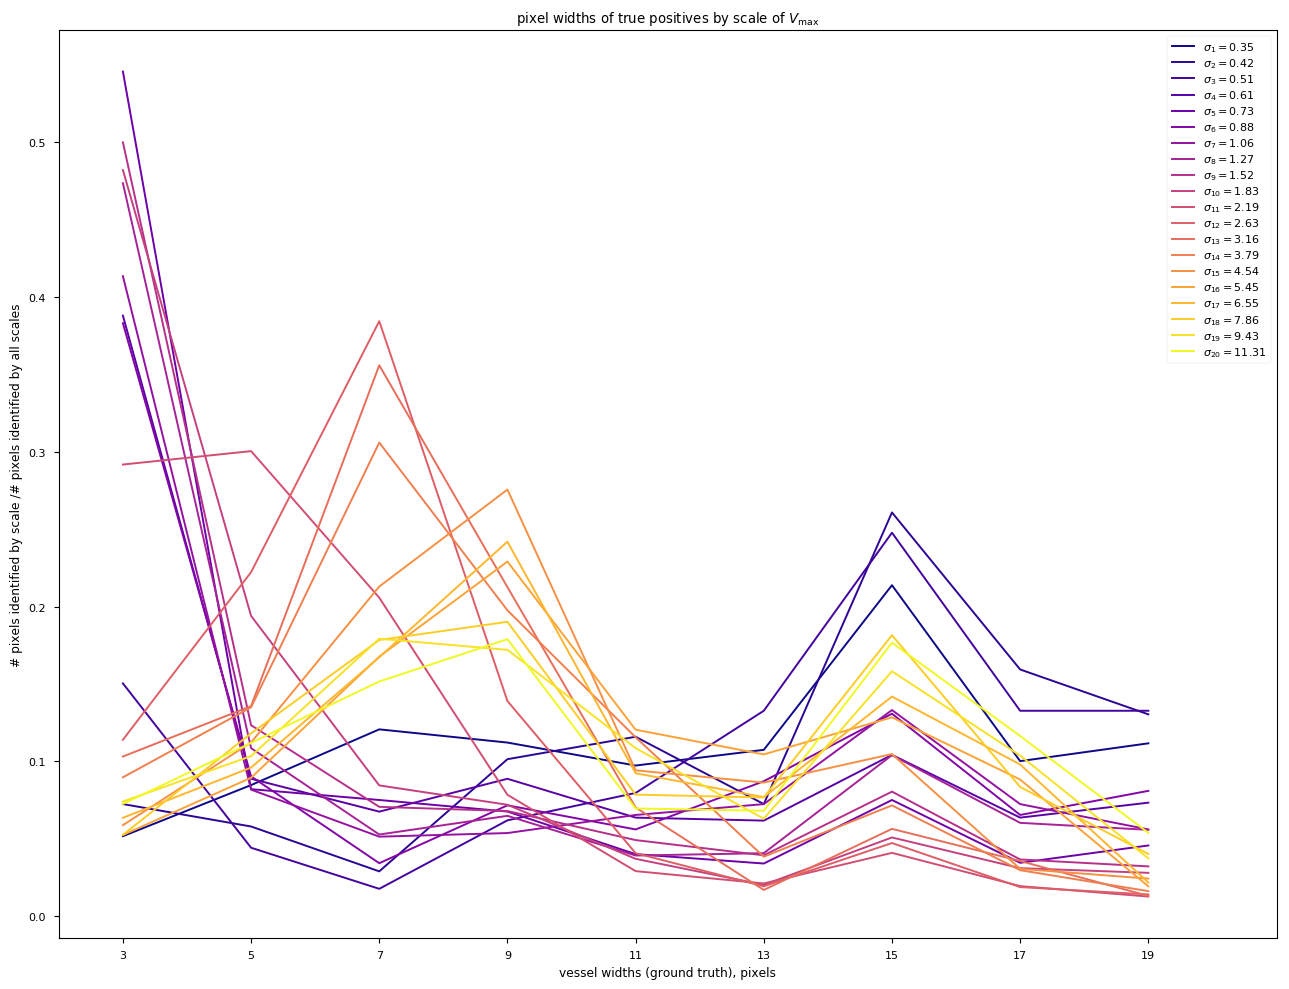
\includegraphics[width=0.85\textwidth]{Vmax_to_scale_normalized}
  }\\[-0.5cm]
  \subfloat{
  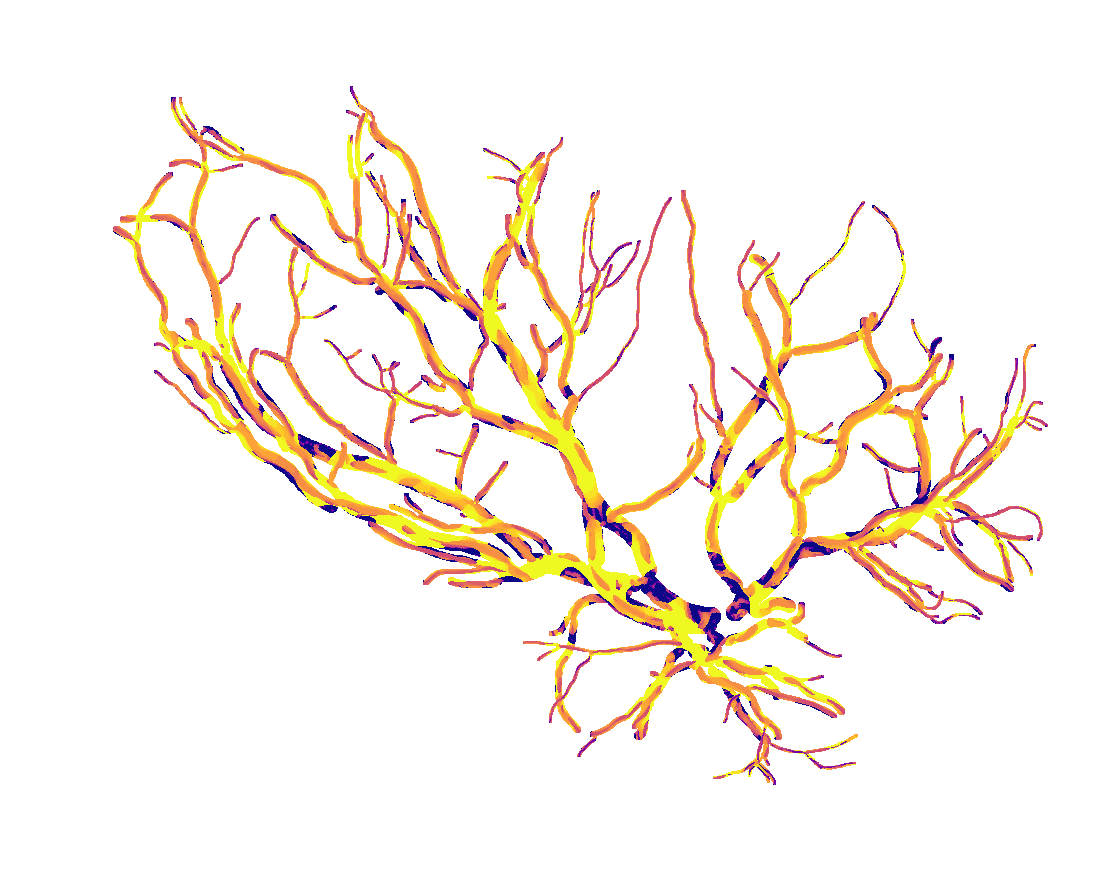
\includegraphics[width=0.85\textwidth]{frangi_argmax-trace}
  }
  \caption{Scale of maximum Frangi score for true positives and false negatives}
\end{figure}

\begin{figure}[p]\centering
  \subfloat{
    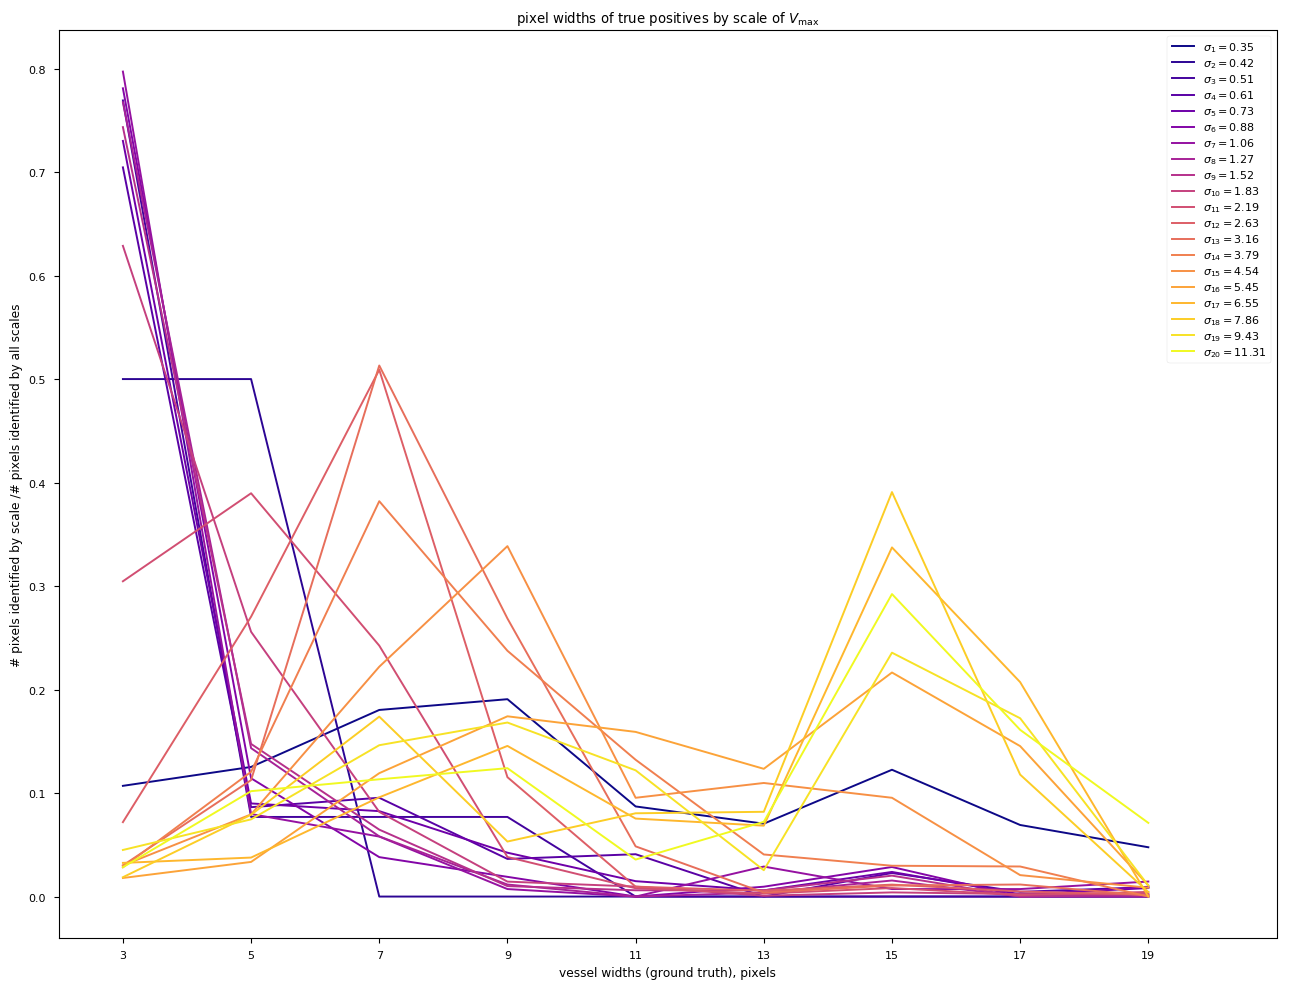
\includegraphics[width=0.85\textwidth]{Vmax_to_scale_normalized_with_approx}
  }\\[-0.5cm]
  \subfloat{
    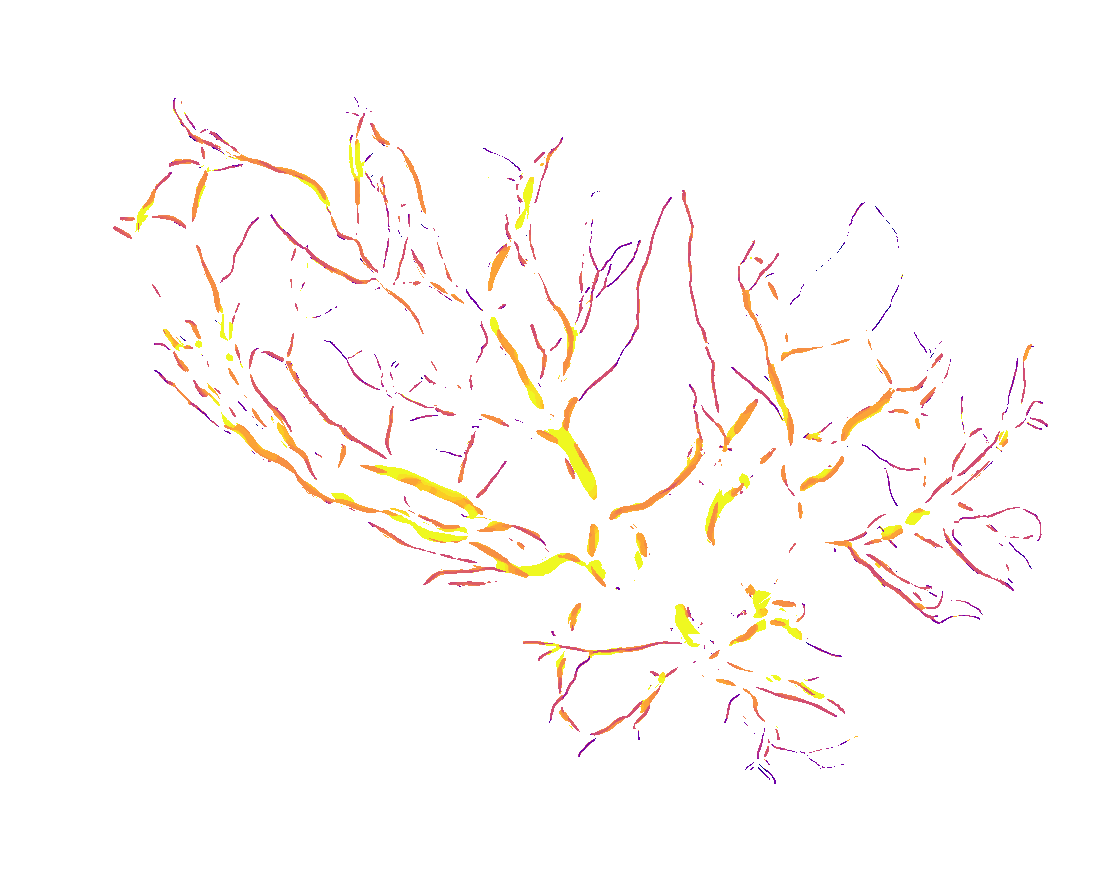
\includegraphics[width=0.85\textwidth]{frangi_argmax-trace-approx}
  }
  \caption{Scale of maximum Frangi score for true positives only (percentile filtering)}
\end{figure}

\chapter{Conclusion} \label{ch:conclusion}

We justified the use of differential geometry in 2D discrete image processing, and vastly improved upon the implementation of the Frangi filter. Our improved implementation allowed us to take more steps in our multiscale method and thus choose stricter parameters for Frangi scale. We used our multiscale Frangi vesselness measure to suggest several alternative approaches at merging the vesselness and compared their effectiveness as a precursor to segmentation and eventually network completion.

\section{Future research directions} \label{sec:future-research-directions}

\begin{itemize}
	\item Solve the Network Connection Problem (PICTURE OF GAPS)
	Try something like \cite{laptev2000automatic} or use of principal curvatures.
	\item Implement the automatic scale selection and normalization of derivates as mentioned in Lindeberg \cite{lindeberg1998feature} to relieve ourselves of
        our current dependency on manual selection of $\sigma_{\min}$ and  $\sigma_{\max}$.
	\item Look into gradient prefiltering more as well as varying $\gamma$ more, especially in areas where we suspect the network could be completed.
  \item Look into using signed frangi arguments.
	\item Use this as preprocessing for a Neural Network.
	(cite kara's work, katalinas work)
	\item Apply to more image domains (STARE, other placental domains).
	
\begin{figure}[p] \centering
	\subfloat{		\label{fig:signsweep-1p}\includegraphics[width=\linewidth]{{{signsweep_stitch_BN2315363_plate}}}
	} \\[-0.5cm]
	\subfloat{		\label{fig:signsweep-1i}\includegraphics[width=\linewidth]{{{signsweep_stitch_BN2315363_inset}}}
	} \\[-0.5cm]
	\subfloat{		
		\label{fig:signsweep-1c}\includegraphics[width=.75\linewidth]{{{signsweep_colorbar}}}
	} \\
	% should i use the real sample names? or obfuscate?
	\caption{Signed Frangi output (plate and inset) (Example 1)}
	\label{fig:signsweep-1}
\end{figure}

\begin{figure}[p] \centering
	\subfloat{		\label{fig:signsweep-2p}\includegraphics[width=\linewidth]{{{signsweep_stitch_BN5280796_plate}}}
	} \\[-0.5cm]
	\subfloat{		\label{fig:signsweep-2i}\includegraphics[width=\linewidth]{{{signsweep_stitch_BN5280796_inset}}}
	} \\[-0.5cm]
	\subfloat{		
		\label{fig:signsweep-2c}\includegraphics[width=.75\linewidth]{{{signsweep_colorbar}}}
	} \\
	% should i use the real sample names? or obfuscate?
	\caption{Signed Frangi output (plate and inset) (Example 1)}
	\label{fig:signsweep-2}
\end{figure}

\end{itemize}




\HalfPage{Appendices}
%% Renews chapter command so type appendix files in the same way

\myappendix{Code Listings}
%% Here is the appendix (not needed.)

The following python scripts and modules were developed with the following packages:

\begin{itemize}
\item \texttt{python 3.6}
\item \texttt{numpy}, version 1.12.0
\item \texttt{scipy}, version 0.19.0
\item \texttt{scikit-image}, version 0.13.0 
\item \texttt{matplotlib}, version 2.02
\end{itemize}
%
Earlier versions of these packages may be compatible but are not guaranteed to be so. 
The scripts listed in this appendix are also hosted at
\texttt{github.com/wukm/pycake}.
%\lstinputlisting[language=python]{abbreviate_NCS_names.py}
\lstinputlisting[language=python]{add_margins.py}
%\lstinputlisting[language=python]{alpha_sweep_demo.py}
%\lstinputlisting[language=python]{basic.py}
%\lstinputlisting[language=python]{boundarycalcs.py}
\lstinputlisting[language=python]{cut_demo.py}
%\lstinputlisting[language=python]{cutfixer.py}
\lstinputlisting[language=python]{diffgeo.py}
%\lstinputlisting[language=python]{dilate_by_distance.py}
\lstinputlisting[language=python]{extract_NCS_pcsvn.py}
%\lstinputlisting[language=python]{farm_samples.py}
%\lstinputlisting[language=python]{finalfigstoshowmash.py}
\lstinputlisting[language=python]{frangi_graphing.py}
%\lstinputlisting[language=python]{frangi-plottesting.py}
\lstinputlisting[language=python]{frangi.py}
\lstinputlisting[language=python]{gradient_filter_demo.py}
%\lstinputlisting[language=python]{gradient_filter_mash.py}
\lstinputlisting[language=python]{hfft_accuracy.py}
\lstinputlisting[language=python]{hfft_demo.py}
\lstinputlisting[language=python]{hfft.py}
%\lstinputlisting[language=python]{make_metadata.py}
\lstinputlisting[language=python]{make_output_montage.py}
\lstinputlisting[language=python]{merging.py}
%\lstinputlisting[language=python]{output-montages}
\lstinputlisting[language=python]{pcsvn.py}
\lstinputlisting[language=python]{pd_demo_uniscale.py}
\lstinputlisting[language=python]{placenta.py}
\lstinputlisting[language=python]{plate_morphology.py}
\lstinputlisting[language=python]{postprocessing.py}
\lstinputlisting[language=python]{preprocessing.py}
\lstinputlisting[language=python]{process_NCS_xcfs.py}
\lstinputlisting[language=python]{scaledecay.py}
%\lstinputlisting[language=python]{scale_sweep_demo_old.py}
\lstinputlisting[language=python]{scale_sweep_demo.py}
%\lstinputlisting[language=python]{scaletowidthplots.py}
\lstinputlisting[language=python]{scoring.py}
\lstinputlisting[language=python]{signed_sweep_demo.py}
%\lstinputlisting[language=python]{vessel_filters.py}
%\lstinputlisting[language=python]{visualize_sobel.py}

%Here is the list of cited works.
\HalfPage{Bibliography}


%% use Zotero to create bibliography
%% then export in BibTeX format into file thesis_bib.bib
%\bibliographystyle{prsty} % this was the default
\bibliographystyle{plain-annote} %annotated version
\bibliography{thesis_bib}
%\nocite{*}

\end{document}
